\documentclass[8pt]{beamer}

\usepackage[meeting={CTA Consortium Meeting},
            date={La Palma, 2017-11-07},
            title={first full sensitivity with the pipepline prototype},
            shorttitle={ctapipe}]{beamersetup}

\usepackage{wasysym}

\begin{document}

    \begin{frame}
        \titlepage
    \end{frame}


    \begin{frame}{Array Layout}
        \begin{columns}
            \column{.6\textwidth}
                \setlength{\figureheight}{\textwidth}
                \setlength{\figurewidth}{\textwidth}
                % This file was created by matplotlib2tikz v0.6.13.
\begin{tikzpicture}

\definecolor{color0}{rgb}{0.12156862745098,0.466666666666667,0.705882352941177}
\definecolor{color1}{rgb}{1,0.498039215686275,0.0549019607843137}
\definecolor{color2}{rgb}{0.172549019607843,0.627450980392157,0.172549019607843}

\begin{axis}[
title={HB9 L+N+D},
xlabel={$x / \mathrm{m}$},
ylabel={$y / \mathrm{m}$},
xtick={-1200,-800,...,1200},
ytick={-1200,-800,...,1200},
xmin=-1500, xmax=1500,
ymin=-1500, ymax=1500,
width=\figurewidth,
height=\figureheight,
tick align=outside,
tick pos=left,
x grid style={lightgray!92.026143790849673!black},
y grid style={lightgray!92.026143790849673!black},
legend style={draw=white!80.0!black,opacity=.75},
legend entries={{LST:LSTCam},{MST:NectarCam},{SST-1M:DigiCam}},
legend cell align={left}
]
\addplot [only marks, draw=color0, fill=color0, opacity=0.5, colormap/viridis, visualization depends on={\thisrow{sizedata} \as\perpointmarksize}, scatter/@pre marker code/.append style={/tikz/mark size=\perpointmarksize}]
table{%
x                      y                      sizedata
-2.000000000000000e+01 +6.500000000000000e+01 +5.315394051150731e+00
-2.000000000000000e+01 -6.500000000000000e+01 +5.315394051150731e+00
+8.000000000000000e+01 +0.000000000000000e+00 +5.315394051150731e+00
-1.200000000000000e+02 +0.000000000000000e+00 +5.315394051150731e+00
};
\addplot [only marks, draw=color1, fill=color1, opacity=0.5, colormap/viridis, visualization depends on={\thisrow{sizedata} \as\perpointmarksize}, scatter/@pre marker code/.append style={/tikz/mark size=\perpointmarksize}]
table{%
x                      y                      sizedata
+0.000000000000000e+00 +0.000000000000000e+00 +3.826166692590998e+00
+0.000000000000000e+00 +1.511999969482422e+02 +3.826166692590998e+00
+0.000000000000000e+00 -1.511999969482422e+02 +3.826166692590998e+00
+1.466559906005859e+02 +7.559999847412109e+01 +3.826166692590998e+00
+1.466559906005859e+02 -7.559999847412109e+01 +3.826166692590998e+00
-1.466559906005859e+02 +8.559999847412109e+01 +3.826166692590998e+00
-1.466559906005859e+02 -8.559999847412109e+01 +3.826166692590998e+00
+1.542050018310547e+02 +2.384739990234375e+02 +3.826166692590998e+00
+1.542050018310547e+02 -2.384739990234375e+02 +3.826166692590998e+00
+3.084100036621094e+02 +0.000000000000000e+00 +3.826166692590998e+00
-1.542050018310547e+02 +2.384739990234375e+02 +3.826166692590998e+00
-1.542050018310547e+02 -2.384739990234375e+02 +3.826166692590998e+00
-3.084100036621094e+02 +0.000000000000000e+00 +3.826166692590998e+00
+0.000000000000000e+00 +3.252420043945312e+02 +3.826166692590998e+00
+0.000000000000000e+00 -3.252420043945312e+02 +3.826166692590998e+00
+3.154680175781250e+02 +1.626210021972656e+02 +3.826166692590998e+00
+3.154680175781250e+02 -1.626210021972656e+02 +3.826166692590998e+00
-3.154680175781250e+02 +1.626210021972656e+02 +3.826166692590998e+00
-3.154680175781250e+02 -1.626210021972656e+02 +3.826166692590998e+00
+2.910849914550781e+02 +4.501549987792969e+02 +3.826166692590998e+00
+2.910849914550781e+02 -4.501549987792969e+02 +3.826166692590998e+00
+5.821699829101562e+02 +0.000000000000000e+00 +3.826166692590998e+00
-2.910849914550781e+02 +4.501549987792969e+02 +3.826166692590998e+00
-2.910849914550781e+02 -4.501549987792969e+02 +3.826166692590998e+00
-5.821699829101562e+02 +0.000000000000000e+00 +3.826166692590998e+00
};
\addplot [only marks, draw=color2, fill=color2, opacity=0.5, colormap/viridis, visualization depends on={\thisrow{sizedata} \as\perpointmarksize}, scatter/@pre marker code/.append style={/tikz/mark size=\perpointmarksize}]
table{%
x                      y                      sizedata
+2.055000000000000e+02 +1.588999938964844e+02 +2.099777750102006e+00
+2.055000000000000e+02 -1.588999938964844e+02 +2.099777750102006e+00
-2.055000000000000e+02 +1.588999938964844e+02 +2.099777750102006e+00
-2.055000000000000e+02 -1.588999938964844e+02 +2.099777750102006e+00
+1.648230133056641e+02 +4.248239746093750e+02 +2.099777750102006e+00
+1.648230133056641e+02 -4.248239746093750e+02 +2.099777750102006e+00
-1.648230133056641e+02 +4.248239746093750e+02 +2.099777750102006e+00
-1.648230133056641e+02 -4.248239746093750e+02 +2.099777750102006e+00
+4.944689941406250e+02 +1.100000000000000e+02 +2.099777750102006e+00
+4.944689941406250e+02 -1.100000000000000e+02 +2.099777750102006e+00
-4.944689941406250e+02 +1.100000000000000e+02 +2.099777750102006e+00
-4.944689941406250e+02 -1.100000000000000e+02 +2.099777750102006e+00
+0.000000000000000e+00 +5.197949829101562e+02 +2.099777750102006e+00
+0.000000000000000e+00 -5.197949829101562e+02 +2.099777750102006e+00
+3.916060180664062e+02 +4.037389831542969e+02 +2.099777750102006e+00
+3.916060180664062e+02 -4.037389831542969e+02 +2.099777750102006e+00
-3.916060180664062e+02 +4.037389831542969e+02 +2.099777750102006e+00
-3.916060180664062e+02 -4.037389831542969e+02 +2.099777750102006e+00
+6.180729980468750e+02 +3.186109924316406e+02 +2.099777750102006e+00
+6.180729980468750e+02 -3.186109924316406e+02 +2.099777750102006e+00
-6.180729980468750e+02 +3.186109924316406e+02 +2.099777750102006e+00
-6.180729980468750e+02 -3.186109924316406e+02 +2.099777750102006e+00
+0.000000000000000e+00 +7.235270385742188e+02 +2.099777750102006e+00
+0.000000000000000e+00 -7.235270385742188e+02 +2.099777750102006e+00
+8.200000000000000e+02 +0.000000000000000e+00 +2.099777750102006e+00
-8.200000000000000e+02 +0.000000000000000e+00 +2.099777750102006e+00
+4.353039855957031e+02 +6.731860351562500e+02 +2.099777750102006e+00
+4.353039855957031e+02 -6.731860351562500e+02 +2.099777750102006e+00
-4.353039855957031e+02 +6.731860351562500e+02 +2.099777750102006e+00
-4.353039855957031e+02 -6.731860351562500e+02 +2.099777750102006e+00
+2.208440093994141e+02 +7.969029541015625e+02 +2.099777750102006e+00
+2.208440093994141e+02 -7.969029541015625e+02 +2.099777750102006e+00
+6.625329589843750e+02 +5.692160034179688e+02 +2.099777750102006e+00
+6.625329589843750e+02 -5.692160034179688e+02 +2.099777750102006e+00
+8.833770141601562e+02 +2.276869964599609e+02 +2.099777750102006e+00
+8.833770141601562e+02 -2.276869964599609e+02 +2.099777750102006e+00
-2.208440093994141e+02 +7.969029541015625e+02 +2.099777750102006e+00
-2.208440093994141e+02 -7.969029541015625e+02 +2.099777750102006e+00
-6.625329589843750e+02 +5.692160034179688e+02 +2.099777750102006e+00
-6.625329589843750e+02 -5.692160034179688e+02 +2.099777750102006e+00
-8.833770141601562e+02 +2.276869964599609e+02 +2.099777750102006e+00
-8.833770141601562e+02 -2.276869964599609e+02 +2.099777750102006e+00
+0.000000000000000e+00 +9.443010253906250e+02 +2.099777750102006e+00
+0.000000000000000e+00 -9.443010253906250e+02 +2.099777750102006e+00
+9.159229736328125e+02 +4.721510009765625e+02 +2.099777750102006e+00
+9.159229736328125e+02 -4.721510009765625e+02 +2.099777750102006e+00
-9.159229736328125e+02 +4.721510009765625e+02 +2.099777750102006e+00
-9.159229736328125e+02 -4.721510009765625e+02 +2.099777750102006e+00
+1.100000000000000e+03 +0.000000000000000e+00 +2.099777750102006e+00
-1.100000000000000e+03 +0.000000000000000e+00 +2.099777750102006e+00
+4.710119934082031e+02 +9.712100219726562e+02 +2.099777750102006e+00
+4.710119934082031e+02 -9.712100219726562e+02 +2.099777750102006e+00
+7.065179443359375e+02 +8.498089599609375e+02 +2.099777750102006e+00
+7.065179443359375e+02 -8.498089599609375e+02 +2.099777750102006e+00
-4.710119934082031e+02 +9.712100219726562e+02 +2.099777750102006e+00
-4.710119934082031e+02 -9.712100219726562e+02 +2.099777750102006e+00
-7.065179443359375e+02 +8.498089599609375e+02 +2.099777750102006e+00
-7.065179443359375e+02 -8.498089599609375e+02 +2.099777750102006e+00
+2.391969909667969e+02 +1.109734985351562e+03 +2.099777750102006e+00
+2.391969909667969e+02 -1.109734985351562e+03 +2.099777750102006e+00
+9.567870483398438e+02 +7.398229980468750e+02 +2.099777750102006e+00
+9.567870483398438e+02 -7.398229980468750e+02 +2.099777750102006e+00
-2.391969909667969e+02 +1.109734985351562e+03 +2.099777750102006e+00
-2.391969909667969e+02 -1.109734985351562e+03 +2.099777750102006e+00
-9.567870483398438e+02 +7.398229980468750e+02 +2.099777750102006e+00
-9.567870483398438e+02 -7.398229980468750e+02 +2.099777750102006e+00
+1.195984008789062e+03 +3.699119873046875e+02 +2.099777750102006e+00
+1.195984008789062e+03 -3.699119873046875e+02 +2.099777750102006e+00
-1.195984008789062e+03 +3.699119873046875e+02 +2.099777750102006e+00
-1.195984008789062e+03 -3.699119873046875e+02 +2.099777750102006e+00
};
\end{axis}

\end{tikzpicture}

            \column{.4\textwidth}
                \begin{itemize}
                    \item prod3b
                    \item Paranal HB9 layout\\ (LST + Nectar + DigiCam)
                    \item pointing north at \unit{20}{\degree}
                    \item on-axis gammas,\\ diffuse protons and electrons
                \end{itemize}
        \end{columns}
    \end{frame}


    \begin{frame}{Cleaning}
        \ \\
        \vfill
        \begin{columns}
            \column{.5\textwidth}
                \begin{itemize}
                    \item[] comparing two cleaning methods:
                    \item two-step tailcuts (implemented in ctapipe)
                    \item wavelet cleaning developed by Jérémie\\
                        (to be merged into ctapipe)\\\ %
                \end{itemize}
            \column{.5\textwidth}
                \begin{itemize}
                    \item[]
                    \item run the pipeline separately once for each cleaning method
                    \item i.e. each cleaning does its own ML training, reconstruction,
                        discrimination ...
                \end{itemize}
        \end{columns}
        \vfill
        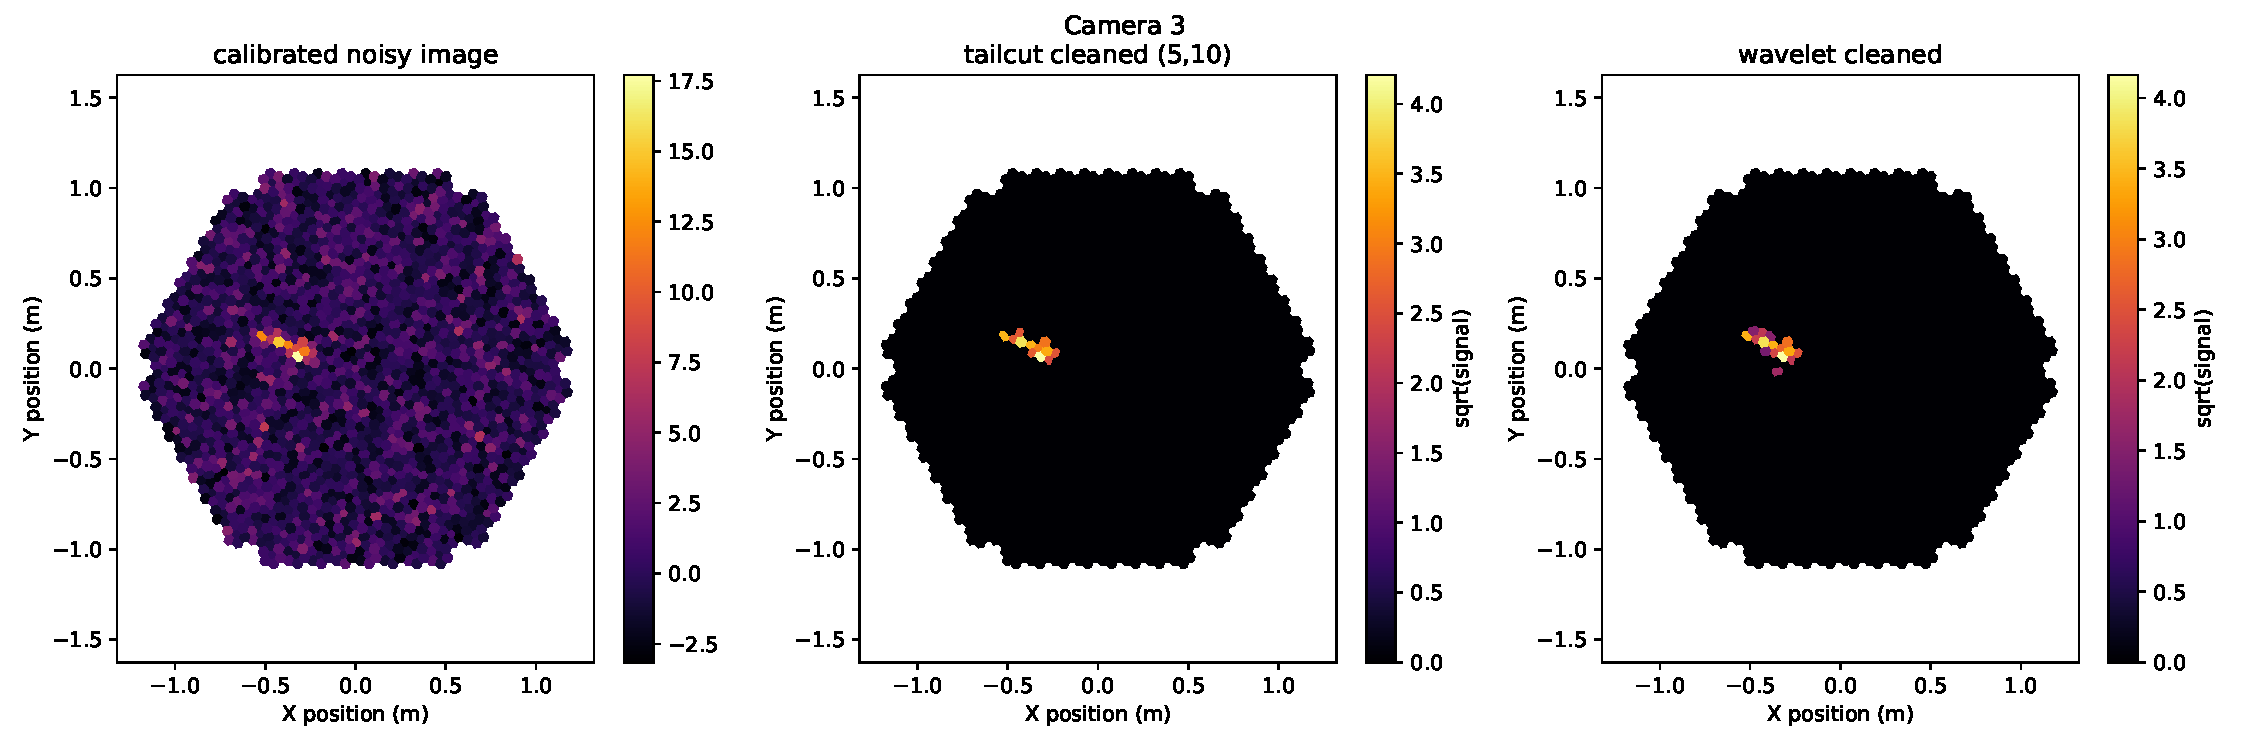
\includegraphics[width=\textwidth]{pics/camera_display_cleaning}
    \end{frame}



    \begin{frame}{Shower Reconstruction -- Direction}
            {Angle between reconstructed and simulated direction}
        \setlength{\figureheight}{4.5cm}
        \setlength{\figurewidth}{10cm}
        \centering
        % This file was created by matplotlib2tikz v0.6.13.
\begin{tikzpicture}

\definecolor{color0}{rgb}{1,0.549019607843137,0}

\begin{groupplot}[group style={group size=1 by 2}]
\nextgroupplot[
title={angular resolution},
% xlabel={$E_\mathrm{reco}$ / TeV},
ylabel={$\xi_\mathrm{68} / ^\circ$},
xmin=0.01, xmax=400,
ymin=0.0, ymax=.5,
xmode=log,
% ymode=log,
ytick={0.05,0.15,...,0.45},
width=\figurewidth,
height=\figureheight,
tick align=outside,
tick pos=left,
xmajorgrids,
x grid style={lightgray!92.026143790849673!black},
ymajorgrids,
y grid style={lightgray!92.026143790849673!black},
legend cell align={left},
legend style={at={(0.95,0.95)}, anchor=north east, draw=white!80.0!black},
legend entries={{gamma--tail},{gamma--wave}}
]
\addlegendimage{mark=square*, mark size=1.5, thick, color0}
\addlegendimage{mark=square*, mark size=1.5, thick, red!54.509803921568626!black}
\addplot [thick, color0, mark=square*, mark size=1.5, mark options={solid}]
table {%
0.0136454285810959 0.514373781681061
0.0235941156512618 0.379991948604584
0.0407962483594201 0.3049496114254
0.0705402103136033 0.237757019996643
0.121970070072348 0.1782096773386
0.210896705968349 0.142677937150002
0.364658481887548 0.120356653928757
0.630525772329928 0.112422074973583
1.09023310664374 0.109928931295872
1.88510649204695 0.099300679564476
3.25951070895043 0.083038901090622
5.63597340870963 0.0738796889781952
9.74508111799092 0.0794707235693932
16.8500805645153 0.0791967868804932
29.1352336212457 0.0727821743488312
50.3773162932047 0.0642204469442368
87.1066980240359 0.0649696215987206
150.614947340378 0.0348668572306633
260.42615409535 0.055004151314497
};
\addplot [thick, red!54.509803921568626!black, mark=square*, mark size=1.5, mark options={solid}]
table {%
0.0136454285810959 0.732811511844338
0.0235941156512618 0.579904953713132
0.0407962483594201 0.364272133170011
0.0705402103136033 0.23034186712471
0.121970070072348 0.142863084392569
0.210896705968349 0.10738983880055
0.364658481887548 0.0846159119918269
0.630525772329928 0.0819307208286604
1.09023310664374 0.0914241467604887
1.88510649204695 0.0841599381915339
3.25951070895043 0.0673358920970343
5.63597340870963 0.0579409335768772
9.74508111799092 0.0504428647595875
16.8500805645153 0.0433242364598634
29.1352336212457 0.0420815615661116
50.3773162932047 0.0370338122863349
87.1066980240359 0.04192093617672
150.614947340378 0.0253178552824584
260.42615409535 0.0294376533224965
};

\nextgroupplot[
xlabel={$\log_{10}(E_\mathrm{reco}$ / TeV)},
ytick={0.6,1,...,1.8},
ylabel={ratio},
xmin=0.01, xmax=400,
ymin=0.594604384534327, ymax=1.92915799774866,
xmode=log,
xmajorgrids,
ymajorgrids,
width=\figurewidth,
height=.8\figureheight,
tick align=outside,
tick pos=left,
x grid style={lightgray!92.026143790849673!black},
y grid style={lightgray!92.026143790849673!black}
]
\addplot [thick, darkred, forget plot]
table {%
0.0136454285810959 0.701918260517615
0.0235941156512618 0.655265912407706
0.0407962483594201 0.837147790503852
0.0705402103136033 1.03219194566969
0.121970070072348 1.24741586041152
0.210896705968349 1.32859811266678
0.364658481887548 1.42238795393923
0.630525772329928 1.37216020848503
1.09023310664374 1.2024058762491
1.88510649204695 1.17990437847619
3.25951070895043 1.23320414276177
5.63597340870963 1.27508627178349
9.74508111799092 1.57546015572576
16.8500805645153 1.82800190728954
29.1352336212457 1.72955022675401
50.3773162932047 1.7341030528454
87.1066980240359 1.54981323233903
150.614947340378 1.37716472590871
260.42615409535 1.86849646987528
};
\addplot [thick, darkorange, forget plot]
table {%
0.0136454285810959 1
0.0235941156512618 1
0.0407962483594201 1
0.0705402103136033 1
0.121970070072348 1
0.210896705968349 1
0.364658481887548 1
0.630525772329928 1
1.09023310664374 1
1.88510649204695 1
3.25951070895043 1
5.63597340870963 1
9.74508111799092 1
16.8500805645153 1
29.1352336212457 1
50.3773162932047 1
87.1066980240359 1
150.614947340378 1
260.42615409535 1
};


\end{groupplot}

\end{tikzpicture}

    \end{frame}




    \begin{frame}{Shower Reconstruction -- Shower Energy}
                 {Machine learning}
        \begin{itemize}
            \item train 1 Random Decision Forest for each telescope type
            \item follow a telescope-by-telescope approach
            \medskip
            \item then, for a given shower event, let the Forest estimate the energy from
                every telescope separately and combine them into a single energy
                estimator
        \end{itemize}
        \setlength{\figureheight}{4.5cm}
        \setlength{\figurewidth}{4.5cm}
        % This file was created by matplotlib2tikz v0.6.13.
\begin{tikzpicture}

\begin{groupplot}[group style={group size=3 by 1}]
\nextgroupplot[
title={gamma},
xlabel={$E_\mathrm{reco}$ / TeV},
ylabel={$E_\mathrm{MC}$ / TeV},
xmin=0.01, xmax=316.227766016838,
ymin=0.01, ymax=316.227766016838,
xmode=log,
ymode=log,
width=\figurewidth,
height=\figureheight,
tick align=outside,
tick pos=left,
xmajorgrids,
x grid style={lightgray!92.026143790849673!black},
ymajorgrids,
y grid style={lightgray!92.026143790849673!black}
]
\addplot graphics [includegraphics cmd=\pgfimage,xmin=0.01, xmax=316.227766016838, ymin=0.01, ymax=316.227766016838] {\detokenize{pics/energy_migration_wavelets_img000.png}};
\addplot [semithick, green!39.215686274509807!black, forget plot]
table {%
0.01 0.01
316.227766016838 316.227766016838
};
\nextgroupplot[
title={proton},
xlabel={$E_\mathrm{reco}$ / TeV},
xmin=0.01, xmax=316.227766016838,
ymin=0.01, ymax=316.227766016838,
xmode=log,
ymode=log,
width=\figurewidth,
height=\figureheight,
tick align=outside,
tick pos=left,
xmajorgrids,
x grid style={lightgray!92.026143790849673!black},
ymajorgrids,
y grid style={lightgray!92.026143790849673!black}
]
\addplot graphics [includegraphics cmd=\pgfimage,xmin=0.01, xmax=316.227766016838, ymin=0.01, ymax=316.227766016838] {\detokenize{pics/energy_migration_wavelets_img001.png}};
\addplot [semithick, green!39.215686274509807!black, forget plot]
table {%
0.01 0.01
316.227766016838 316.227766016838
};
\nextgroupplot[
title={electron},
xlabel={$E_\mathrm{reco}$ / TeV},
xmin=0.01, xmax=316.227766016838,
ymin=0.01, ymax=316.227766016838,
xmode=log,
ymode=log,
width=\figurewidth,
height=\figureheight,
tick align=outside,
tick pos=left,
xmajorgrids,
x grid style={lightgray!92.026143790849673!black},
ymajorgrids,
y grid style={lightgray!92.026143790849673!black}
]
\addplot graphics [includegraphics cmd=\pgfimage,xmin=0.01, xmax=316.227766016838, ymin=0.01, ymax=316.227766016838] {\detokenize{pics/energy_migration_wavelets_img002.png}};
\addplot [semithick, green!39.215686274509807!black, forget plot]
table {%
0.01 0.01
316.227766016838 316.227766016838
};
\end{groupplot}


\end{tikzpicture}

    \end{frame}


    \begin{frame}{Shower Reconstruction -- Shower Energy}
        \setlength{\figureheight}{4.cm}
        \setlength{\figurewidth}{4.5cm}
        % This file was created by matplotlib2tikz v0.6.13.
\begin{tikzpicture}

\begin{groupplot}[group style={group size=3 by 1}]
\nextgroupplot[
title={gamma},
xlabel={$E_\mathrm{reco}$ / TeV},
ylabel={$(E_\mathrm{reco} - E_\mathrm{MC})$ / TeV},
xmin=0.01, xmax=316.227766016838,
ymin=-1, ymax=1,
xmode=log,
width=\figurewidth,
height=\figureheight,
tick align=outside,
tick pos=left,
xmajorgrids,
x grid style={lightgray!92.026143790849673!black},
ymajorgrids,
y grid style={lightgray!92.026143790849673!black}
]
\addplot graphics [includegraphics cmd=\pgfimage,xmin=0.01, xmax=316.227766016838, ymin=-1, ymax=1] {\detokenize{pics/DeltaE_vs_recoE_wavelets_img000.png}};
\addplot [semithick, green!39.215686274509807!black, forget plot]
table {%
0.01 0
316.227766016838 0
};
\nextgroupplot[
title={proton},
xlabel={$E_\mathrm{reco}$ / TeV},
xmin=0.01, xmax=316.227766016838,
ymin=-1, ymax=1,
xmode=log,
width=\figurewidth,
height=\figureheight,
tick align=outside,
tick pos=left,
xmajorgrids,
x grid style={lightgray!92.026143790849673!black},
ymajorgrids,
y grid style={lightgray!92.026143790849673!black}
]
\addplot graphics [includegraphics cmd=\pgfimage,xmin=0.01, xmax=316.227766016838, ymin=-1, ymax=1] {\detokenize{pics/DeltaE_vs_recoE_wavelets_img001.png}};
\addplot [semithick, green!39.215686274509807!black, forget plot]
table {%
0.01 0
316.227766016838 0
};
\nextgroupplot[
title={electron},
xlabel={$E_\mathrm{reco}$ / TeV},
xmin=0.01, xmax=316.227766016838,
ymin=-1, ymax=1,
xmode=log,
width=\figurewidth,
height=\figureheight,
tick align=outside,
tick pos=left,
xmajorgrids,
x grid style={lightgray!92.026143790849673!black},
ymajorgrids,
y grid style={lightgray!92.026143790849673!black}
]
\addplot graphics [includegraphics cmd=\pgfimage,xmin=0.01, xmax=316.227766016838, ymin=-1, ymax=1] {\detokenize{pics/DeltaE_vs_recoE_wavelets_img002.png}};
\addplot [semithick, green!39.215686274509807!black, forget plot]
table {%
0.01 0
316.227766016838 0
};
\end{groupplot}

\end{tikzpicture}
\\
        \begin{columns}
            \setlength{\figurewidth}{.5\textwidth}
            \column{.5\textwidth}
                % This file was created by matplotlib2tikz v0.6.13.
\begin{tikzpicture}

\definecolor{color0}{rgb}{1,0.549019607843137,0}

\begin{axis}[
title={Energy Resolution},
xlabel={$E_\mathrm{reco}$ / TeV},
ylabel={$(|E_\mathrm{reco} - E_\mathrm{MC}|)_{68}/E_\mathrm{reco}$},
xmin=0.00833589642646998, xmax=426.304059521818,
ymin=0.144091539919376, ymax=0.733744545638562,
xmode=log,
width=\figurewidth,
height=\figureheight,
tick align=outside,
tick pos=left,
xmajorgrids,
x grid style={lightgray!92.026143790849673!black},
ymajorgrids,
y grid style={lightgray!92.026143790849673!black},
legend entries={{gamma -- tail},{gamma -- wave}},
legend style={at={(0.03,0.97)}, anchor=north west, draw=white!80.0!black},
legend cell align={left}
]
\addlegendimage{thick, mark=square*, mark size=1, color0}
\addlegendimage{thick, mark=square*, mark size=1, red!54.509803921568626!black}
\addplot [thick, color0, mark=square*, mark size=1, mark options={solid}]
table {%
0.0136454285810959 0.421641379594803
0.0235941156512618 0.357527391910553
0.0407962483594201 0.297841341495514
0.0705402103136033 0.274738141298294
0.121970070072348 0.227736700773239
0.210896705968349 0.198233005404472
0.364658481887548 0.225156680345535
0.630525772329928 0.221404126286507
1.09023310664374 0.2205261105299
1.88510649204695 0.207844513654709
3.25951070895043 0.209677596092224
5.63597340870963 0.230805432796478
9.74508111799092 0.250905712842941
16.8500805645153 0.290091704130173
29.1352336212457 0.342706776857376
50.3773162932047 0.428261777162552
87.1066980240359 0.70694213628769
150.614947340378 0.506991288661957
260.42615409535 0.516227679252625
};
\addplot [thick, red!54.509803921568626!black, mark=square*, mark size=1, mark options={solid}]
table {%
0.0136454285810959 0.409451516866684
0.0235941156512618 0.350892677307129
0.0407962483594201 0.278645443916321
0.0705402103136033 0.243579407334328
0.121970070072348 0.189551951885223
0.210896705968349 0.17393575489521
0.364658481887548 0.201668537259102
0.630525772329928 0.195855206251144
1.09023310664374 0.184799203872681
1.88510649204695 0.170893949270248
3.25951070895043 0.172493520975113
5.63597340870963 0.192388534545899
9.74508111799092 0.221660990715027
16.8500805645153 0.258518153429031
29.1352336212457 0.307165206670761
50.3773162932047 0.345951037406921
87.1066980240359 0.566645002365112
150.614947340378 0.560816395282745
260.42615409535 0.539847106933594
};
\end{axis}

\end{tikzpicture}

            \column{.5\textwidth}
                % This file was created by matplotlib2tikz v0.6.13.
\begin{tikzpicture}

\definecolor{color0}{rgb}{1,0.549019607843137,0}

\begin{axis}[
title={Energy Bias},
xlabel={$E_\mathrm{reco}$ / TeV},
ylabel={$(1 - E_\mathrm{reco}/E_\mathrm{MC})_{50}$},
ytick={-0.2,-0.1,0,0.1,0.2},
xmin=0.00833589642646998, xmax=426.304059521818,
ymin=-0.2, ymax=0.3,
xmode=log,
width=\figurewidth,
height=\figureheight,
tick align=outside,
tick pos=left,
xmajorgrids,
x grid style={lightgray!92.026143790849673!black},
ymajorgrids,
y grid style={lightgray!92.026143790849673!black},
legend entries={{gamma -- wavelets},{gamma -- tailcuts}},
legend style={at={(0.03,0.97)}, anchor=north west, draw=white!80.0!black},
legend cell align={left}
]
\addlegendimage{thick,mark=square*, mark size=1, red!54.509803921568626!black}
\addlegendimage{thick,mark=square*, mark size=1, color0}
\addplot [thick, red!54.509803921568626!black, mark=square*, mark size=1, mark options={solid}]
table {%
0.0136454285810959 -0.0921624302864075
0.0235941156512618 -0.0915325284004211
0.0407962483594201 -0.0790250301361084
0.0705402103136033 -0.0913239717483521
0.121970070072348 -0.0275206565856934
0.210896705968349 -0.014256477355957
0.364658481887548 -0.0453824996948242
0.630525772329928 -0.0458172559738159
1.09023310664374 -0.0451393723487854
1.88510649204695 -0.0257483720779419
3.25951070895043 -0.0137485861778259
5.63597340870963 -0.010492742061615
9.74508111799092 -0.0420072674751282
16.8500805645153 -0.0491601228713989
29.1352336212457 -0.0389223098754883
50.3773162932047 -0.024517297744751
87.1066980240359 0.192897975444794
150.614947340378 0.104785025119781
260.42615409535 -0.476514220237732
};
\addplot [thick, color0, mark=square*, mark size=1, mark options={solid}]
table {%
0.0136454285810959 -0.0966137051582336
0.0235941156512618 -0.0917153358459473
0.0407962483594201 -0.0679131746292114
0.0705402103136033 -0.0968486070632935
0.121970070072348 -0.0446124076843262
0.210896705968349 -0.0177986621856689
0.364658481887548 -0.0549615025520325
0.630525772329928 -0.0590299367904663
1.09023310664374 -0.0741158723831177
1.88510649204695 -0.051228404045105
3.25951070895043 -0.0388984680175781
5.63597340870963 -0.0395519733428955
9.74508111799092 -0.0618356466293335
16.8500805645153 -0.0684826374053955
29.1352336212457 -0.0452133417129517
50.3773162932047 0.0244642496109009
87.1066980240359 0.207014441490173
150.614947340378 -0.0489252805709839
260.42615409535 -0.480178356170654
};
\end{axis}

\end{tikzpicture}

        \end{columns}
    \end{frame}



    \begin{frame}{Next Stop: Event Classification}
        \setlength{\figureheight}{4.cm}
        \setlength{\figurewidth}{4.5cm}
        \begin{columns}
            \column{.33\textwidth}
                % This file was created by matplotlib2tikz v0.6.13.
\begin{tikzpicture}

\definecolor{color0}{rgb}{1,0.647058823529412,0}

\begin{axis}[
xlabel={gammaness},
ylabel={normalised Events},
xmin=0., xmax=1.0,
ymin=0, ymax=37.480405349055,
width=\figurewidth,
height=\figureheight,
tick align=outside,
tick pos=left,
x grid style={lightgray!92.026143790849673!black},
y grid style={lightgray!92.026143790849673!black},
% legend entries={{integral normalised},{gamma--wavelets},{proton--wavelets},
% {electron--wavelets}},
% legend style={at={(0.03,0.97)}, anchor=north west, draw=white!80.0!black},
% legend cell align={left}
]
\addlegendimage{empty legend}
\addlegendimage{ybar,ybar legend,fill=color0,draw opacity=0,fill opacity=0.5};
\draw[fill=color0,draw opacity=0,fill opacity=0.5] (axis cs:0,0) rectangle (axis cs:0.01,0.126140314861623);
\draw[fill=color0,draw opacity=0,fill opacity=0.5] (axis cs:0.01,0) rectangle (axis cs:0.02,0.109059649212846);
\draw[fill=color0,draw opacity=0,fill opacity=0.5] (axis cs:0.02,0) rectangle (axis cs:0.03,0.111946522280245);
\draw[fill=color0,draw opacity=0,fill opacity=0.5] (axis cs:0.03,0) rectangle (axis cs:0.04,0.109540794724079);
\draw[fill=color0,draw opacity=0,fill opacity=0.5] (axis cs:0.04,0) rectangle (axis cs:0.05,0.114913586266183);
\draw[fill=color0,draw opacity=0,fill opacity=0.5] (axis cs:0.05,0) rectangle (axis cs:0.06,0.12349401454984);
\draw[fill=color0,draw opacity=0,fill opacity=0.5] (axis cs:0.06,0) rectangle (axis cs:0.07,0.120045805052669);
\draw[fill=color0,draw opacity=0,fill opacity=0.5] (axis cs:0.07,0) rectangle (axis cs:0.08,0.138008570805374);
\draw[fill=color0,draw opacity=0,fill opacity=0.5] (axis cs:0.08,0) rectangle (axis cs:0.09,0.131513106403726);
\draw[fill=color0,draw opacity=0,fill opacity=0.5] (axis cs:0.09,0) rectangle (axis cs:0.1,0.137286852538523);
\draw[fill=color0,draw opacity=0,fill opacity=0.5] (axis cs:0.1,0) rectangle (axis cs:0.11,0.161584700855798);
\draw[fill=color0,draw opacity=0,fill opacity=0.5] (axis cs:0.11,0) rectangle (axis cs:0.12,0.164471573923197);
\draw[fill=color0,draw opacity=0,fill opacity=0.5] (axis cs:0.12,0) rectangle (axis cs:0.13,0.154207136350222);
\draw[fill=color0,draw opacity=0,fill opacity=0.5] (axis cs:0.13,0) rectangle (axis cs:0.14,0.177061548133797);
\draw[fill=color0,draw opacity=0,fill opacity=0.5] (axis cs:0.14,0) rectangle (axis cs:0.15,0.185160830906222);
\draw[fill=color0,draw opacity=0,fill opacity=0.5] (axis cs:0.15,0) rectangle (axis cs:0.16,0.161825273611414);
\draw[fill=color0,draw opacity=0,fill opacity=0.5] (axis cs:0.16,0) rectangle (axis cs:0.17,0.195345077560656);
\draw[fill=color0,draw opacity=0,fill opacity=0.5] (axis cs:0.17,0) rectangle (axis cs:0.18,0.171849138428772);
\draw[fill=color0,draw opacity=0,fill opacity=0.5] (axis cs:0.18,0) rectangle (axis cs:0.19,0.187967513055081);
\draw[fill=color0,draw opacity=0,fill opacity=0.5] (axis cs:0.19,0) rectangle (axis cs:0.2,0.198151759709516);
\draw[fill=color0,draw opacity=0,fill opacity=0.5] (axis cs:0.2,0) rectangle (axis cs:0.21,0.17617944802987);
\draw[fill=color0,draw opacity=0,fill opacity=0.5] (axis cs:0.21,0) rectangle (axis cs:0.22,0.193741259189879);
\draw[fill=color0,draw opacity=0,fill opacity=0.5] (axis cs:0.22,0) rectangle (axis cs:0.23,0.180028612119734);
\draw[fill=color0,draw opacity=0,fill opacity=0.5] (axis cs:0.23,0) rectangle (axis cs:0.24,0.217237198321765);
\draw[fill=color0,draw opacity=0,fill opacity=0.5] (axis cs:0.24,0) rectangle (axis cs:0.25,0.187726940299465);
\draw[fill=color0,draw opacity=0,fill opacity=0.5] (axis cs:0.25,0) rectangle (axis cs:0.26,0.195345077560656);
\draw[fill=color0,draw opacity=0,fill opacity=0.5] (axis cs:0.26,0) rectangle (axis cs:0.27,0.182354148757361);
\draw[fill=color0,draw opacity=0,fill opacity=0.5] (axis cs:0.27,0) rectangle (axis cs:0.28,0.225577053849805);
\draw[fill=color0,draw opacity=0,fill opacity=0.5] (axis cs:0.28,0) rectangle (axis cs:0.29,0.202722642066233);
\draw[fill=color0,draw opacity=0,fill opacity=0.5] (axis cs:0.29,0) rectangle (axis cs:0.3,0.212666315965049);
\draw[fill=color0,draw opacity=0,fill opacity=0.5] (axis cs:0.3,0) rectangle (axis cs:0.31,0.197109277768511);
\draw[fill=color0,draw opacity=0,fill opacity=0.5] (axis cs:0.31,0) rectangle (axis cs:0.32,0.233355572948074);
\draw[fill=color0,draw opacity=0,fill opacity=0.5] (axis cs:0.32,0) rectangle (axis cs:0.33,0.214350325254365);
\draw[fill=color0,draw opacity=0,fill opacity=0.5] (axis cs:0.33,0) rectangle (axis cs:0.34,0.219963689552085);
\draw[fill=color0,draw opacity=0,fill opacity=0.5] (axis cs:0.34,0) rectangle (axis cs:0.35,0.223411899049256);
\draw[fill=color0,draw opacity=0,fill opacity=0.5] (axis cs:0.35,0) rectangle (axis cs:0.36,0.212345552290896);
\draw[fill=color0,draw opacity=0,fill opacity=0.5] (axis cs:0.36,0) rectangle (axis cs:0.37,0.272087786602342);
\draw[fill=color0,draw opacity=0,fill opacity=0.5] (axis cs:0.37,0) rectangle (axis cs:0.38,0.243058674091276);
\draw[fill=color0,draw opacity=0,fill opacity=0.5] (axis cs:0.38,0) rectangle (axis cs:0.39,0.250917384108084);
\draw[fill=color0,draw opacity=0,fill opacity=0.5] (axis cs:0.39,0) rectangle (axis cs:0.4,0.242497337661504);
\draw[fill=color0,draw opacity=0,fill opacity=0.5] (axis cs:0.4,0) rectangle (axis cs:0.41,0.302480144728569);
\draw[fill=color0,draw opacity=0,fill opacity=0.5] (axis cs:0.41,0) rectangle (axis cs:0.42,0.283956042546096);
\draw[fill=color0,draw opacity=0,fill opacity=0.5] (axis cs:0.42,0) rectangle (axis cs:0.43,0.283555087953399);
\draw[fill=color0,draw opacity=0,fill opacity=0.5] (axis cs:0.43,0) rectangle (axis cs:0.44,0.290130743273585);
\draw[fill=color0,draw opacity=0,fill opacity=0.5] (axis cs:0.44,0) rectangle (axis cs:0.45,0.290371316029202);
\draw[fill=color0,draw opacity=0,fill opacity=0.5] (axis cs:0.45,0) rectangle (axis cs:0.46,0.358453405868692);
\draw[fill=color0,draw opacity=0,fill opacity=0.5] (axis cs:0.46,0) rectangle (axis cs:0.47,0.324292074571138);
\draw[fill=color0,draw opacity=0,fill opacity=0.5] (axis cs:0.47,0) rectangle (axis cs:0.48,0.336320712351971);
\draw[fill=color0,draw opacity=0,fill opacity=0.5] (axis cs:0.48,0) rectangle (axis cs:0.49,0.333834793877262);
\draw[fill=color0,draw opacity=0,fill opacity=0.5] (axis cs:0.49,0) rectangle (axis cs:0.5,0.327178947638537);
\draw[fill=color0,draw opacity=0,fill opacity=0.5] (axis cs:0.5,0) rectangle (axis cs:0.51,0.429502559694119);
\draw[fill=color0,draw opacity=0,fill opacity=0.5] (axis cs:0.51,0) rectangle (axis cs:0.52,0.380586099385416);
\draw[fill=color0,draw opacity=0,fill opacity=0.5] (axis cs:0.52,0) rectangle (axis cs:0.53,0.386199463683136);
\draw[fill=color0,draw opacity=0,fill opacity=0.5] (axis cs:0.53,0) rectangle (axis cs:0.54,0.392775119003322);
\draw[fill=color0,draw opacity=0,fill opacity=0.5] (axis cs:0.54,0) rectangle (axis cs:0.55,0.46663095497761);
\draw[fill=color0,draw opacity=0,fill opacity=0.5] (axis cs:0.55,0) rectangle (axis cs:0.56,0.42380900447786);
\draw[fill=color0,draw opacity=0,fill opacity=0.5] (axis cs:0.56,0) rectangle (axis cs:0.57,0.442974634008647);
\draw[fill=color0,draw opacity=0,fill opacity=0.5] (axis cs:0.57,0) rectangle (axis cs:0.58,0.438644324407558);
\draw[fill=color0,draw opacity=0,fill opacity=0.5] (axis cs:0.58,0) rectangle (axis cs:0.59,0.43575745134015);
\draw[fill=color0,draw opacity=0,fill opacity=0.5] (axis cs:0.59,0) rectangle (axis cs:0.6,0.541930227485597);
\draw[fill=color0,draw opacity=0,fill opacity=0.5] (axis cs:0.6,0) rectangle (axis cs:0.61,0.500070568008313);
\draw[fill=color0,draw opacity=0,fill opacity=0.5] (axis cs:0.61,0) rectangle (axis cs:0.62,0.503518777505484);
\draw[fill=color0,draw opacity=0,fill opacity=0.5] (axis cs:0.62,0) rectangle (axis cs:0.63,0.507047177921194);
\draw[fill=color0,draw opacity=0,fill opacity=0.5] (axis cs:0.63,0) rectangle (axis cs:0.64,0.593492988106082);
\draw[fill=color0,draw opacity=0,fill opacity=0.5] (axis cs:0.64,0) rectangle (axis cs:0.65,0.526453380207597);
\draw[fill=color0,draw opacity=0,fill opacity=0.5] (axis cs:0.65,0) rectangle (axis cs:0.66,0.566308266721409);
\draw[fill=color0,draw opacity=0,fill opacity=0.5] (axis cs:0.66,0) rectangle (axis cs:0.67,0.580582250221326);
\draw[fill=color0,draw opacity=0,fill opacity=0.5] (axis cs:0.67,0) rectangle (axis cs:0.68,0.568072466929264);
\draw[fill=color0,draw opacity=0,fill opacity=0.5] (axis cs:0.68,0) rectangle (axis cs:0.69,0.693491063524037);
\draw[fill=color0,draw opacity=0,fill opacity=0.5] (axis cs:0.69,0) rectangle (axis cs:0.7,0.6189135092829);
\draw[fill=color0,draw opacity=0,fill opacity=0.5] (axis cs:0.7,0) rectangle (axis cs:0.71,0.653155031499006);
\draw[fill=color0,draw opacity=0,fill opacity=0.5] (axis cs:0.71,0) rectangle (axis cs:0.72,0.636074365850215);
\draw[fill=color0,draw opacity=0,fill opacity=0.5] (axis cs:0.72,0) rectangle (axis cs:0.73,0.752671961405713);
\draw[fill=color0,draw opacity=0,fill opacity=0.5] (axis cs:0.73,0) rectangle (axis cs:0.74,0.692528772501571);
\draw[fill=color0,draw opacity=0,fill opacity=0.5] (axis cs:0.74,0) rectangle (axis cs:0.75,0.723642848894647);
\draw[fill=color0,draw opacity=0,fill opacity=0.5] (axis cs:0.75,0) rectangle (axis cs:0.76,0.725888194613735);
\draw[fill=color0,draw opacity=0,fill opacity=0.5] (axis cs:0.76,0) rectangle (axis cs:0.77,0.848500109059648);
\draw[fill=color0,draw opacity=0,fill opacity=0.5] (axis cs:0.77,0) rectangle (axis cs:0.78,0.793890093534686);
\draw[fill=color0,draw opacity=0,fill opacity=0.5] (axis cs:0.78,0) rectangle (axis cs:0.79,0.847457627118643);
\draw[fill=color0,draw opacity=0,fill opacity=0.5] (axis cs:0.79,0) rectangle (axis cs:0.8,0.823159778801369);
\draw[fill=color0,draw opacity=0,fill opacity=0.5] (axis cs:0.8,0) rectangle (axis cs:0.81,0.961248540525281);
\draw[fill=color0,draw opacity=0,fill opacity=0.5] (axis cs:0.81,0) rectangle (axis cs:0.82,0.944248065795043);
\draw[fill=color0,draw opacity=0,fill opacity=0.5] (axis cs:0.82,0) rectangle (axis cs:0.83,0.971031832587022);
\draw[fill=color0,draw opacity=0,fill opacity=0.5] (axis cs:0.83,0) rectangle (axis cs:0.84,1.11409243126037);
\draw[fill=color0,draw opacity=0,fill opacity=0.5] (axis cs:0.84,0) rectangle (axis cs:0.85,1.05988337032808);
\draw[fill=color0,draw opacity=0,fill opacity=0.5] (axis cs:0.85,0) rectangle (axis cs:0.86,1.16886282862238);
\draw[fill=color0,draw opacity=0,fill opacity=0.5] (axis cs:0.86,0) rectangle (axis cs:0.87,1.30462605370867);
\draw[fill=color0,draw opacity=0,fill opacity=0.5] (axis cs:0.87,0) rectangle (axis cs:0.88,1.2209067347541);
\draw[fill=color0,draw opacity=0,fill opacity=0.5] (axis cs:0.88,0) rectangle (axis cs:0.89,1.37864227152003);
\draw[fill=color0,draw opacity=0,fill opacity=0.5] (axis cs:0.89,0) rectangle (axis cs:0.9,1.52659451622422);
\draw[fill=color0,draw opacity=0,fill opacity=0.5] (axis cs:0.9,0) rectangle (axis cs:0.91,1.52330668856413);
\draw[fill=color0,draw opacity=0,fill opacity=0.5] (axis cs:0.91,0) rectangle (axis cs:0.92,1.61071478977149);
\draw[fill=color0,draw opacity=0,fill opacity=0.5] (axis cs:0.92,0) rectangle (axis cs:0.93,1.82835294268594);
\draw[fill=color0,draw opacity=0,fill opacity=0.5] (axis cs:0.93,0) rectangle (axis cs:0.94,1.97117296860365);
\draw[fill=color0,draw opacity=0,fill opacity=0.5] (axis cs:0.94,0) rectangle (axis cs:0.95,2.24085502764982);
\draw[fill=color0,draw opacity=0,fill opacity=0.5] (axis cs:0.95,0) rectangle (axis cs:0.96,2.56121774721262);
\draw[fill=color0,draw opacity=0,fill opacity=0.5] (axis cs:0.96,0) rectangle (axis cs:0.97,2.93763391883396);
\draw[fill=color0,draw opacity=0,fill opacity=0.5] (axis cs:0.97,0) rectangle (axis cs:0.98,3.9016891415081);
\draw[fill=color0,draw opacity=0,fill opacity=0.5] (axis cs:0.98,0) rectangle (axis cs:0.99,6.19274368416325);
\draw[fill=color0,draw opacity=0,fill opacity=0.5] (axis cs:0.99,0) rectangle (axis cs:1,35.6956241419571);
\addlegendimage{ybar,ybar legend,fill=blue,draw opacity=0,fill opacity=0.5};
\draw[fill=blue,draw opacity=0,fill opacity=0.5] (axis cs:0,0) rectangle (axis cs:0.01,8.97831506407033);
\draw[fill=blue,draw opacity=0,fill opacity=0.5] (axis cs:0.01,0) rectangle (axis cs:0.02,5.2828251284847);
\draw[fill=blue,draw opacity=0,fill opacity=0.5] (axis cs:0.02,0) rectangle (axis cs:0.03,4.67626089672);
\draw[fill=blue,draw opacity=0,fill opacity=0.5] (axis cs:0.03,0) rectangle (axis cs:0.04,3.6676140924737);
\draw[fill=blue,draw opacity=0,fill opacity=0.5] (axis cs:0.04,0) rectangle (axis cs:0.05,3.53811492257396);
\draw[fill=blue,draw opacity=0,fill opacity=0.5] (axis cs:0.05,0) rectangle (axis cs:0.06,3.20519266971184);
\draw[fill=blue,draw opacity=0,fill opacity=0.5] (axis cs:0.06,0) rectangle (axis cs:0.07,2.37473954611776);
\draw[fill=blue,draw opacity=0,fill opacity=0.5] (axis cs:0.07,0) rectangle (axis cs:0.08,2.58274979313655);
\draw[fill=blue,draw opacity=0,fill opacity=0.5] (axis cs:0.08,0) rectangle (axis cs:0.09,1.85956573670737);
\draw[fill=blue,draw opacity=0,fill opacity=0.5] (axis cs:0.09,0) rectangle (axis cs:0.1,1.86997507052764);
\draw[fill=blue,draw opacity=0,fill opacity=0.5] (axis cs:0.1,0) rectangle (axis cs:0.11,1.926961762459);
\draw[fill=blue,draw opacity=0,fill opacity=0.5] (axis cs:0.11,0) rectangle (axis cs:0.12,1.56792796035279);
\draw[fill=blue,draw opacity=0,fill opacity=0.5] (axis cs:0.12,0) rectangle (axis cs:0.13,1.50194336969543);
\draw[fill=blue,draw opacity=0,fill opacity=0.5] (axis cs:0.13,0) rectangle (axis cs:0.14,1.55557790327788);
\draw[fill=blue,draw opacity=0,fill opacity=0.5] (axis cs:0.14,0) rectangle (axis cs:0.15,1.29869671611983);
\draw[fill=blue,draw opacity=0,fill opacity=0.5] (axis cs:0.15,0) rectangle (axis cs:0.16,1.27964234234711);
\draw[fill=blue,draw opacity=0,fill opacity=0.5] (axis cs:0.16,0) rectangle (axis cs:0.17,1.34121619833486);
\draw[fill=blue,draw opacity=0,fill opacity=0.5] (axis cs:0.17,0) rectangle (axis cs:0.18,1.11521015386407);
\draw[fill=blue,draw opacity=0,fill opacity=0.5] (axis cs:0.18,0) rectangle (axis cs:0.19,1.07886570018648);
\draw[fill=blue,draw opacity=0,fill opacity=0.5] (axis cs:0.19,0) rectangle (axis cs:0.2,1.20607128805802);
\draw[fill=blue,draw opacity=0,fill opacity=0.5] (axis cs:0.2,0) rectangle (axis cs:0.21,0.884440515950102);
\draw[fill=blue,draw opacity=0,fill opacity=0.5] (axis cs:0.21,0) rectangle (axis cs:0.22,0.903318460336026);
\draw[fill=blue,draw opacity=0,fill opacity=0.5] (axis cs:0.22,0) rectangle (axis cs:0.23,0.876677622931584);
\draw[fill=blue,draw opacity=0,fill opacity=0.5] (axis cs:0.23,0) rectangle (axis cs:0.24,0.997002464718537);
\draw[fill=blue,draw opacity=0,fill opacity=0.5] (axis cs:0.24,0) rectangle (axis cs:0.25,0.717185457278505);
\draw[fill=blue,draw opacity=0,fill opacity=0.5] (axis cs:0.25,0) rectangle (axis cs:0.26,0.764821391710287);
\draw[fill=blue,draw opacity=0,fill opacity=0.5] (axis cs:0.26,0) rectangle (axis cs:0.27,0.71859689237278);
\draw[fill=blue,draw opacity=0,fill opacity=0.5] (axis cs:0.27,0) rectangle (axis cs:0.28,0.821808083641642);
\draw[fill=blue,draw opacity=0,fill opacity=0.5] (axis cs:0.28,0) rectangle (axis cs:0.29,0.624912887990281);
\draw[fill=blue,draw opacity=0,fill opacity=0.5] (axis cs:0.29,0) rectangle (axis cs:0.3,0.642202967895143);
\draw[fill=blue,draw opacity=0,fill opacity=0.5] (axis cs:0.3,0) rectangle (axis cs:0.31,0.621384300254587);
\draw[fill=blue,draw opacity=0,fill opacity=0.5] (axis cs:0.31,0) rectangle (axis cs:0.32,0.705893976524305);
\draw[fill=blue,draw opacity=0,fill opacity=0.5] (axis cs:0.32,0) rectangle (axis cs:0.33,0.537403912145222);
\draw[fill=blue,draw opacity=0,fill opacity=0.5] (axis cs:0.33,0) rectangle (axis cs:0.34,0.555928997757582);
\draw[fill=blue,draw opacity=0,fill opacity=0.5] (axis cs:0.34,0) rectangle (axis cs:0.35,0.541638217428047);
\draw[fill=blue,draw opacity=0,fill opacity=0.5] (axis cs:0.35,0) rectangle (axis cs:0.36,0.515526668183964);
\draw[fill=blue,draw opacity=0,fill opacity=0.5] (axis cs:0.36,0) rectangle (axis cs:0.37,0.608681384406111);
\draw[fill=blue,draw opacity=0,fill opacity=0.5] (axis cs:0.37,0) rectangle (axis cs:0.38,0.500177311533718);
\draw[fill=blue,draw opacity=0,fill opacity=0.5] (axis cs:0.38,0) rectangle (axis cs:0.39,0.494708000543402);
\draw[fill=blue,draw opacity=0,fill opacity=0.5] (axis cs:0.39,0) rectangle (axis cs:0.4,0.479005785119592);
\draw[fill=blue,draw opacity=0,fill opacity=0.5] (axis cs:0.4,0) rectangle (axis cs:0.41,0.565809043417507);
\draw[fill=blue,draw opacity=0,fill opacity=0.5] (axis cs:0.41,0) rectangle (axis cs:0.42,0.434898438423502);
\draw[fill=blue,draw opacity=0,fill opacity=0.5] (axis cs:0.42,0) rectangle (axis cs:0.43,0.467714304365392);
\draw[fill=blue,draw opacity=0,fill opacity=0.5] (axis cs:0.43,0) rectangle (axis cs:0.44,0.454305670969779);
\draw[fill=blue,draw opacity=0,fill opacity=0.5] (axis cs:0.44,0) rectangle (axis cs:0.45,0.444778484083422);
\draw[fill=blue,draw opacity=0,fill opacity=0.5] (axis cs:0.45,0) rectangle (axis cs:0.46,0.514820950636821);
\draw[fill=blue,draw opacity=0,fill opacity=0.5] (axis cs:0.46,0) rectangle (axis cs:0.47,0.424489104603218);
\draw[fill=blue,draw opacity=0,fill opacity=0.5] (axis cs:0.47,0) rectangle (axis cs:0.48,0.447248495498408);
\draw[fill=blue,draw opacity=0,fill opacity=0.5] (axis cs:0.48,0) rectangle (axis cs:0.49,0.442484902055225);
\draw[fill=blue,draw opacity=0,fill opacity=0.5] (axis cs:0.49,0) rectangle (axis cs:0.5,0.401906143094818);
\draw[fill=blue,draw opacity=0,fill opacity=0.5] (axis cs:0.5,0) rectangle (axis cs:0.51,0.508645922099368);
\draw[fill=blue,draw opacity=0,fill opacity=0.5] (axis cs:0.51,0) rectangle (axis cs:0.52,0.41972551116004);
\draw[fill=blue,draw opacity=0,fill opacity=0.5] (axis cs:0.52,0) rectangle (axis cs:0.53,0.439132743706322);
\draw[fill=blue,draw opacity=0,fill opacity=0.5] (axis cs:0.53,0) rectangle (axis cs:0.54,0.41972551116004);
\draw[fill=blue,draw opacity=0,fill opacity=0.5] (axis cs:0.54,0) rectangle (axis cs:0.55,0.488356542619164);
\draw[fill=blue,draw opacity=0,fill opacity=0.5] (axis cs:0.55,0) rectangle (axis cs:0.56,0.433839862102791);
\draw[fill=blue,draw opacity=0,fill opacity=0.5] (axis cs:0.56,0) rectangle (axis cs:0.57,0.442132043281656);
\draw[fill=blue,draw opacity=0,fill opacity=0.5] (axis cs:0.57,0) rectangle (axis cs:0.58,0.441955613894882);
\draw[fill=blue,draw opacity=0,fill opacity=0.5] (axis cs:0.58,0) rectangle (axis cs:0.59,0.413550482622587);
\draw[fill=blue,draw opacity=0,fill opacity=0.5] (axis cs:0.59,0) rectangle (axis cs:0.6,0.494002282996264);
\draw[fill=blue,draw opacity=0,fill opacity=0.5] (axis cs:0.6,0) rectangle (axis cs:0.61,0.450777083234091);
\draw[fill=blue,draw opacity=0,fill opacity=0.5] (axis cs:0.61,0) rectangle (axis cs:0.62,0.468596451299313);
\draw[fill=blue,draw opacity=0,fill opacity=0.5] (axis cs:0.62,0) rectangle (axis cs:0.63,0.447072066111619);
\draw[fill=blue,draw opacity=0,fill opacity=0.5] (axis cs:0.63,0) rectangle (axis cs:0.64,0.548166104739069);
\draw[fill=blue,draw opacity=0,fill opacity=0.5] (axis cs:0.64,0) rectangle (axis cs:0.65,0.466126439884332);
\draw[fill=blue,draw opacity=0,fill opacity=0.5] (axis cs:0.65,0) rectangle (axis cs:0.66,0.508998780872937);
\draw[fill=blue,draw opacity=0,fill opacity=0.5] (axis cs:0.66,0) rectangle (axis cs:0.67,0.50794020455223);
\draw[fill=blue,draw opacity=0,fill opacity=0.5] (axis cs:0.67,0) rectangle (axis cs:0.68,0.477065061864964);
\draw[fill=blue,draw opacity=0,fill opacity=0.5] (axis cs:0.68,0) rectangle (axis cs:0.69,0.599683485680108);
\draw[fill=blue,draw opacity=0,fill opacity=0.5] (axis cs:0.69,0) rectangle (axis cs:0.7,0.516055956344312);
\draw[fill=blue,draw opacity=0,fill opacity=0.5] (axis cs:0.7,0) rectangle (axis cs:0.71,0.555928997757594);
\draw[fill=blue,draw opacity=0,fill opacity=0.5] (axis cs:0.71,0) rectangle (axis cs:0.72,0.530876024834199);
\draw[fill=blue,draw opacity=0,fill opacity=0.5] (axis cs:0.72,0) rectangle (axis cs:0.73,0.633910786716278);
\draw[fill=blue,draw opacity=0,fill opacity=0.5] (axis cs:0.73,0) rectangle (axis cs:0.74,0.537227482758437);
\draw[fill=blue,draw opacity=0,fill opacity=0.5] (axis cs:0.74,0) rectangle (axis cs:0.75,0.603917790962933);
\draw[fill=blue,draw opacity=0,fill opacity=0.5] (axis cs:0.75,0) rectangle (axis cs:0.76,0.575689089077432);
\draw[fill=blue,draw opacity=0,fill opacity=0.5] (axis cs:0.76,0) rectangle (axis cs:0.77,0.69724893657187);
\draw[fill=blue,draw opacity=0,fill opacity=0.5] (axis cs:0.77,0) rectangle (axis cs:0.78,0.590685586954104);
\draw[fill=blue,draw opacity=0,fill opacity=0.5] (axis cs:0.78,0) rectangle (axis cs:0.79,0.655964460064325);
\draw[fill=blue,draw opacity=0,fill opacity=0.5] (axis cs:0.79,0) rectangle (axis cs:0.8,0.612386401528583);
\draw[fill=blue,draw opacity=0,fill opacity=0.5] (axis cs:0.8,0) rectangle (axis cs:0.81,0.724595491523449);
\draw[fill=blue,draw opacity=0,fill opacity=0.5] (axis cs:0.81,0) rectangle (axis cs:0.82,0.650142290300441);
\draw[fill=blue,draw opacity=0,fill opacity=0.5] (axis cs:0.82,0) rectangle (axis cs:0.83,0.646790131951537);
\draw[fill=blue,draw opacity=0,fill opacity=0.5] (axis cs:0.83,0) rectangle (axis cs:0.84,0.768173550059208);
\draw[fill=blue,draw opacity=0,fill opacity=0.5] (axis cs:0.84,0) rectangle (axis cs:0.85,0.627206470018471);
\draw[fill=blue,draw opacity=0,fill opacity=0.5] (axis cs:0.85,0) rectangle (axis cs:0.86,0.674842404450254);
\draw[fill=blue,draw opacity=0,fill opacity=0.5] (axis cs:0.86,0) rectangle (axis cs:0.87,0.752471334635381);
\draw[fill=blue,draw opacity=0,fill opacity=0.5] (axis cs:0.87,0) rectangle (axis cs:0.88,0.594567033463361);
\draw[fill=blue,draw opacity=0,fill opacity=0.5] (axis cs:0.88,0) rectangle (axis cs:0.89,0.669549522846722);
\draw[fill=blue,draw opacity=0,fill opacity=0.5] (axis cs:0.89,0) rectangle (axis cs:0.9,0.68031171544057);
\draw[fill=blue,draw opacity=0,fill opacity=0.5] (axis cs:0.9,0) rectangle (axis cs:0.91,0.60180063832152);
\draw[fill=blue,draw opacity=0,fill opacity=0.5] (axis cs:0.91,0) rectangle (axis cs:0.92,0.583804840869514);
\draw[fill=blue,draw opacity=0,fill opacity=0.5] (axis cs:0.92,0) rectangle (axis cs:0.93,0.611151395821093);
\draw[fill=blue,draw opacity=0,fill opacity=0.5] (axis cs:0.93,0) rectangle (axis cs:0.94,0.591214875114458);
\draw[fill=blue,draw opacity=0,fill opacity=0.5] (axis cs:0.94,0) rectangle (axis cs:0.95,0.577982671105629);
\draw[fill=blue,draw opacity=0,fill opacity=0.5] (axis cs:0.95,0) rectangle (axis cs:0.96,0.583628411482742);
\draw[fill=blue,draw opacity=0,fill opacity=0.5] (axis cs:0.96,0) rectangle (axis cs:0.97,0.573042648275666);
\draw[fill=blue,draw opacity=0,fill opacity=0.5] (axis cs:0.97,0) rectangle (axis cs:0.98,0.682958156242335);
\draw[fill=blue,draw opacity=0,fill opacity=0.5] (axis cs:0.98,0) rectangle (axis cs:0.99,0.87367832335625);
\draw[fill=blue,draw opacity=0,fill opacity=0.5] (axis cs:0.99,0) rectangle (axis cs:1,2.02946723618072);
\addlegendimage{ybar,ybar legend,fill=red,draw opacity=0,fill opacity=0.5};
\draw[fill=red,draw opacity=0,fill opacity=0.5] (axis cs:0,0) rectangle (axis cs:0.01,0.575932298570617);
\draw[fill=red,draw opacity=0,fill opacity=0.5] (axis cs:0.01,0) rectangle (axis cs:0.02,0.504756991831164);
\draw[fill=red,draw opacity=0,fill opacity=0.5] (axis cs:0.02,0) rectangle (axis cs:0.03,0.521081603468654);
\draw[fill=red,draw opacity=0,fill opacity=0.5] (axis cs:0.03,0) rectangle (axis cs:0.04,0.508674898624161);
\draw[fill=red,draw opacity=0,fill opacity=0.5] (axis cs:0.04,0) rectangle (axis cs:0.05,0.51128683648616);
\draw[fill=red,draw opacity=0,fill opacity=0.5] (axis cs:0.05,0) rectangle (axis cs:0.06,0.52630547919265);
\draw[fill=red,draw opacity=0,fill opacity=0.5] (axis cs:0.06,0) rectangle (axis cs:0.07,0.548506951019634);
\draw[fill=red,draw opacity=0,fill opacity=0.5] (axis cs:0.07,0) rectangle (axis cs:0.08,0.564178578191625);
\draw[fill=red,draw opacity=0,fill opacity=0.5] (axis cs:0.08,0) rectangle (axis cs:0.09,0.570708422846621);
\draw[fill=red,draw opacity=0,fill opacity=0.5] (axis cs:0.09,0) rectangle (axis cs:0.1,0.618376288828088);
\draw[fill=red,draw opacity=0,fill opacity=0.5] (axis cs:0.1,0) rectangle (axis cs:0.11,0.63274194706908);
\draw[fill=red,draw opacity=0,fill opacity=0.5] (axis cs:0.11,0) rectangle (axis cs:0.12,0.607275552914597);
\draw[fill=red,draw opacity=0,fill opacity=0.5] (axis cs:0.12,0) rectangle (axis cs:0.13,0.566790516053622);
\draw[fill=red,draw opacity=0,fill opacity=0.5] (axis cs:0.13,0) rectangle (axis cs:0.14,0.664738185878557);
\draw[fill=red,draw opacity=0,fill opacity=0.5] (axis cs:0.14,0) rectangle (axis cs:0.15,0.660820279085563);
\draw[fill=red,draw opacity=0,fill opacity=0.5] (axis cs:0.15,0) rectangle (axis cs:0.16,0.588991987880607);
\draw[fill=red,draw opacity=0,fill opacity=0.5] (axis cs:0.16,0) rectangle (axis cs:0.17,0.713712020791024);
\draw[fill=red,draw opacity=0,fill opacity=0.5] (axis cs:0.17,0) rectangle (axis cs:0.18,0.614458382035094);
\draw[fill=red,draw opacity=0,fill opacity=0.5] (axis cs:0.18,0) rectangle (axis cs:0.19,0.611846444173092);
\draw[fill=red,draw opacity=0,fill opacity=0.5] (axis cs:0.19,0) rectangle (axis cs:0.2,0.701305315946532);
\draw[fill=red,draw opacity=0,fill opacity=0.5] (axis cs:0.2,0) rectangle (axis cs:0.21,0.590950941277109);
\draw[fill=red,draw opacity=0,fill opacity=0.5] (axis cs:0.21,0) rectangle (axis cs:0.22,0.677797875188548);
\draw[fill=red,draw opacity=0,fill opacity=0.5] (axis cs:0.22,0) rectangle (axis cs:0.23,0.593562879139104);
\draw[fill=red,draw opacity=0,fill opacity=0.5] (axis cs:0.23,0) rectangle (axis cs:0.24,0.67975682858505);
\draw[fill=red,draw opacity=0,fill opacity=0.5] (axis cs:0.24,0) rectangle (axis cs:0.25,0.664085201413057);
\draw[fill=red,draw opacity=0,fill opacity=0.5] (axis cs:0.25,0) rectangle (axis cs:0.26,0.680409813050546);
\draw[fill=red,draw opacity=0,fill opacity=0.5] (axis cs:0.26,0) rectangle (axis cs:0.27,0.598786754863101);
\draw[fill=red,draw opacity=0,fill opacity=0.5] (axis cs:0.27,0) rectangle (axis cs:0.28,0.711753067394525);
\draw[fill=red,draw opacity=0,fill opacity=0.5] (axis cs:0.28,0) rectangle (axis cs:0.29,0.646454620844576);
\draw[fill=red,draw opacity=0,fill opacity=0.5] (axis cs:0.29,0) rectangle (axis cs:0.3,0.723506787773518);
\draw[fill=red,draw opacity=0,fill opacity=0.5] (axis cs:0.3,0) rectangle (axis cs:0.31,0.683021750912545);
\draw[fill=red,draw opacity=0,fill opacity=0.5] (axis cs:0.31,0) rectangle (axis cs:0.32,0.790111203254473);
\draw[fill=red,draw opacity=0,fill opacity=0.5] (axis cs:0.32,0) rectangle (axis cs:0.33,0.723506787773518);
\draw[fill=red,draw opacity=0,fill opacity=0.5] (axis cs:0.33,0) rectangle (axis cs:0.34,0.740484383876506);
\draw[fill=red,draw opacity=0,fill opacity=0.5] (axis cs:0.34,0) rectangle (axis cs:0.35,0.758767948910494);
\draw[fill=red,draw opacity=0,fill opacity=0.5] (axis cs:0.35,0) rectangle (axis cs:0.36,0.707182176136036);
\draw[fill=red,draw opacity=0,fill opacity=0.5] (axis cs:0.36,0) rectangle (axis cs:0.37,0.916790189561389);
\draw[fill=red,draw opacity=0,fill opacity=0.5] (axis cs:0.37,0) rectangle (axis cs:0.38,0.781622405202979);
\draw[fill=red,draw opacity=0,fill opacity=0.5] (axis cs:0.38,0) rectangle (axis cs:0.39,0.805129845960963);
\draw[fill=red,draw opacity=0,fill opacity=0.5] (axis cs:0.39,0) rectangle (axis cs:0.4,0.752238104255498);
\draw[fill=red,draw opacity=0,fill opacity=0.5] (axis cs:0.4,0) rectangle (axis cs:0.41,0.95923417981886);
\draw[fill=red,draw opacity=0,fill opacity=0.5] (axis cs:0.41,0) rectangle (axis cs:0.42,0.836473100304951);
\draw[fill=red,draw opacity=0,fill opacity=0.5] (axis cs:0.42,0) rectangle (axis cs:0.43,0.861286509993926);
\draw[fill=red,draw opacity=0,fill opacity=0.5] (axis cs:0.43,0) rectangle (axis cs:0.44,0.822107442063952);
\draw[fill=red,draw opacity=0,fill opacity=0.5] (axis cs:0.44,0) rectangle (axis cs:0.45,0.792723141116471);
\draw[fill=red,draw opacity=0,fill opacity=0.5] (axis cs:0.45,0) rectangle (axis cs:0.46,1.00037220114533);
\draw[fill=red,draw opacity=0,fill opacity=0.5] (axis cs:0.46,0) rectangle (axis cs:0.47,0.912872282768391);
\draw[fill=red,draw opacity=0,fill opacity=0.5] (axis cs:0.47,0) rectangle (axis cs:0.48,0.905689453647906);
\draw[fill=red,draw opacity=0,fill opacity=0.5] (axis cs:0.48,0) rectangle (axis cs:0.49,0.856715618735429);
\draw[fill=red,draw opacity=0,fill opacity=0.5] (axis cs:0.49,0) rectangle (axis cs:0.5,0.798600001305968);
\draw[fill=red,draw opacity=0,fill opacity=0.5] (axis cs:0.5,0) rectangle (axis cs:0.51,1.0434691758683);
\draw[fill=red,draw opacity=0,fill opacity=0.5] (axis cs:0.51,0) rectangle (axis cs:0.52,0.84039100709794);
\draw[fill=red,draw opacity=0,fill opacity=0.5] (axis cs:0.52,0) rectangle (axis cs:0.53,0.861939494459425);
\draw[fill=red,draw opacity=0,fill opacity=0.5] (axis cs:0.53,0) rectangle (axis cs:0.54,0.871081276976419);
\draw[fill=red,draw opacity=0,fill opacity=0.5] (axis cs:0.54,0) rectangle (axis cs:0.55,1.02583859529982);
\draw[fill=red,draw opacity=0,fill opacity=0.5] (axis cs:0.55,0) rectangle (axis cs:0.56,0.838432053701441);
\draw[fill=red,draw opacity=0,fill opacity=0.5] (axis cs:0.56,0) rectangle (axis cs:0.57,0.894588717734404);
\draw[fill=red,draw opacity=0,fill opacity=0.5] (axis cs:0.57,0) rectangle (axis cs:0.58,0.876958137165935);
\draw[fill=red,draw opacity=0,fill opacity=0.5] (axis cs:0.58,0) rectangle (axis cs:0.59,0.820801473132953);
\draw[fill=red,draw opacity=0,fill opacity=0.5] (axis cs:0.59,0) rectangle (axis cs:0.6,0.965111040008356);
\draw[fill=red,draw opacity=0,fill opacity=0.5] (axis cs:0.6,0) rectangle (axis cs:0.61,0.818842519736454);
\draw[fill=red,draw opacity=0,fill opacity=0.5] (axis cs:0.61,0) rectangle (axis cs:0.62,0.84039100709794);
\draw[fill=red,draw opacity=0,fill opacity=0.5] (axis cs:0.62,0) rectangle (axis cs:0.63,0.816230581874456);
\draw[fill=red,draw opacity=0,fill opacity=0.5] (axis cs:0.63,0) rectangle (axis cs:0.64,0.905036469182397);
\draw[fill=red,draw opacity=0,fill opacity=0.5] (axis cs:0.64,0) rectangle (axis cs:0.65,0.796641047909469);
\draw[fill=red,draw opacity=0,fill opacity=0.5] (axis cs:0.65,0) rectangle (axis cs:0.66,0.836473100304942);
\draw[fill=red,draw opacity=0,fill opacity=0.5] (axis cs:0.66,0) rectangle (axis cs:0.67,0.814924612943457);
\draw[fill=red,draw opacity=0,fill opacity=0.5] (axis cs:0.67,0) rectangle (axis cs:0.68,0.758767948910494);
\draw[fill=red,draw opacity=0,fill opacity=0.5] (axis cs:0.68,0) rectangle (axis cs:0.69,0.88414096628641);
\draw[fill=red,draw opacity=0,fill opacity=0.5] (axis cs:0.69,0) rectangle (axis cs:0.7,0.763991824634491);
\draw[fill=red,draw opacity=0,fill opacity=0.5] (axis cs:0.7,0) rectangle (axis cs:0.71,0.804476861495481);
\draw[fill=red,draw opacity=0,fill opacity=0.5] (axis cs:0.71,0) rectangle (axis cs:0.72,0.73460752368701);
\draw[fill=red,draw opacity=0,fill opacity=0.5] (axis cs:0.72,0) rectangle (axis cs:0.73,0.917443174026888);
\draw[fill=red,draw opacity=0,fill opacity=0.5] (axis cs:0.73,0) rectangle (axis cs:0.74,0.748320197462501);
\draw[fill=red,draw opacity=0,fill opacity=0.5] (axis cs:0.74,0) rectangle (axis cs:0.75,0.772480622685985);
\draw[fill=red,draw opacity=0,fill opacity=0.5] (axis cs:0.75,0) rectangle (axis cs:0.76,0.750279150859);
\draw[fill=red,draw opacity=0,fill opacity=0.5] (axis cs:0.76,0) rectangle (axis cs:0.77,0.838432053701441);
\draw[fill=red,draw opacity=0,fill opacity=0.5] (axis cs:0.77,0) rectangle (axis cs:0.78,0.76464480909999);
\draw[fill=red,draw opacity=0,fill opacity=0.5] (axis cs:0.78,0) rectangle (axis cs:0.79,0.814924612943457);
\draw[fill=red,draw opacity=0,fill opacity=0.5] (axis cs:0.79,0) rectangle (axis cs:0.8,0.765950778030989);
\draw[fill=red,draw opacity=0,fill opacity=0.5] (axis cs:0.8,0) rectangle (axis cs:0.81,0.878917090562414);
\draw[fill=red,draw opacity=0,fill opacity=0.5] (axis cs:0.81,0) rectangle (axis cs:0.82,0.814271628477957);
\draw[fill=red,draw opacity=0,fill opacity=0.5] (axis cs:0.82,0) rectangle (axis cs:0.83,0.846920851752935);
\draw[fill=red,draw opacity=0,fill opacity=0.5] (axis cs:0.83,0) rectangle (axis cs:0.84,0.953357319629386);
\draw[fill=red,draw opacity=0,fill opacity=0.5] (axis cs:0.84,0) rectangle (axis cs:0.85,0.806435814891962);
\draw[fill=red,draw opacity=0,fill opacity=0.5] (axis cs:0.85,0) rectangle (axis cs:0.86,0.924626003147384);
\draw[fill=red,draw opacity=0,fill opacity=0.5] (axis cs:0.86,0) rectangle (axis cs:0.87,0.991883403093839);
\draw[fill=red,draw opacity=0,fill opacity=0.5] (axis cs:0.87,0) rectangle (axis cs:0.88,0.948133443905368);
\draw[fill=red,draw opacity=0,fill opacity=0.5] (axis cs:0.88,0) rectangle (axis cs:0.89,0.961846117680859);
\draw[fill=red,draw opacity=0,fill opacity=0.5] (axis cs:0.89,0) rectangle (axis cs:0.9,1.07677138360878);
\draw[fill=red,draw opacity=0,fill opacity=0.5] (axis cs:0.9,0) rectangle (axis cs:0.91,1.0552228962473);
\draw[fill=red,draw opacity=0,fill opacity=0.5] (axis cs:0.91,0) rectangle (axis cs:0.92,1.17406606896822);
\draw[fill=red,draw opacity=0,fill opacity=0.5] (axis cs:0.92,0) rectangle (axis cs:0.93,1.25634211162116);
\draw[fill=red,draw opacity=0,fill opacity=0.5] (axis cs:0.93,0) rectangle (axis cs:0.94,1.32033458924012);
\draw[fill=red,draw opacity=0,fill opacity=0.5] (axis cs:0.94,0) rectangle (axis cs:0.95,1.52863663373448);
\draw[fill=red,draw opacity=0,fill opacity=0.5] (axis cs:0.95,0) rectangle (axis cs:0.96,1.62789027249045);
\draw[fill=red,draw opacity=0,fill opacity=0.5] (axis cs:0.96,0) rectangle (axis cs:0.97,2.01511006053166);
\draw[fill=red,draw opacity=0,fill opacity=0.5] (axis cs:0.97,0) rectangle (axis cs:0.98,2.62956844256675);
\draw[fill=red,draw opacity=0,fill opacity=0.5] (axis cs:0.98,0) rectangle (axis cs:0.99,4.00997760263283);
\draw[fill=red,draw opacity=0,fill opacity=0.5] (axis cs:0.99,0) rectangle (axis cs:1,14.209594953736);
\end{axis}

\node at ({$(current bounding box.south west)!0.6!(current bounding box.south east)$}|-{$(current bounding box.south west)!.99!(current bounding box.north west)$})[
  scale=1,
  anchor=north,
  text=black,
  rotate=0.0
]{ 0.03 TeV to 0.1 TeV};
\end{tikzpicture}
}
            \column{.33\textwidth}
                % This file was created by matplotlib2tikz v0.6.13.
\begin{tikzpicture}

\definecolor{color0}{rgb}{1,0.647058823529412,0}

\begin{axis}[
xlabel={gammaness},
ylabel={normalised Events},
xmin=0., xmax=1.0,
ymin=0., ymax=50,
% ymode=log,
width=\figurewidth,
height=\figureheight,
tick align=outside,
tick pos=left,
x grid style={lightgray!92.026143790849673!black},
y grid style={lightgray!92.026143790849673!black},
% legend entries={{\hspace{-.25cm}integral normalised},{gamma--wavelets},{proton--wavelets},
%     {electron--wavelets}},
% legend style={at={(0.03,0.97)}, anchor=north west, draw=white!80.0!black},
% legend cell align={left}
]
\addlegendimage{empty legend}
\addlegendimage{ybar,ybar legend,fill=color0,draw opacity=0,fill opacity=0.5};
\draw[fill=color0,draw opacity=0,fill opacity=0.5] (axis cs:0,0.1) rectangle (axis cs:0.01,0.0926007053205704);
\draw[fill=color0,draw opacity=0,fill opacity=0.5] (axis cs:0.01,0.1) rectangle (axis cs:0.02,0.0744200819223271);
\draw[fill=color0,draw opacity=0,fill opacity=0.5] (axis cs:0.02,0.1) rectangle (axis cs:0.03,0.0756795829408802);
\draw[fill=color0,draw opacity=0,fill opacity=0.5] (axis cs:0.03,0.1) rectangle (axis cs:0.04,0.0751867347162289);
\draw[fill=color0,draw opacity=0,fill opacity=0.5] (axis cs:0.04,0.1) rectangle (axis cs:0.05,0.0773771712702341);
\draw[fill=color0,draw opacity=0,fill opacity=0.5] (axis cs:0.05,0.1) rectangle (axis cs:0.06,0.0817580443782447);
\draw[fill=color0,draw opacity=0,fill opacity=0.5] (axis cs:0.06,0.1) rectangle (axis cs:0.07,0.0855913083477536);
\draw[fill=color0,draw opacity=0,fill opacity=0.5] (axis cs:0.07,0.1) rectangle (axis cs:0.08,0.0872888966771079);
\draw[fill=color0,draw opacity=0,fill opacity=0.5] (axis cs:0.08,0.1) rectangle (axis cs:0.09,0.0952839900992269);
\draw[fill=color0,draw opacity=0,fill opacity=0.5] (axis cs:0.09,0.1) rectangle (axis cs:0.1,0.0933125972006219);
\draw[fill=color0,draw opacity=0,fill opacity=0.5] (axis cs:0.1,0.1) rectangle (axis cs:0.11,0.113026526186669);
\draw[fill=color0,draw opacity=0,fill opacity=0.5] (axis cs:0.11,0.1) rectangle (axis cs:0.12,0.115545528223775);
\draw[fill=color0,draw opacity=0,fill opacity=0.5] (axis cs:0.12,0.1) rectangle (axis cs:0.13,0.112478917048168);
\draw[fill=color0,draw opacity=0,fill opacity=0.5] (axis cs:0.13,0.1) rectangle (axis cs:0.14,0.125621536372199);
\draw[fill=color0,draw opacity=0,fill opacity=0.5] (axis cs:0.14,0.1) rectangle (axis cs:0.15,0.133233303397368);
\draw[fill=color0,draw opacity=0,fill opacity=0.5] (axis cs:0.15,0.1) rectangle (axis cs:0.16,0.13465708715747);
\draw[fill=color0,draw opacity=0,fill opacity=0.5] (axis cs:0.16,0.1) rectangle (axis cs:0.17,0.149387772983155);
\draw[fill=color0,draw opacity=0,fill opacity=0.5] (axis cs:0.17,0.1) rectangle (axis cs:0.18,0.149387772983156);
\draw[fill=color0,draw opacity=0,fill opacity=0.5] (axis cs:0.18,0.1) rectangle (axis cs:0.19,0.153549602435765);
\draw[fill=color0,draw opacity=0,fill opacity=0.5] (axis cs:0.19,0.1) rectangle (axis cs:0.2,0.168608853744551);
\draw[fill=color0,draw opacity=0,fill opacity=0.5] (axis cs:0.2,0.1) rectangle (axis cs:0.21,0.158094758285327);
\draw[fill=color0,draw opacity=0,fill opacity=0.5] (axis cs:0.21,0.1) rectangle (axis cs:0.22,0.169923115676954);
\draw[fill=color0,draw opacity=0,fill opacity=0.5] (axis cs:0.22,0.1) rectangle (axis cs:0.23,0.167623157295249);
\draw[fill=color0,draw opacity=0,fill opacity=0.5] (axis cs:0.23,0.1) rectangle (axis cs:0.24,0.186406150745844);
\draw[fill=color0,draw opacity=0,fill opacity=0.5] (axis cs:0.24,0.1) rectangle (axis cs:0.25,0.180272928394629);
\draw[fill=color0,draw opacity=0,fill opacity=0.5] (axis cs:0.25,0.1) rectangle (axis cs:0.26,0.183668105053337);
\draw[fill=color0,draw opacity=0,fill opacity=0.5] (axis cs:0.26,0.1) rectangle (axis cs:0.27,0.18093005936083);
\draw[fill=color0,draw opacity=0,fill opacity=0.5] (axis cs:0.27,0.1) rectangle (axis cs:0.28,0.205736753334939);
\draw[fill=color0,draw opacity=0,fill opacity=0.5] (axis cs:0.28,0.1) rectangle (axis cs:0.29,0.197358333515872);
\draw[fill=color0,draw opacity=0,fill opacity=0.5] (axis cs:0.29,0.1) rectangle (axis cs:0.3,0.198508312706722);
\draw[fill=color0,draw opacity=0,fill opacity=0.5] (axis cs:0.3,0.1) rectangle (axis cs:0.31,0.197960703568221);
\draw[fill=color0,draw opacity=0,fill opacity=0.5] (axis cs:0.31,0.1) rectangle (axis cs:0.32,0.208529559941296);
\draw[fill=color0,draw opacity=0,fill opacity=0.5] (axis cs:0.32,0.1) rectangle (axis cs:0.33,0.205681992421089);
\draw[fill=color0,draw opacity=0,fill opacity=0.5] (axis cs:0.33,0.1) rectangle (axis cs:0.34,0.2103914310122);
\draw[fill=color0,draw opacity=0,fill opacity=0.5] (axis cs:0.34,0.1) rectangle (axis cs:0.35,0.21422469498171);
\draw[fill=color0,draw opacity=0,fill opacity=0.5] (axis cs:0.35,0.1) rectangle (axis cs:0.36,0.209734300046001);
\draw[fill=color0,draw opacity=0,fill opacity=0.5] (axis cs:0.36,0.1) rectangle (axis cs:0.37,0.248669309793441);
\draw[fill=color0,draw opacity=0,fill opacity=0.5] (axis cs:0.37,0.1) rectangle (axis cs:0.38,0.234705276761658);
\draw[fill=color0,draw opacity=0,fill opacity=0.5] (axis cs:0.38,0.1) rectangle (axis cs:0.39,0.233664819398506);
\draw[fill=color0,draw opacity=0,fill opacity=0.5] (axis cs:0.39,0.1) rectangle (axis cs:0.4,0.230433925481348);
\draw[fill=color0,draw opacity=0,fill opacity=0.5] (axis cs:0.4,0.1) rectangle (axis cs:0.41,0.26082623266817);
\draw[fill=color0,draw opacity=0,fill opacity=0.5] (axis cs:0.41,0.1) rectangle (axis cs:0.42,0.245000328565485);
\draw[fill=color0,draw opacity=0,fill opacity=0.5] (axis cs:0.42,0.1) rectangle (axis cs:0.43,0.254528727575405);
\draw[fill=color0,draw opacity=0,fill opacity=0.5] (axis cs:0.43,0.1) rectangle (axis cs:0.44,0.25239305193525);
\draw[fill=color0,draw opacity=0,fill opacity=0.5] (axis cs:0.44,0.1) rectangle (axis cs:0.45,0.246095546842485);
\draw[fill=color0,draw opacity=0,fill opacity=0.5] (axis cs:0.45,0.1) rectangle (axis cs:0.46,0.29423039011675);
\draw[fill=color0,draw opacity=0,fill opacity=0.5] (axis cs:0.46,0.1) rectangle (axis cs:0.47,0.275228353010755);
\draw[fill=color0,draw opacity=0,fill opacity=0.5] (axis cs:0.47,0.1) rectangle (axis cs:0.48,0.276980702253962);
\draw[fill=color0,draw opacity=0,fill opacity=0.5] (axis cs:0.48,0.1) rectangle (axis cs:0.49,0.271121284471995);
\draw[fill=color0,draw opacity=0,fill opacity=0.5] (axis cs:0.49,0.1) rectangle (axis cs:0.5,0.271011762644295);
\draw[fill=color0,draw opacity=0,fill opacity=0.5] (axis cs:0.5,0.1) rectangle (axis cs:0.51,0.338641491249205);
\draw[fill=color0,draw opacity=0,fill opacity=0.5] (axis cs:0.51,0.1) rectangle (axis cs:0.52,0.305620660197577);
\draw[fill=color0,draw opacity=0,fill opacity=0.5] (axis cs:0.52,0.1) rectangle (axis cs:0.53,0.303265940902021);
\draw[fill=color0,draw opacity=0,fill opacity=0.5] (axis cs:0.53,0.1) rectangle (axis cs:0.54,0.306332552077629);
\draw[fill=color0,draw opacity=0,fill opacity=0.5] (axis cs:0.54,0.1) rectangle (axis cs:0.55,0.354905482662694);
\draw[fill=color0,draw opacity=0,fill opacity=0.5] (axis cs:0.55,0.1) rectangle (axis cs:0.56,0.344446148117319);
\draw[fill=color0,draw opacity=0,fill opacity=0.5] (axis cs:0.56,0.1) rectangle (axis cs:0.57,0.342639037960265);
\draw[fill=color0,draw opacity=0,fill opacity=0.5] (axis cs:0.57,0.1) rectangle (axis cs:0.58,0.347786563862185);
\draw[fill=color0,draw opacity=0,fill opacity=0.5] (axis cs:0.58,0.1) rectangle (axis cs:0.59,0.350305565899283);
\draw[fill=color0,draw opacity=0,fill opacity=0.5] (axis cs:0.59,0.1) rectangle (axis cs:0.6,0.411637789411429);
\draw[fill=color0,draw opacity=0,fill opacity=0.5] (axis cs:0.6,0.1) rectangle (axis cs:0.61,0.384038288830963);
\draw[fill=color0,draw opacity=0,fill opacity=0.5] (axis cs:0.61,0.1) rectangle (axis cs:0.62,0.389350097474426);
\draw[fill=color0,draw opacity=0,fill opacity=0.5] (axis cs:0.62,0.1) rectangle (axis cs:0.63,0.390226272096028);
\draw[fill=color0,draw opacity=0,fill opacity=0.5] (axis cs:0.63,0.1) rectangle (axis cs:0.64,0.451668017435874);
\draw[fill=color0,draw opacity=0,fill opacity=0.5] (axis cs:0.64,0.1) rectangle (axis cs:0.65,0.447122861586313);
\draw[fill=color0,draw opacity=0,fill opacity=0.5] (axis cs:0.65,0.1) rectangle (axis cs:0.66,0.435130221453135);
\draw[fill=color0,draw opacity=0,fill opacity=0.5] (axis cs:0.66,0.1) rectangle (axis cs:0.67,0.451996582918975);
\draw[fill=color0,draw opacity=0,fill opacity=0.5] (axis cs:0.67,0.1) rectangle (axis cs:0.68,0.45845837075329);
\draw[fill=color0,draw opacity=0,fill opacity=0.5] (axis cs:0.68,0.1) rectangle (axis cs:0.69,0.557520863908176);
\draw[fill=color0,draw opacity=0,fill opacity=0.5] (axis cs:0.69,0.1) rectangle (axis cs:0.7,0.52548572930585);
\draw[fill=color0,draw opacity=0,fill opacity=0.5] (axis cs:0.7,0.1) rectangle (axis cs:0.71,0.528497579567619);
\draw[fill=color0,draw opacity=0,fill opacity=0.5] (axis cs:0.71,0.1) rectangle (axis cs:0.72,0.545418701947297);
\draw[fill=color0,draw opacity=0,fill opacity=0.5] (axis cs:0.72,0.1) rectangle (axis cs:0.73,0.644590716929883);
\draw[fill=color0,draw opacity=0,fill opacity=0.5] (axis cs:0.73,0.1) rectangle (axis cs:0.74,0.618195956454121);
\draw[fill=color0,draw opacity=0,fill opacity=0.5] (axis cs:0.74,0.1) rectangle (axis cs:0.75,0.619674501128074);
\draw[fill=color0,draw opacity=0,fill opacity=0.5] (axis cs:0.75,0.1) rectangle (axis cs:0.76,0.633802816901408);
\draw[fill=color0,draw opacity=0,fill opacity=0.5] (axis cs:0.76,0.1) rectangle (axis cs:0.77,0.757452960375002);
\draw[fill=color0,draw opacity=0,fill opacity=0.5] (axis cs:0.77,0.1) rectangle (axis cs:0.78,0.739327097890608);
\draw[fill=color0,draw opacity=0,fill opacity=0.5] (axis cs:0.78,0.1) rectangle (axis cs:0.79,0.741955621755415);
\draw[fill=color0,draw opacity=0,fill opacity=0.5] (axis cs:0.79,0.1) rectangle (axis cs:0.8,0.772347928942237);
\draw[fill=color0,draw opacity=0,fill opacity=0.5] (axis cs:0.8,0.1) rectangle (axis cs:0.81,0.92069524456224);
\draw[fill=color0,draw opacity=0,fill opacity=0.5] (axis cs:0.81,0.1) rectangle (axis cs:0.82,0.875079403325081);
\draw[fill=color0,draw opacity=0,fill opacity=0.5] (axis cs:0.82,0.1) rectangle (axis cs:0.83,0.919161938974436);
\draw[fill=color0,draw opacity=0,fill opacity=0.5] (axis cs:0.83,0.1) rectangle (axis cs:0.84,1.06148555407095);
\draw[fill=color0,draw opacity=0,fill opacity=0.5] (axis cs:0.84,0.1) rectangle (axis cs:0.85,1.07386152060105);
\draw[fill=color0,draw opacity=0,fill opacity=0.5] (axis cs:0.85,0.1) rectangle (axis cs:0.86,1.0945611460364);
\draw[fill=color0,draw opacity=0,fill opacity=0.5] (axis cs:0.86,0.1) rectangle (axis cs:0.87,1.25643440737739);
\draw[fill=color0,draw opacity=0,fill opacity=0.5] (axis cs:0.87,0.1) rectangle (axis cs:0.88,1.32954022736731);
\draw[fill=color0,draw opacity=0,fill opacity=0.5] (axis cs:0.88,0.1) rectangle (axis cs:0.89,1.37006330361641);
\draw[fill=color0,draw opacity=0,fill opacity=0.5] (axis cs:0.89,0.1) rectangle (axis cs:0.9,1.58773793617068);
\draw[fill=color0,draw opacity=0,fill opacity=0.5] (axis cs:0.9,0.1) rectangle (axis cs:0.91,1.66412941099161);
\draw[fill=color0,draw opacity=0,fill opacity=0.5] (axis cs:0.91,0.1) rectangle (axis cs:0.92,1.71889032484174);
\draw[fill=color0,draw opacity=0,fill opacity=0.5] (axis cs:0.92,0.1) rectangle (axis cs:0.93,2.11147131623332);
\draw[fill=color0,draw opacity=0,fill opacity=0.5] (axis cs:0.93,0.1) rectangle (axis cs:0.94,2.14974919501456);
\draw[fill=color0,draw opacity=0,fill opacity=0.5] (axis cs:0.94,0.1) rectangle (axis cs:0.95,2.67841105732372);
\draw[fill=color0,draw opacity=0,fill opacity=0.5] (axis cs:0.95,0.1) rectangle (axis cs:0.96,2.92910652092968);
\draw[fill=color0,draw opacity=0,fill opacity=0.5] (axis cs:0.96,0.1) rectangle (axis cs:0.97,3.44353054563774);
\draw[fill=color0,draw opacity=0,fill opacity=0.5] (axis cs:0.97,0.1) rectangle (axis cs:0.98,4.45167896961864);
\draw[fill=color0,draw opacity=0,fill opacity=0.5] (axis cs:0.98,0.1) rectangle (axis cs:0.99,6.25052022868157);
\draw[fill=color0,draw opacity=0,fill opacity=0.5] (axis cs:0.99,0.1) rectangle (axis cs:1,37.7521192473659);
\addlegendimage{ybar,ybar legend,fill=blue,draw opacity=0,fill opacity=0.5};
\draw[fill=blue,draw opacity=0,fill opacity=0.5] (axis cs:0,0.1) rectangle (axis cs:0.01,19.5670421082936);
\draw[fill=blue,draw opacity=0,fill opacity=0.5] (axis cs:0.01,0.1) rectangle (axis cs:0.02,5.66376617149926);
\draw[fill=blue,draw opacity=0,fill opacity=0.5] (axis cs:0.02,0.1) rectangle (axis cs:0.03,4.18331085251571);
\draw[fill=blue,draw opacity=0,fill opacity=0.5] (axis cs:0.03,0.1) rectangle (axis cs:0.04,3.29984511167928);
\draw[fill=blue,draw opacity=0,fill opacity=0.5] (axis cs:0.04,0.1) rectangle (axis cs:0.05,2.97693547314615);
\draw[fill=blue,draw opacity=0,fill opacity=0.5] (axis cs:0.05,0.1) rectangle (axis cs:0.06,2.70609733926952);
\draw[fill=blue,draw opacity=0,fill opacity=0.5] (axis cs:0.06,0.1) rectangle (axis cs:0.07,2.2200475108734);
\draw[fill=blue,draw opacity=0,fill opacity=0.5] (axis cs:0.07,0.1) rectangle (axis cs:0.08,2.28072085234441);
\draw[fill=blue,draw opacity=0,fill opacity=0.5] (axis cs:0.08,0.1) rectangle (axis cs:0.09,1.83499098280683);
\draw[fill=blue,draw opacity=0,fill opacity=0.5] (axis cs:0.09,0.1) rectangle (axis cs:0.1,1.81233518134679);
\draw[fill=blue,draw opacity=0,fill opacity=0.5] (axis cs:0.1,0.1) rectangle (axis cs:0.11,1.78503770349008);
\draw[fill=blue,draw opacity=0,fill opacity=0.5] (axis cs:0.11,0.1) rectangle (axis cs:0.12,1.57944091007802);
\draw[fill=blue,draw opacity=0,fill opacity=0.5] (axis cs:0.12,0.1) rectangle (axis cs:0.13,1.49557760597435);
\draw[fill=blue,draw opacity=0,fill opacity=0.5] (axis cs:0.13,0.1) rectangle (axis cs:0.14,1.53055595310654);
\draw[fill=blue,draw opacity=0,fill opacity=0.5] (axis cs:0.14,0.1) rectangle (axis cs:0.15,1.34663873556315);
\draw[fill=blue,draw opacity=0,fill opacity=0.5] (axis cs:0.15,0.1) rectangle (axis cs:0.16,1.27986858898379);
\draw[fill=blue,draw opacity=0,fill opacity=0.5] (axis cs:0.16,0.1) rectangle (axis cs:0.17,1.32757470750531);
\draw[fill=blue,draw opacity=0,fill opacity=0.5] (axis cs:0.17,0.1) rectangle (axis cs:0.18,1.13827903953401);
\draw[fill=blue,draw opacity=0,fill opacity=0.5] (axis cs:0.18,0.1) rectangle (axis cs:0.19,1.11387339974983);
\draw[fill=blue,draw opacity=0,fill opacity=0.5] (axis cs:0.19,0.1) rectangle (axis cs:0.2,1.18493525506104);
\draw[fill=blue,draw opacity=0,fill opacity=0.5] (axis cs:0.2,0.1) rectangle (axis cs:0.21,0.954453918744511);
\draw[fill=blue,draw opacity=0,fill opacity=0.5] (axis cs:0.21,0.1) rectangle (axis cs:0.22,0.977220236309217);
\draw[fill=blue,draw opacity=0,fill opacity=0.5] (axis cs:0.22,0.1) rectangle (axis cs:0.23,0.936126664717898);
\draw[fill=blue,draw opacity=0,fill opacity=0.5] (axis cs:0.23,0.1) rectangle (axis cs:0.24,0.982451331930888);
\draw[fill=blue,draw opacity=0,fill opacity=0.5] (axis cs:0.24,0.1) rectangle (axis cs:0.25,0.821189915847511);
\draw[fill=blue,draw opacity=0,fill opacity=0.5] (axis cs:0.25,0.1) rectangle (axis cs:0.26,0.826089463155126);
\draw[fill=blue,draw opacity=0,fill opacity=0.5] (axis cs:0.26,0.1) rectangle (axis cs:0.27,0.805754499893442);
\draw[fill=blue,draw opacity=0,fill opacity=0.5] (axis cs:0.27,0.1) rectangle (axis cs:0.28,0.852152844509549);
\draw[fill=blue,draw opacity=0,fill opacity=0.5] (axis cs:0.28,0.1) rectangle (axis cs:0.29,0.712773617153432);
\draw[fill=blue,draw opacity=0,fill opacity=0.5] (axis cs:0.29,0.1) rectangle (axis cs:0.3,0.718630970701627);
\draw[fill=blue,draw opacity=0,fill opacity=0.5] (axis cs:0.3,0.1) rectangle (axis cs:0.31,0.702790329030387);
\draw[fill=blue,draw opacity=0,fill opacity=0.5] (axis cs:0.31,0.1) rectangle (axis cs:0.32,0.758122058775042);
\draw[fill=blue,draw opacity=0,fill opacity=0.5] (axis cs:0.32,0.1) rectangle (axis cs:0.33,0.636683279079134);
\draw[fill=blue,draw opacity=0,fill opacity=0.5] (axis cs:0.33,0.1) rectangle (axis cs:0.34,0.641288116774262);
\draw[fill=blue,draw opacity=0,fill opacity=0.5] (axis cs:0.34,0.1) rectangle (axis cs:0.35,0.624287056003851);
\draw[fill=blue,draw opacity=0,fill opacity=0.5] (axis cs:0.35,0.1) rectangle (axis cs:0.36,0.614782671001114);
\draw[fill=blue,draw opacity=0,fill opacity=0.5] (axis cs:0.36,0.1) rectangle (axis cs:0.37,0.656170952204915);
\draw[fill=blue,draw opacity=0,fill opacity=0.5] (axis cs:0.37,0.1) rectangle (axis cs:0.38,0.570981454845052);
\draw[fill=blue,draw opacity=0,fill opacity=0.5] (axis cs:0.38,0.1) rectangle (axis cs:0.39,0.577078259953402);
\draw[fill=blue,draw opacity=0,fill opacity=0.5] (axis cs:0.39,0.1) rectangle (axis cs:0.4,0.560611360355625);
\draw[fill=blue,draw opacity=0,fill opacity=0.5] (axis cs:0.4,0.1) rectangle (axis cs:0.41,0.620787379355554);
\draw[fill=blue,draw opacity=0,fill opacity=0.5] (axis cs:0.41,0.1) rectangle (axis cs:0.42,0.531490366771643);
\draw[fill=blue,draw opacity=0,fill opacity=0.5] (axis cs:0.42,0.1) rectangle (axis cs:0.43,0.52725391609212);
\draw[fill=blue,draw opacity=0,fill opacity=0.5] (axis cs:0.43,0.1) rectangle (axis cs:0.44,0.529887883253733);
\draw[fill=blue,draw opacity=0,fill opacity=0.5] (axis cs:0.44,0.1) rectangle (axis cs:0.45,0.52401211035475);
\draw[fill=blue,draw opacity=0,fill opacity=0.5] (axis cs:0.45,0.1) rectangle (axis cs:0.46,0.567850165212366);
\draw[fill=blue,draw opacity=0,fill opacity=0.5] (axis cs:0.46,0.1) rectangle (axis cs:0.47,0.497506664581595);
\draw[fill=blue,draw opacity=0,fill opacity=0.5] (axis cs:0.47,0.1) rectangle (axis cs:0.48,0.497746116141747);
\draw[fill=blue,draw opacity=0,fill opacity=0.5] (axis cs:0.48,0.1) rectangle (axis cs:0.49,0.493528084813005);
\draw[fill=blue,draw opacity=0,fill opacity=0.5] (axis cs:0.49,0.1) rectangle (axis cs:0.5,0.491870343242759);
\draw[fill=blue,draw opacity=0,fill opacity=0.5] (axis cs:0.5,0.1) rectangle (axis cs:0.51,0.528395915840512);
\draw[fill=blue,draw opacity=0,fill opacity=0.5] (axis cs:0.51,0.1) rectangle (axis cs:0.52,0.464407091229017);
\draw[fill=blue,draw opacity=0,fill opacity=0.5] (axis cs:0.52,0.1) rectangle (axis cs:0.53,0.475366604943421);
\draw[fill=blue,draw opacity=0,fill opacity=0.5] (axis cs:0.53,0.1) rectangle (axis cs:0.54,0.464296575124334);
\draw[fill=blue,draw opacity=0,fill opacity=0.5] (axis cs:0.54,0.1) rectangle (axis cs:0.55,0.519517788764306);
\draw[fill=blue,draw opacity=0,fill opacity=0.5] (axis cs:0.55,0.1) rectangle (axis cs:0.56,0.441714451067428);
\draw[fill=blue,draw opacity=0,fill opacity=0.5] (axis cs:0.56,0.1) rectangle (axis cs:0.57,0.450979384510025);
\draw[fill=blue,draw opacity=0,fill opacity=0.5] (axis cs:0.57,0.1) rectangle (axis cs:0.58,0.44176970911978);
\draw[fill=blue,draw opacity=0,fill opacity=0.5] (axis cs:0.58,0.1) rectangle (axis cs:0.59,0.440167225601865);
\draw[fill=blue,draw opacity=0,fill opacity=0.5] (axis cs:0.59,0.1) rectangle (axis cs:0.6,0.486639247621094);
\draw[fill=blue,draw opacity=0,fill opacity=0.5] (axis cs:0.6,0.1) rectangle (axis cs:0.61,0.424252906527504);
\draw[fill=blue,draw opacity=0,fill opacity=0.5] (axis cs:0.61,0.1) rectangle (axis cs:0.62,0.427863099280484);
\draw[fill=blue,draw opacity=0,fill opacity=0.5] (axis cs:0.62,0.1) rectangle (axis cs:0.63,0.427844679929704);
\draw[fill=blue,draw opacity=0,fill opacity=0.5] (axis cs:0.63,0.1) rectangle (axis cs:0.64,0.476305991833227);
\draw[fill=blue,draw opacity=0,fill opacity=0.5] (axis cs:0.64,0.1) rectangle (axis cs:0.65,0.400510363371426);
\draw[fill=blue,draw opacity=0,fill opacity=0.5] (axis cs:0.65,0.1) rectangle (axis cs:0.66,0.410696264353048);
\draw[fill=blue,draw opacity=0,fill opacity=0.5] (axis cs:0.66,0.1) rectangle (axis cs:0.67,0.409591103306217);
\draw[fill=blue,draw opacity=0,fill opacity=0.5] (axis cs:0.67,0.1) rectangle (axis cs:0.68,0.405483588082164);
\draw[fill=blue,draw opacity=0,fill opacity=0.5] (axis cs:0.68,0.1) rectangle (axis cs:0.69,0.444274740825919);
\draw[fill=blue,draw opacity=0,fill opacity=0.5] (axis cs:0.69,0.1) rectangle (axis cs:0.7,0.385848560150139);
\draw[fill=blue,draw opacity=0,fill opacity=0.5] (axis cs:0.7,0.1) rectangle (axis cs:0.71,0.392866332797522);
\draw[fill=blue,draw opacity=0,fill opacity=0.5] (axis cs:0.71,0.1) rectangle (axis cs:0.72,0.389771881866388);
\draw[fill=blue,draw opacity=0,fill opacity=0.5] (axis cs:0.72,0.1) rectangle (axis cs:0.73,0.421600520015111);
\draw[fill=blue,draw opacity=0,fill opacity=0.5] (axis cs:0.73,0.1) rectangle (axis cs:0.74,0.366747693390749);
\draw[fill=blue,draw opacity=0,fill opacity=0.5] (axis cs:0.74,0.1) rectangle (axis cs:0.75,0.373839143441246);
\draw[fill=blue,draw opacity=0,fill opacity=0.5] (axis cs:0.75,0.1) rectangle (axis cs:0.76,0.37253136953583);
\draw[fill=blue,draw opacity=0,fill opacity=0.5] (axis cs:0.76,0.1) rectangle (axis cs:0.77,0.402425975852599);
\draw[fill=blue,draw opacity=0,fill opacity=0.5] (axis cs:0.77,0.1) rectangle (axis cs:0.78,0.353154212514733);
\draw[fill=blue,draw opacity=0,fill opacity=0.5] (axis cs:0.78,0.1) rectangle (axis cs:0.79,0.361590275172206);
\draw[fill=blue,draw opacity=0,fill opacity=0.5] (axis cs:0.79,0.1) rectangle (axis cs:0.8,0.347831020139165);
\draw[fill=blue,draw opacity=0,fill opacity=0.5] (axis cs:0.8,0.1) rectangle (axis cs:0.81,0.377909819963739);
\draw[fill=blue,draw opacity=0,fill opacity=0.5] (axis cs:0.81,0.1) rectangle (axis cs:0.82,0.336447861356809);
\draw[fill=blue,draw opacity=0,fill opacity=0.5] (axis cs:0.82,0.1) rectangle (axis cs:0.83,0.342526247114378);
\draw[fill=blue,draw opacity=0,fill opacity=0.5] (axis cs:0.83,0.1) rectangle (axis cs:0.84,0.360264081916018);
\draw[fill=blue,draw opacity=0,fill opacity=0.5] (axis cs:0.84,0.1) rectangle (axis cs:0.85,0.317568026806786);
\draw[fill=blue,draw opacity=0,fill opacity=0.5] (axis cs:0.85,0.1) rectangle (axis cs:0.86,0.330958894824217);
\draw[fill=blue,draw opacity=0,fill opacity=0.5] (axis cs:0.86,0.1) rectangle (axis cs:0.87,0.353006857708488);
\draw[fill=blue,draw opacity=0,fill opacity=0.5] (axis cs:0.87,0.1) rectangle (axis cs:0.88,0.299388127586422);
\draw[fill=blue,draw opacity=0,fill opacity=0.5] (axis cs:0.88,0.1) rectangle (axis cs:0.89,0.312429027939023);
\draw[fill=blue,draw opacity=0,fill opacity=0.5] (axis cs:0.89,0.1) rectangle (axis cs:0.9,0.326980315055627);
\draw[fill=blue,draw opacity=0,fill opacity=0.5] (axis cs:0.9,0.1) rectangle (axis cs:0.91,0.298006676277883);
\draw[fill=blue,draw opacity=0,fill opacity=0.5] (axis cs:0.91,0.1) rectangle (axis cs:0.92,0.296183160550613);
\draw[fill=blue,draw opacity=0,fill opacity=0.5] (axis cs:0.92,0.1) rectangle (axis cs:0.93,0.295593741325636);
\draw[fill=blue,draw opacity=0,fill opacity=0.5] (axis cs:0.93,0.1) rectangle (axis cs:0.94,0.284873679171379);
\draw[fill=blue,draw opacity=0,fill opacity=0.5] (axis cs:0.94,0.1) rectangle (axis cs:0.95,0.284984195276062);
\draw[fill=blue,draw opacity=0,fill opacity=0.5] (axis cs:0.95,0.1) rectangle (axis cs:0.96,0.29189145181876);
\draw[fill=blue,draw opacity=0,fill opacity=0.5] (axis cs:0.96,0.1) rectangle (axis cs:0.97,0.280158325371568);
\draw[fill=blue,draw opacity=0,fill opacity=0.5] (axis cs:0.97,0.1) rectangle (axis cs:0.98,0.308855673887604);
\draw[fill=blue,draw opacity=0,fill opacity=0.5] (axis cs:0.98,0.1) rectangle (axis cs:0.99,0.358495824241081);
\draw[fill=blue,draw opacity=0,fill opacity=0.5] (axis cs:0.99,0.1) rectangle (axis cs:1,0.69674878197438);
\addlegendimage{ybar,ybar legend,fill=red,draw opacity=0,fill opacity=0.5};
\draw[fill=red,draw opacity=0,fill opacity=0.5] (axis cs:0,0.1) rectangle (axis cs:0.01,1.3939005189807);
\draw[fill=red,draw opacity=0,fill opacity=0.5] (axis cs:0.01,0.1) rectangle (axis cs:0.02,0.990145197970727);
\draw[fill=red,draw opacity=0,fill opacity=0.5] (axis cs:0.02,0.1) rectangle (axis cs:0.03,0.878418566680273);
\draw[fill=red,draw opacity=0,fill opacity=0.5] (axis cs:0.03,0.1) rectangle (axis cs:0.04,0.800046649950434);
\draw[fill=red,draw opacity=0,fill opacity=0.5] (axis cs:0.04,0.1) rectangle (axis cs:0.05,0.753863199020351);
\draw[fill=red,draw opacity=0,fill opacity=0.5] (axis cs:0.05,0.1) rectangle (axis cs:0.06,0.738935214881335);
\draw[fill=red,draw opacity=0,fill opacity=0.5] (axis cs:0.06,0.1) rectangle (axis cs:0.07,0.711411744125021);
\draw[fill=red,draw opacity=0,fill opacity=0.5] (axis cs:0.07,0.1) rectangle (axis cs:0.08,0.734969969094409);
\draw[fill=red,draw opacity=0,fill opacity=0.5] (axis cs:0.08,0.1) rectangle (axis cs:0.09,0.698816257507727);
\draw[fill=red,draw opacity=0,fill opacity=0.5] (axis cs:0.09,0.1) rectangle (axis cs:0.1,0.718175986938013);
\draw[fill=red,draw opacity=0,fill opacity=0.5] (axis cs:0.1,0.1) rectangle (axis cs:0.11,0.733103971077032);
\draw[fill=red,draw opacity=0,fill opacity=0.5] (axis cs:0.11,0.1) rectangle (axis cs:0.12,0.744766458685639);
\draw[fill=red,draw opacity=0,fill opacity=0.5] (axis cs:0.12,0.1) rectangle (axis cs:0.13,0.700682255525102);
\draw[fill=red,draw opacity=0,fill opacity=0.5] (axis cs:0.13,0.1) rectangle (axis cs:0.14,0.738701965129161);
\draw[fill=red,draw opacity=0,fill opacity=0.5] (axis cs:0.14,0.1) rectangle (axis cs:0.15,0.70441425155986);
\draw[fill=red,draw opacity=0,fill opacity=0.5] (axis cs:0.15,0.1) rectangle (axis cs:0.16,0.710012245611988);
\draw[fill=red,draw opacity=0,fill opacity=0.5] (axis cs:0.16,0.1) rectangle (axis cs:0.17,0.748731704472563);
\draw[fill=red,draw opacity=0,fill opacity=0.5] (axis cs:0.17,0.1) rectangle (axis cs:0.18,0.715143740159779);
\draw[fill=red,draw opacity=0,fill opacity=0.5] (axis cs:0.18,0.1) rectangle (axis cs:0.19,0.722374482477111);
\draw[fill=red,draw opacity=0,fill opacity=0.5] (axis cs:0.19,0.1) rectangle (axis cs:0.2,0.779054172254941);
\draw[fill=red,draw opacity=0,fill opacity=0.5] (axis cs:0.2,0.1) rectangle (axis cs:0.21,0.716309988920639);
\draw[fill=red,draw opacity=0,fill opacity=0.5] (axis cs:0.21,0.1) rectangle (axis cs:0.22,0.737302466616128);
\draw[fill=red,draw opacity=0,fill opacity=0.5] (axis cs:0.22,0.1) rectangle (axis cs:0.23,0.744299959181292);
\draw[fill=red,draw opacity=0,fill opacity=0.5] (axis cs:0.23,0.1) rectangle (axis cs:0.24,0.790250160359208);
\draw[fill=red,draw opacity=0,fill opacity=0.5] (axis cs:0.24,0.1) rectangle (axis cs:0.25,0.780920170272318);
\draw[fill=red,draw opacity=0,fill opacity=0.5] (axis cs:0.25,0.1) rectangle (axis cs:0.26,0.779287422007113);
\draw[fill=red,draw opacity=0,fill opacity=0.5] (axis cs:0.26,0.1) rectangle (axis cs:0.27,0.771590180185432);
\draw[fill=red,draw opacity=0,fill opacity=0.5] (axis cs:0.27,0.1) rectangle (axis cs:0.28,0.811242638054696);
\draw[fill=red,draw opacity=0,fill opacity=0.5] (axis cs:0.28,0.1) rectangle (axis cs:0.29,0.761327191089867);
\draw[fill=red,draw opacity=0,fill opacity=0.5] (axis cs:0.29,0.1) rectangle (axis cs:0.3,0.793515656889613);
\draw[fill=red,draw opacity=0,fill opacity=0.5] (axis cs:0.3,0.1) rectangle (axis cs:0.31,0.759227943320309);
\draw[fill=red,draw opacity=0,fill opacity=0.5] (axis cs:0.31,0.1) rectangle (axis cs:0.32,0.820339378389409);
\draw[fill=red,draw opacity=0,fill opacity=0.5] (axis cs:0.32,0.1) rectangle (axis cs:0.33,0.778820922502768);
\draw[fill=red,draw opacity=0,fill opacity=0.5] (axis cs:0.33,0.1) rectangle (axis cs:0.34,0.802845646976499);
\draw[fill=red,draw opacity=0,fill opacity=0.5] (axis cs:0.34,0.1) rectangle (axis cs:0.35,0.786284914572277);
\draw[fill=red,draw opacity=0,fill opacity=0.5] (axis cs:0.35,0.1) rectangle (axis cs:0.36,0.788384162341835);
\draw[fill=red,draw opacity=0,fill opacity=0.5] (axis cs:0.36,0.1) rectangle (axis cs:0.37,0.844364102863139);
\draw[fill=red,draw opacity=0,fill opacity=0.5] (axis cs:0.37,0.1) rectangle (axis cs:0.38,0.778820922502768);
\draw[fill=red,draw opacity=0,fill opacity=0.5] (axis cs:0.38,0.1) rectangle (axis cs:0.39,0.817307131611171);
\draw[fill=red,draw opacity=0,fill opacity=0.5] (axis cs:0.39,0.1) rectangle (axis cs:0.4,0.783019418041867);
\draw[fill=red,draw opacity=0,fill opacity=0.5] (axis cs:0.4,0.1) rectangle (axis cs:0.41,0.877952067175927);
\draw[fill=red,draw opacity=0,fill opacity=0.5] (axis cs:0.41,0.1) rectangle (axis cs:0.42,0.815907633098148);
\draw[fill=red,draw opacity=0,fill opacity=0.5] (axis cs:0.42,0.1) rectangle (axis cs:0.43,0.792815907633097);
\draw[fill=red,draw opacity=0,fill opacity=0.5] (axis cs:0.43,0.1) rectangle (axis cs:0.44,0.775322176220186);
\draw[fill=red,draw opacity=0,fill opacity=0.5] (axis cs:0.44,0.1) rectangle (axis cs:0.45,0.805877893754737);
\draw[fill=red,draw opacity=0,fill opacity=0.5] (axis cs:0.45,0.1) rectangle (axis cs:0.46,0.851594845180475);
\draw[fill=red,draw opacity=0,fill opacity=0.5] (axis cs:0.46,0.1) rectangle (axis cs:0.47,0.810309639046007);
\draw[fill=red,draw opacity=0,fill opacity=0.5] (axis cs:0.47,0.1) rectangle (axis cs:0.48,0.824071374424172);
\draw[fill=red,draw opacity=0,fill opacity=0.5] (axis cs:0.48,0.1) rectangle (axis cs:0.49,0.783485917546211);
\draw[fill=red,draw opacity=0,fill opacity=0.5] (axis cs:0.49,0.1) rectangle (axis cs:0.5,0.761093941337686);
\draw[fill=red,draw opacity=0,fill opacity=0.5] (axis cs:0.5,0.1) rectangle (axis cs:0.51,0.880517814449821);
\draw[fill=red,draw opacity=0,fill opacity=0.5] (axis cs:0.51,0.1) rectangle (axis cs:0.52,0.841331856084901);
\draw[fill=red,draw opacity=0,fill opacity=0.5] (axis cs:0.52,0.1) rectangle (axis cs:0.53,0.805877893754737);
\draw[fill=red,draw opacity=0,fill opacity=0.5] (axis cs:0.53,0.1) rectangle (axis cs:0.54,0.800279899702605);
\draw[fill=red,draw opacity=0,fill opacity=0.5] (axis cs:0.54,0.1) rectangle (axis cs:0.55,0.868155577584697);
\draw[fill=red,draw opacity=0,fill opacity=0.5] (axis cs:0.55,0.1) rectangle (axis cs:0.56,0.813808385328589);
\draw[fill=red,draw opacity=0,fill opacity=0.5] (axis cs:0.56,0.1) rectangle (axis cs:0.57,0.839232608315352);
\draw[fill=red,draw opacity=0,fill opacity=0.5] (axis cs:0.57,0.1) rectangle (axis cs:0.58,0.838766108811027);
\draw[fill=red,draw opacity=0,fill opacity=0.5] (axis cs:0.58,0.1) rectangle (axis cs:0.59,0.797014403172195);
\draw[fill=red,draw opacity=0,fill opacity=0.5] (axis cs:0.59,0.1) rectangle (axis cs:0.6,0.879584815441132);
\draw[fill=red,draw opacity=0,fill opacity=0.5] (axis cs:0.6,0.1) rectangle (axis cs:0.61,0.817773631115515);
\draw[fill=red,draw opacity=0,fill opacity=0.5] (axis cs:0.61,0.1) rectangle (axis cs:0.62,0.830135867980639);
\draw[fill=red,draw opacity=0,fill opacity=0.5] (axis cs:0.62,0.1) rectangle (axis cs:0.63,0.851128345676131);
\draw[fill=red,draw opacity=0,fill opacity=0.5] (axis cs:0.63,0.1) rectangle (axis cs:0.64,0.889847804536706);
\draw[fill=red,draw opacity=0,fill opacity=0.5] (axis cs:0.64,0.1) rectangle (axis cs:0.65,0.838532859058836);
\draw[fill=red,draw opacity=0,fill opacity=0.5] (axis cs:0.65,0.1) rectangle (axis cs:0.66,0.856959589480435);
\draw[fill=red,draw opacity=0,fill opacity=0.5] (axis cs:0.66,0.1) rectangle (axis cs:0.67,0.862557583532566);
\draw[fill=red,draw opacity=0,fill opacity=0.5] (axis cs:0.67,0.1) rectangle (axis cs:0.68,0.860924835267361);
\draw[fill=red,draw opacity=0,fill opacity=0.5] (axis cs:0.68,0.1) rectangle (axis cs:0.69,0.944894746049331);
\draw[fill=red,draw opacity=0,fill opacity=0.5] (axis cs:0.69,0.1) rectangle (axis cs:0.7,0.865823080062976);
\draw[fill=red,draw opacity=0,fill opacity=0.5] (axis cs:0.7,0.1) rectangle (axis cs:0.71,0.889148055280209);
\draw[fill=red,draw opacity=0,fill opacity=0.5] (axis cs:0.71,0.1) rectangle (axis cs:0.72,0.901743541897485);
\draw[fill=red,draw opacity=0,fill opacity=0.5] (axis cs:0.72,0.1) rectangle (axis cs:0.73,0.972184967053471);
\draw[fill=red,draw opacity=0,fill opacity=0.5] (axis cs:0.73,0.1) rectangle (axis cs:0.74,0.911773281240887);
\draw[fill=red,draw opacity=0,fill opacity=0.5] (axis cs:0.74,0.1) rectangle (axis cs:0.75,0.927867514140765);
\draw[fill=red,draw opacity=0,fill opacity=0.5] (axis cs:0.75,0.1) rectangle (axis cs:0.76,0.946294244562364);
\draw[fill=red,draw opacity=0,fill opacity=0.5] (axis cs:0.76,0.1) rectangle (axis cs:0.77,0.991078196979414);
\draw[fill=red,draw opacity=0,fill opacity=0.5] (axis cs:0.77,0.1) rectangle (axis cs:0.78,0.969385970027405);
\draw[fill=red,draw opacity=0,fill opacity=0.5] (axis cs:0.78,0.1) rectangle (axis cs:0.79,0.970318969036094);
\draw[fill=red,draw opacity=0,fill opacity=0.5] (axis cs:0.79,0.1) rectangle (axis cs:0.8,1.00320718409237);
\draw[fill=red,draw opacity=0,fill opacity=0.5] (axis cs:0.8,0.1) rectangle (axis cs:0.81,1.06198612163974);
\draw[fill=red,draw opacity=0,fill opacity=0.5] (axis cs:0.81,0.1) rectangle (axis cs:0.82,1.01813516823138);
\draw[fill=red,draw opacity=0,fill opacity=0.5] (axis cs:0.82,0.1) rectangle (axis cs:0.83,1.04006064493556);
\draw[fill=red,draw opacity=0,fill opacity=0.5] (axis cs:0.83,0.1) rectangle (axis cs:0.84,1.09977258149165);
\draw[fill=red,draw opacity=0,fill opacity=0.5] (axis cs:0.84,0.1) rectangle (axis cs:0.85,1.07854685404397);
\draw[fill=red,draw opacity=0,fill opacity=0.5] (axis cs:0.85,0.1) rectangle (axis cs:0.86,1.08601084611347);
\draw[fill=red,draw opacity=0,fill opacity=0.5] (axis cs:0.86,0.1) rectangle (axis cs:0.87,1.1552860225086);
\draw[fill=red,draw opacity=0,fill opacity=0.5] (axis cs:0.87,0.1) rectangle (axis cs:0.88,1.15225377573036);
\draw[fill=red,draw opacity=0,fill opacity=0.5] (axis cs:0.88,0.1) rectangle (axis cs:0.89,1.17627850020409);
\draw[fill=red,draw opacity=0,fill opacity=0.5] (axis cs:0.89,0.1) rectangle (axis cs:0.9,1.26864540206426);
\draw[fill=red,draw opacity=0,fill opacity=0.5] (axis cs:0.9,0.1) rectangle (axis cs:0.91,1.3043326141466);
\draw[fill=red,draw opacity=0,fill opacity=0.5] (axis cs:0.91,0.1) rectangle (axis cs:0.92,1.29873462009446);
\draw[fill=red,draw opacity=0,fill opacity=0.5] (axis cs:0.92,0.1) rectangle (axis cs:0.93,1.4624759461193);
\draw[fill=red,draw opacity=0,fill opacity=0.5] (axis cs:0.93,0.1) rectangle (axis cs:0.94,1.39483351798938);
\draw[fill=red,draw opacity=0,fill opacity=0.5] (axis cs:0.94,0.1) rectangle (axis cs:0.95,1.56533908682722);
\draw[fill=red,draw opacity=0,fill opacity=0.5] (axis cs:0.95,0.1) rectangle (axis cs:0.96,1.68896145547849);
\draw[fill=red,draw opacity=0,fill opacity=0.5] (axis cs:0.96,0.1) rectangle (axis cs:0.97,1.86133302233366);
\draw[fill=red,draw opacity=0,fill opacity=0.5] (axis cs:0.97,0.1) rectangle (axis cs:0.98,2.18135168231383);
\draw[fill=red,draw opacity=0,fill opacity=0.5] (axis cs:0.98,0.1) rectangle (axis cs:0.99,2.75911131844422);
\draw[fill=red,draw opacity=0,fill opacity=0.5] (axis cs:0.99,0.1) rectangle (axis cs:1,7.42084086535657);
\end{axis}

\node at ({$(current bounding box.south west)!0.6!(current bounding box.south east)$}|-{$(current bounding box.south west)!.99!(current bounding box.north west)$})[
  scale=1,
  anchor=north,
  text=black,
  rotate=0.0
]{ 0.1 TeV to 1.0 TeV};
\end{tikzpicture}
}
            \column{.33\textwidth}
                % This file was created by matplotlib2tikz v0.6.13.
\begin{tikzpicture}

\definecolor{color0}{rgb}{1,0.647058823529412,0}

\begin{axis}[
xlabel={gammaness},
ylabel={normalised Events},
xmin=0., xmax=1.0,
ymin=0, ymax=42.4827217417178,
width=\figurewidth,
height=\figureheight,
tick align=outside,
tick pos=left,
x grid style={lightgray!92.026143790849673!black},
y grid style={lightgray!92.026143790849673!black},
% legend entries={{gamma--wavelets},{proton--wavelets},{electron--wavelets}},
% legend style={at={(0.5,0.09)}, anchor=south, draw=white!80.0!black},
% legend cell align={left}
]
\addlegendimage{ybar,ybar legend,fill=color0,draw opacity=0,fill opacity=0.5};
\draw[fill=color0,draw opacity=0,fill opacity=0.5] (axis cs:0,0) rectangle (axis cs:0.01,0.0901494683632561);
\draw[fill=color0,draw opacity=0,fill opacity=0.5] (axis cs:0.01,0) rectangle (axis cs:0.02,0.0591010109813492);
\draw[fill=color0,draw opacity=0,fill opacity=0.5] (axis cs:0.02,0) rectangle (axis cs:0.03,0.0706760937772355);
\draw[fill=color0,draw opacity=0,fill opacity=0.5] (axis cs:0.03,0) rectangle (axis cs:0.04,0.0614160275405264);
\draw[fill=color0,draw opacity=0,fill opacity=0.5] (axis cs:0.04,0) rectangle (axis cs:0.05,0.0691781418860031);
\draw[fill=color0,draw opacity=0,fill opacity=0.5] (axis cs:0.05,0) rectangle (axis cs:0.06,0.076123191563535);
\draw[fill=color0,draw opacity=0,fill opacity=0.5] (axis cs:0.06,0) rectangle (axis cs:0.07,0.07476141711696);
\draw[fill=color0,draw opacity=0,fill opacity=0.5] (axis cs:0.07,0) rectangle (axis cs:0.08,0.0774849660101099);
\draw[fill=color0,draw opacity=0,fill opacity=0.5] (axis cs:0.08,0) rectangle (axis cs:0.09,0.0890600488059963);
\draw[fill=color0,draw opacity=0,fill opacity=0.5] (axis cs:0.09,0) rectangle (axis cs:0.1,0.0819788216838068);
\draw[fill=color0,draw opacity=0,fill opacity=0.5] (axis cs:0.1,0) rectangle (axis cs:0.11,0.0947795014816107);
\draw[fill=color0,draw opacity=0,fill opacity=0.5] (axis cs:0.11,0) rectangle (axis cs:0.12,0.0958689210388706);
\draw[fill=color0,draw opacity=0,fill opacity=0.5] (axis cs:0.12,0) rectangle (axis cs:0.13,0.0871535645807912);
\draw[fill=color0,draw opacity=0,fill opacity=0.5] (axis cs:0.13,0) rectangle (axis cs:0.14,0.107988713613387);
\draw[fill=color0,draw opacity=0,fill opacity=0.5] (axis cs:0.14,0) rectangle (axis cs:0.15,0.103631035384348);
\draw[fill=color0,draw opacity=0,fill opacity=0.5] (axis cs:0.15,0) rectangle (axis cs:0.16,0.0969583405961302);
\draw[fill=color0,draw opacity=0,fill opacity=0.5] (axis cs:0.16,0) rectangle (axis cs:0.17,0.126100313752832);
\draw[fill=color0,draw opacity=0,fill opacity=0.5] (axis cs:0.17,0) rectangle (axis cs:0.18,0.123240587415026);
\draw[fill=color0,draw opacity=0,fill opacity=0.5] (axis cs:0.18,0) rectangle (axis cs:0.19,0.114797585846261);
\draw[fill=color0,draw opacity=0,fill opacity=0.5] (axis cs:0.19,0) rectangle (axis cs:0.2,0.12623649119749);
\draw[fill=color0,draw opacity=0,fill opacity=0.5] (axis cs:0.2,0) rectangle (axis cs:0.21,0.128279152867353);
\draw[fill=color0,draw opacity=0,fill opacity=0.5] (axis cs:0.21,0) rectangle (axis cs:0.22,0.131547411539132);
\draw[fill=color0,draw opacity=0,fill opacity=0.5] (axis cs:0.22,0) rectangle (axis cs:0.23,0.114252876067631);
\draw[fill=color0,draw opacity=0,fill opacity=0.5] (axis cs:0.23,0) rectangle (axis cs:0.24,0.148433414676661);
\draw[fill=color0,draw opacity=0,fill opacity=0.5] (axis cs:0.24,0) rectangle (axis cs:0.25,0.136313622102144);
\draw[fill=color0,draw opacity=0,fill opacity=0.5] (axis cs:0.25,0) rectangle (axis cs:0.26,0.131002701760502);
\draw[fill=color0,draw opacity=0,fill opacity=0.5] (axis cs:0.26,0) rectangle (axis cs:0.27,0.135088025100226);
\draw[fill=color0,draw opacity=0,fill opacity=0.5] (axis cs:0.27,0) rectangle (axis cs:0.28,0.166545014816106);
\draw[fill=color0,draw opacity=0,fill opacity=0.5] (axis cs:0.28,0) rectangle (axis cs:0.29,0.145437510894197);
\draw[fill=color0,draw opacity=0,fill opacity=0.5] (axis cs:0.29,0) rectangle (axis cs:0.3,0.152382560571727);
\draw[fill=color0,draw opacity=0,fill opacity=0.5] (axis cs:0.3,0) rectangle (axis cs:0.31,0.138900993550636);
\draw[fill=color0,draw opacity=0,fill opacity=0.5] (axis cs:0.31,0) rectangle (axis cs:0.32,0.178664807390622);
\draw[fill=color0,draw opacity=0,fill opacity=0.5] (axis cs:0.32,0) rectangle (axis cs:0.33,0.170221805821858);
\draw[fill=color0,draw opacity=0,fill opacity=0.5] (axis cs:0.33,0) rectangle (axis cs:0.34,0.166953547150078);
\draw[fill=color0,draw opacity=0,fill opacity=0.5] (axis cs:0.34,0) rectangle (axis cs:0.35,0.161506449363779);
\draw[fill=color0,draw opacity=0,fill opacity=0.5] (axis cs:0.35,0) rectangle (axis cs:0.36,0.161914981697753);
\draw[fill=color0,draw opacity=0,fill opacity=0.5] (axis cs:0.36,0) rectangle (axis cs:0.37,0.207942957991982);
\draw[fill=color0,draw opacity=0,fill opacity=0.5] (axis cs:0.37,0) rectangle (axis cs:0.38,0.189286648073906);
\draw[fill=color0,draw opacity=0,fill opacity=0.5] (axis cs:0.38,0) rectangle (axis cs:0.39,0.174579484050897);
\draw[fill=color0,draw opacity=0,fill opacity=0.5] (axis cs:0.39,0) rectangle (axis cs:0.4,0.181660711173087);
\draw[fill=color0,draw opacity=0,fill opacity=0.5] (axis cs:0.4,0) rectangle (axis cs:0.41,0.216930669339376);
\draw[fill=color0,draw opacity=0,fill opacity=0.5] (axis cs:0.41,0) rectangle (axis cs:0.42,0.208487667770614);
\draw[fill=color0,draw opacity=0,fill opacity=0.5] (axis cs:0.42,0) rectangle (axis cs:0.43,0.207398248213352);
\draw[fill=color0,draw opacity=0,fill opacity=0.5] (axis cs:0.43,0) rectangle (axis cs:0.44,0.19555081052815);
\draw[fill=color0,draw opacity=0,fill opacity=0.5] (axis cs:0.44,0) rectangle (axis cs:0.45,0.204129989541572);
\draw[fill=color0,draw opacity=0,fill opacity=0.5] (axis cs:0.45,0) rectangle (axis cs:0.46,0.264592774969496);
\draw[fill=color0,draw opacity=0,fill opacity=0.5] (axis cs:0.46,0) rectangle (axis cs:0.47,0.219109508453895);
\draw[fill=color0,draw opacity=0,fill opacity=0.5] (axis cs:0.47,0) rectangle (axis cs:0.48,0.21842862123061);
\draw[fill=color0,draw opacity=0,fill opacity=0.5] (axis cs:0.48,0) rectangle (axis cs:0.49,0.215024185114171);
\draw[fill=color0,draw opacity=0,fill opacity=0.5] (axis cs:0.49,0) rectangle (axis cs:0.5,0.237765818371971);
\draw[fill=color0,draw opacity=0,fill opacity=0.5] (axis cs:0.5,0) rectangle (axis cs:0.51,0.301905394805647);
\draw[fill=color0,draw opacity=0,fill opacity=0.5] (axis cs:0.51,0) rectangle (axis cs:0.52,0.242532028934983);
\draw[fill=color0,draw opacity=0,fill opacity=0.5] (axis cs:0.52,0) rectangle (axis cs:0.53,0.257239192957992);
\draw[fill=color0,draw opacity=0,fill opacity=0.5] (axis cs:0.53,0) rectangle (axis cs:0.54,0.252881514728952);
\draw[fill=color0,draw opacity=0,fill opacity=0.5] (axis cs:0.54,0) rectangle (axis cs:0.55,0.327370576956597);
\draw[fill=color0,draw opacity=0,fill opacity=0.5] (axis cs:0.55,0) rectangle (axis cs:0.56,0.276984922433327);
\draw[fill=color0,draw opacity=0,fill opacity=0.5] (axis cs:0.56,0) rectangle (axis cs:0.57,0.283385262332229);
\draw[fill=color0,draw opacity=0,fill opacity=0.5] (axis cs:0.57,0) rectangle (axis cs:0.58,0.292372973679629);
\draw[fill=color0,draw opacity=0,fill opacity=0.5] (axis cs:0.58,0) rectangle (axis cs:0.59,0.288423827784556);
\draw[fill=color0,draw opacity=0,fill opacity=0.5] (axis cs:0.59,0) rectangle (axis cs:0.6,0.374215617918772);
\draw[fill=color0,draw opacity=0,fill opacity=0.5] (axis cs:0.6,0) rectangle (axis cs:0.61,0.323557608506187);
\draw[fill=color0,draw opacity=0,fill opacity=0.5] (axis cs:0.61,0) rectangle (axis cs:0.62,0.317565800941258);
\draw[fill=color0,draw opacity=0,fill opacity=0.5] (axis cs:0.62,0) rectangle (axis cs:0.63,0.31906375283249);
\draw[fill=color0,draw opacity=0,fill opacity=0.5] (axis cs:0.63,0) rectangle (axis cs:0.64,0.391373975945616);
\draw[fill=color0,draw opacity=0,fill opacity=0.5] (axis cs:0.64,0) rectangle (axis cs:0.65,0.382522442042879);
\draw[fill=color0,draw opacity=0,fill opacity=0.5] (axis cs:0.65,0) rectangle (axis cs:0.66,0.37217295624891);
\draw[fill=color0,draw opacity=0,fill opacity=0.5] (axis cs:0.66,0) rectangle (axis cs:0.67,0.370130294579048);
\draw[fill=color0,draw opacity=0,fill opacity=0.5] (axis cs:0.67,0) rectangle (axis cs:0.68,0.390965443611643);
\draw[fill=color0,draw opacity=0,fill opacity=0.5] (axis cs:0.68,0) rectangle (axis cs:0.69,0.488468493986403);
\draw[fill=color0,draw opacity=0,fill opacity=0.5] (axis cs:0.69,0) rectangle (axis cs:0.7,0.42364803032944);
\draw[fill=color0,draw opacity=0,fill opacity=0.5] (axis cs:0.7,0) rectangle (axis cs:0.71,0.44856850270177);
\draw[fill=color0,draw opacity=0,fill opacity=0.5] (axis cs:0.71,0) rectangle (axis cs:0.72,0.439036081575736);
\draw[fill=color0,draw opacity=0,fill opacity=0.5] (axis cs:0.72,0) rectangle (axis cs:0.73,0.558872232874324);
\draw[fill=color0,draw opacity=0,fill opacity=0.5] (axis cs:0.73,0) rectangle (axis cs:0.74,0.495005011329963);
\draw[fill=color0,draw opacity=0,fill opacity=0.5] (axis cs:0.74,0) rectangle (axis cs:0.75,0.489966445877636);
\draw[fill=color0,draw opacity=0,fill opacity=0.5] (axis cs:0.75,0) rectangle (axis cs:0.76,0.52441933937598);
\draw[fill=color0,draw opacity=0,fill opacity=0.5] (axis cs:0.76,0) rectangle (axis cs:0.77,0.636765731218406);
\draw[fill=color0,draw opacity=0,fill opacity=0.5] (axis cs:0.77,0) rectangle (axis cs:0.78,0.578481784905002);
\draw[fill=color0,draw opacity=0,fill opacity=0.5] (axis cs:0.78,0) rectangle (axis cs:0.79,0.607215225727731);
\draw[fill=color0,draw opacity=0,fill opacity=0.5] (axis cs:0.79,0) rectangle (axis cs:0.8,0.618381776189645);
\draw[fill=color0,draw opacity=0,fill opacity=0.5] (axis cs:0.8,0) rectangle (axis cs:0.81,0.780841467666026);
\draw[fill=color0,draw opacity=0,fill opacity=0.5] (axis cs:0.81,0) rectangle (axis cs:0.82,0.714659229562488);
\draw[fill=color0,draw opacity=0,fill opacity=0.5] (axis cs:0.82,0) rectangle (axis cs:0.83,0.76545341641973);
\draw[fill=color0,draw opacity=0,fill opacity=0.5] (axis cs:0.83,0) rectangle (axis cs:0.84,0.906260894195591);
\draw[fill=color0,draw opacity=0,fill opacity=0.5] (axis cs:0.84,0) rectangle (axis cs:0.85,0.883655438382429);
\draw[fill=color0,draw opacity=0,fill opacity=0.5] (axis cs:0.85,0) rectangle (axis cs:0.86,0.915248605542965);
\draw[fill=color0,draw opacity=0,fill opacity=0.5] (axis cs:0.86,0) rectangle (axis cs:0.87,1.09296017082099);
\draw[fill=color0,draw opacity=0,fill opacity=0.5] (axis cs:0.87,0) rectangle (axis cs:0.88,1.10984617395851);
\draw[fill=color0,draw opacity=0,fill opacity=0.5] (axis cs:0.88,0) rectangle (axis cs:0.89,1.20639598222067);
\draw[fill=color0,draw opacity=0,fill opacity=0.5] (axis cs:0.89,0) rectangle (axis cs:0.9,1.42618637789785);
\draw[fill=color0,draw opacity=0,fill opacity=0.5] (axis cs:0.9,0) rectangle (axis cs:0.91,1.47575496775318);
\draw[fill=color0,draw opacity=0,fill opacity=0.5] (axis cs:0.91,0) rectangle (axis cs:0.92,1.68764707164023);
\draw[fill=color0,draw opacity=0,fill opacity=0.5] (axis cs:0.92,0) rectangle (axis cs:0.93,1.96422346173958);
\draw[fill=color0,draw opacity=0,fill opacity=0.5] (axis cs:0.93,0) rectangle (axis cs:0.94,2.19068655220498);
\draw[fill=color0,draw opacity=0,fill opacity=0.5] (axis cs:0.94,0) rectangle (axis cs:0.95,2.74261373540177);
\draw[fill=color0,draw opacity=0,fill opacity=0.5] (axis cs:0.95,0) rectangle (axis cs:0.96,3.34424568589862);
\draw[fill=color0,draw opacity=0,fill opacity=0.5] (axis cs:0.96,0) rectangle (axis cs:0.97,4.14592230259717);
\draw[fill=color0,draw opacity=0,fill opacity=0.5] (axis cs:0.97,0) rectangle (axis cs:0.98,5.9101010981349);
\draw[fill=color0,draw opacity=0,fill opacity=0.5] (axis cs:0.98,0) rectangle (axis cs:0.99,9.2596577043751);
\draw[fill=color0,draw opacity=0,fill opacity=0.5] (axis cs:0.99,0) rectangle (axis cs:1,38.2691302074254);
\addlegendimage{ybar,ybar legend,fill=blue,draw opacity=0,fill opacity=0.5};
\draw[fill=blue,draw opacity=0,fill opacity=0.5] (axis cs:0,0) rectangle (axis cs:0.01,40.4597349921122);
\draw[fill=blue,draw opacity=0,fill opacity=0.5] (axis cs:0.01,0) rectangle (axis cs:0.02,7.13690800999454);
\draw[fill=blue,draw opacity=0,fill opacity=0.5] (axis cs:0.02,0) rectangle (axis cs:0.03,4.68511342850183);
\draw[fill=blue,draw opacity=0,fill opacity=0.5] (axis cs:0.03,0) rectangle (axis cs:0.04,3.47200890814178);
\draw[fill=blue,draw opacity=0,fill opacity=0.5] (axis cs:0.04,0) rectangle (axis cs:0.05,2.88725902757742);
\draw[fill=blue,draw opacity=0,fill opacity=0.5] (axis cs:0.05,0) rectangle (axis cs:0.06,2.55537593031869);
\draw[fill=blue,draw opacity=0,fill opacity=0.5] (axis cs:0.06,0) rectangle (axis cs:0.07,2.06021188909783);
\draw[fill=blue,draw opacity=0,fill opacity=0.5] (axis cs:0.07,0) rectangle (axis cs:0.08,2.01958117563155);
\draw[fill=blue,draw opacity=0,fill opacity=0.5] (axis cs:0.08,0) rectangle (axis cs:0.09,1.64867101703472);
\draw[fill=blue,draw opacity=0,fill opacity=0.5] (axis cs:0.09,0) rectangle (axis cs:0.1,1.55166464193436);
\draw[fill=blue,draw opacity=0,fill opacity=0.5] (axis cs:0.1,0) rectangle (axis cs:0.11,1.49553681744739);
\draw[fill=blue,draw opacity=0,fill opacity=0.5] (axis cs:0.11,0) rectangle (axis cs:0.12,1.28219276977402);
\draw[fill=blue,draw opacity=0,fill opacity=0.5] (axis cs:0.12,0) rectangle (axis cs:0.13,1.22380525365184);
\draw[fill=blue,draw opacity=0,fill opacity=0.5] (axis cs:0.13,0) rectangle (axis cs:0.14,1.2069085916829);
\draw[fill=blue,draw opacity=0,fill opacity=0.5] (axis cs:0.14,0) rectangle (axis cs:0.15,1.04148458533128);
\draw[fill=blue,draw opacity=0,fill opacity=0.5] (axis cs:0.15,0) rectangle (axis cs:0.16,1.00655412624795);
\draw[fill=blue,draw opacity=0,fill opacity=0.5] (axis cs:0.16,0) rectangle (axis cs:0.17,1.01941250058497);
\draw[fill=blue,draw opacity=0,fill opacity=0.5] (axis cs:0.17,0) rectangle (axis cs:0.18,0.865155744507896);
\draw[fill=blue,draw opacity=0,fill opacity=0.5] (axis cs:0.18,0) rectangle (axis cs:0.19,0.837106410920112);
\draw[fill=blue,draw opacity=0,fill opacity=0.5] (axis cs:0.19,0) rectangle (axis cs:0.2,0.895916708057898);
\draw[fill=blue,draw opacity=0,fill opacity=0.5] (axis cs:0.2,0) rectangle (axis cs:0.21,0.724267615717718);
\draw[fill=blue,draw opacity=0,fill opacity=0.5] (axis cs:0.21,0) rectangle (axis cs:0.22,0.710447050103777);
\draw[fill=blue,draw opacity=0,fill opacity=0.5] (axis cs:0.22,0) rectangle (axis cs:0.23,0.695270669508726);
\draw[fill=blue,draw opacity=0,fill opacity=0.5] (axis cs:0.23,0) rectangle (axis cs:0.24,0.731935988621654);
\draw[fill=blue,draw opacity=0,fill opacity=0.5] (axis cs:0.24,0) rectangle (axis cs:0.25,0.601034238993442);
\draw[fill=blue,draw opacity=0,fill opacity=0.5] (axis cs:0.25,0) rectangle (axis cs:0.26,0.592345360189743);
\draw[fill=blue,draw opacity=0,fill opacity=0.5] (axis cs:0.26,0) rectangle (axis cs:0.27,0.583700217353177);
\draw[fill=blue,draw opacity=0,fill opacity=0.5] (axis cs:0.27,0) rectangle (axis cs:0.28,0.615088063098754);
\draw[fill=blue,draw opacity=0,fill opacity=0.5] (axis cs:0.28,0) rectangle (axis cs:0.29,0.508751348343425);
\draw[fill=blue,draw opacity=0,fill opacity=0.5] (axis cs:0.29,0) rectangle (axis cs:0.3,0.503677976156025);
\draw[fill=blue,draw opacity=0,fill opacity=0.5] (axis cs:0.3,0) rectangle (axis cs:0.31,0.496126232497776);
\draw[fill=blue,draw opacity=0,fill opacity=0.5] (axis cs:0.31,0) rectangle (axis cs:0.32,0.536829839242621);
\draw[fill=blue,draw opacity=0,fill opacity=0.5] (axis cs:0.32,0) rectangle (axis cs:0.33,0.432023883336931);
\draw[fill=blue,draw opacity=0,fill opacity=0.5] (axis cs:0.33,0) rectangle (axis cs:0.34,0.419413346146999);
\draw[fill=blue,draw opacity=0,fill opacity=0.5] (axis cs:0.34,0) rectangle (axis cs:0.35,0.421425200635104);
\draw[fill=blue,draw opacity=0,fill opacity=0.5] (axis cs:0.35,0) rectangle (axis cs:0.36,0.415943626087809);
\draw[fill=blue,draw opacity=0,fill opacity=0.5] (axis cs:0.36,0) rectangle (axis cs:0.37,0.425201072464228);
\draw[fill=blue,draw opacity=0,fill opacity=0.5] (axis cs:0.37,0) rectangle (axis cs:0.38,0.360165689337885);
\draw[fill=blue,draw opacity=0,fill opacity=0.5] (axis cs:0.38,0) rectangle (axis cs:0.39,0.359699172355136);
\draw[fill=blue,draw opacity=0,fill opacity=0.5] (axis cs:0.39,0) rectangle (axis cs:0.4,0.355587991444661);
\draw[fill=blue,draw opacity=0,fill opacity=0.5] (axis cs:0.4,0) rectangle (axis cs:0.41,0.385926173979052);
\draw[fill=blue,draw opacity=0,fill opacity=0.5] (axis cs:0.41,0) rectangle (axis cs:0.42,0.311997810869061);
\draw[fill=blue,draw opacity=0,fill opacity=0.5] (axis cs:0.42,0) rectangle (axis cs:0.43,0.311749973721973);
\draw[fill=blue,draw opacity=0,fill opacity=0.5] (axis cs:0.43,0) rectangle (axis cs:0.44,0.31348483375157);
\draw[fill=blue,draw opacity=0,fill opacity=0.5] (axis cs:0.44,0) rectangle (axis cs:0.45,0.307478427598678);
\draw[fill=blue,draw opacity=0,fill opacity=0.5] (axis cs:0.45,0) rectangle (axis cs:0.46,0.31558416017394);
\draw[fill=blue,draw opacity=0,fill opacity=0.5] (axis cs:0.46,0) rectangle (axis cs:0.47,0.266454090428194);
\draw[fill=blue,draw opacity=0,fill opacity=0.5] (axis cs:0.47,0) rectangle (axis cs:0.48,0.266935186066656);
\draw[fill=blue,draw opacity=0,fill opacity=0.5] (axis cs:0.48,0) rectangle (axis cs:0.49,0.266439511772483);
\draw[fill=blue,draw opacity=0,fill opacity=0.5] (axis cs:0.49,0) rectangle (axis cs:0.5,0.26961765871746);
\draw[fill=blue,draw opacity=0,fill opacity=0.5] (axis cs:0.5,0) rectangle (axis cs:0.51,0.260039481915396);
\draw[fill=blue,draw opacity=0,fill opacity=0.5] (axis cs:0.51,0) rectangle (axis cs:0.52,0.233039811538802);
\draw[fill=blue,draw opacity=0,fill opacity=0.5] (axis cs:0.52,0) rectangle (axis cs:0.53,0.230561440067948);
\draw[fill=blue,draw opacity=0,fill opacity=0.5] (axis cs:0.53,0) rectangle (axis cs:0.54,0.234876722158375);
\draw[fill=blue,draw opacity=0,fill opacity=0.5] (axis cs:0.54,0) rectangle (axis cs:0.55,0.246685433284208);
\draw[fill=blue,draw opacity=0,fill opacity=0.5] (axis cs:0.55,0) rectangle (axis cs:0.56,0.207745843880383);
\draw[fill=blue,draw opacity=0,fill opacity=0.5] (axis cs:0.56,0) rectangle (axis cs:0.57,0.204932163328178);
\draw[fill=blue,draw opacity=0,fill opacity=0.5] (axis cs:0.57,0) rectangle (axis cs:0.58,0.205806882670837);
\draw[fill=blue,draw opacity=0,fill opacity=0.5] (axis cs:0.58,0) rectangle (axis cs:0.59,0.208299832797397);
\draw[fill=blue,draw opacity=0,fill opacity=0.5] (axis cs:0.59,0) rectangle (axis cs:0.6,0.211040620071047);
\draw[fill=blue,draw opacity=0,fill opacity=0.5] (axis cs:0.6,0) rectangle (axis cs:0.61,0.182276932353434);
\draw[fill=blue,draw opacity=0,fill opacity=0.5] (axis cs:0.61,0) rectangle (axis cs:0.62,0.185688337789785);
\draw[fill=blue,draw opacity=0,fill opacity=0.5] (axis cs:0.62,0) rectangle (axis cs:0.63,0.183909741793055);
\draw[fill=blue,draw opacity=0,fill opacity=0.5] (axis cs:0.63,0) rectangle (axis cs:0.64,0.198007301865499);
\draw[fill=blue,draw opacity=0,fill opacity=0.5] (axis cs:0.64,0) rectangle (axis cs:0.65,0.165249062483098);
\draw[fill=blue,draw opacity=0,fill opacity=0.5] (axis cs:0.65,0) rectangle (axis cs:0.66,0.164884596090325);
\draw[fill=blue,draw opacity=0,fill opacity=0.5] (axis cs:0.66,0) rectangle (axis cs:0.67,0.166240411071439);
\draw[fill=blue,draw opacity=0,fill opacity=0.5] (axis cs:0.67,0) rectangle (axis cs:0.68,0.169039512967933);
\draw[fill=blue,draw opacity=0,fill opacity=0.5] (axis cs:0.68,0) rectangle (axis cs:0.69,0.169068670279354);
\draw[fill=blue,draw opacity=0,fill opacity=0.5] (axis cs:0.69,0) rectangle (axis cs:0.7,0.151180659722075);
\draw[fill=blue,draw opacity=0,fill opacity=0.5] (axis cs:0.7,0) rectangle (axis cs:0.71,0.149402063725348);
\draw[fill=blue,draw opacity=0,fill opacity=0.5] (axis cs:0.71,0) rectangle (axis cs:0.72,0.151851277884777);
\draw[fill=blue,draw opacity=0,fill opacity=0.5] (axis cs:0.72,0) rectangle (axis cs:0.73,0.151515968803426);
\draw[fill=blue,draw opacity=0,fill opacity=0.5] (axis cs:0.73,0) rectangle (axis cs:0.74,0.13722888620674);
\draw[fill=blue,draw opacity=0,fill opacity=0.5] (axis cs:0.74,0) rectangle (axis cs:0.75,0.138278549417925);
\draw[fill=blue,draw opacity=0,fill opacity=0.5] (axis cs:0.75,0) rectangle (axis cs:0.76,0.140727763577357);
\draw[fill=blue,draw opacity=0,fill opacity=0.5] (axis cs:0.76,0) rectangle (axis cs:0.77,0.142608410164064);
\draw[fill=blue,draw opacity=0,fill opacity=0.5] (axis cs:0.77,0) rectangle (axis cs:0.78,0.124574613049675);
\draw[fill=blue,draw opacity=0,fill opacity=0.5] (axis cs:0.78,0) rectangle (axis cs:0.79,0.129108574975766);
\draw[fill=blue,draw opacity=0,fill opacity=0.5] (axis cs:0.79,0) rectangle (axis cs:0.8,0.128598322025885);
\draw[fill=blue,draw opacity=0,fill opacity=0.5] (axis cs:0.8,0) rectangle (axis cs:0.81,0.124822450196761);
\draw[fill=blue,draw opacity=0,fill opacity=0.5] (axis cs:0.81,0) rectangle (axis cs:0.82,0.116556352408678);
\draw[fill=blue,draw opacity=0,fill opacity=0.5] (axis cs:0.82,0) rectangle (axis cs:0.83,0.117445650407043);
\draw[fill=blue,draw opacity=0,fill opacity=0.5] (axis cs:0.83,0) rectangle (axis cs:0.84,0.122416972004464);
\draw[fill=blue,draw opacity=0,fill opacity=0.5] (axis cs:0.84,0) rectangle (axis cs:0.85,0.103027359908959);
\draw[fill=blue,draw opacity=0,fill opacity=0.5] (axis cs:0.85,0) rectangle (axis cs:0.86,0.107196855442278);
\draw[fill=blue,draw opacity=0,fill opacity=0.5] (axis cs:0.86,0) rectangle (axis cs:0.87,0.112284806285383);
\draw[fill=blue,draw opacity=0,fill opacity=0.5] (axis cs:0.87,0) rectangle (axis cs:0.88,0.0935366550411605);
\draw[fill=blue,draw opacity=0,fill opacity=0.5] (axis cs:0.88,0) rectangle (axis cs:0.89,0.0983621900814697);
\draw[fill=blue,draw opacity=0,fill opacity=0.5] (axis cs:0.89,0) rectangle (axis cs:0.9,0.0984350833600243);
\draw[fill=blue,draw opacity=0,fill opacity=0.5] (axis cs:0.9,0) rectangle (axis cs:0.91,0.087384462331159);
\draw[fill=blue,draw opacity=0,fill opacity=0.5] (axis cs:0.91,0) rectangle (axis cs:0.92,0.0868596307255664);
\draw[fill=blue,draw opacity=0,fill opacity=0.5] (axis cs:0.92,0) rectangle (axis cs:0.93,0.0806345447370104);
\draw[fill=blue,draw opacity=0,fill opacity=0.5] (axis cs:0.93,0) rectangle (axis cs:0.94,0.0784769036917966);
\draw[fill=blue,draw opacity=0,fill opacity=0.5] (axis cs:0.94,0) rectangle (axis cs:0.95,0.0722080817361078);
\draw[fill=blue,draw opacity=0,fill opacity=0.5] (axis cs:0.95,0) rectangle (axis cs:0.96,0.0676303838428855);
\draw[fill=blue,draw opacity=0,fill opacity=0.5] (axis cs:0.96,0) rectangle (axis cs:0.97,0.056842178616815);
\draw[fill=blue,draw opacity=0,fill opacity=0.5] (axis cs:0.97,0) rectangle (axis cs:0.98,0.0528184696406054);
\draw[fill=blue,draw opacity=0,fill opacity=0.5] (axis cs:0.98,0) rectangle (axis cs:0.99,0.0481241425016943);
\draw[fill=blue,draw opacity=0,fill opacity=0.5] (axis cs:0.99,0) rectangle (axis cs:1,0.047264001814751);
\addlegendimage{ybar,ybar legend,fill=red,draw opacity=0,fill opacity=0.5};
\draw[fill=red,draw opacity=0,fill opacity=0.5] (axis cs:0,0) rectangle (axis cs:0.01,13.8251997461475);
\draw[fill=red,draw opacity=0,fill opacity=0.5] (axis cs:0.01,0) rectangle (axis cs:0.02,3.91421086033229);
\draw[fill=red,draw opacity=0,fill opacity=0.5] (axis cs:0.02,0) rectangle (axis cs:0.03,2.9463166973134);
\draw[fill=red,draw opacity=0,fill opacity=0.5] (axis cs:0.03,0) rectangle (axis cs:0.04,2.39467560574748);
\draw[fill=red,draw opacity=0,fill opacity=0.5] (axis cs:0.04,0) rectangle (axis cs:0.05,2.10925422680748);
\draw[fill=red,draw opacity=0,fill opacity=0.5] (axis cs:0.05,0) rectangle (axis cs:0.06,1.8973849934096);
\draw[fill=red,draw opacity=0,fill opacity=0.5] (axis cs:0.06,0) rectangle (axis cs:0.07,1.67314858509755);
\draw[fill=red,draw opacity=0,fill opacity=0.5] (axis cs:0.07,0) rectangle (axis cs:0.08,1.64613607146925);
\draw[fill=red,draw opacity=0,fill opacity=0.5] (axis cs:0.08,0) rectangle (axis cs:0.09,1.44403039721413);
\draw[fill=red,draw opacity=0,fill opacity=0.5] (axis cs:0.09,0) rectangle (axis cs:0.1,1.30961873301547);
\draw[fill=red,draw opacity=0,fill opacity=0.5] (axis cs:0.1,0) rectangle (axis cs:0.11,1.30929328104405);
\draw[fill=red,draw opacity=0,fill opacity=0.5] (axis cs:0.11,0) rectangle (axis cs:0.12,1.21230859355931);
\draw[fill=red,draw opacity=0,fill opacity=0.5] (axis cs:0.12,0) rectangle (axis cs:0.13,1.17130164515971);
\draw[fill=red,draw opacity=0,fill opacity=0.5] (axis cs:0.13,0) rectangle (axis cs:0.14,1.20514865018795);
\draw[fill=red,draw opacity=0,fill opacity=0.5] (axis cs:0.14,0) rectangle (axis cs:0.15,1.08831139244626);
\draw[fill=red,draw opacity=0,fill opacity=0.5] (axis cs:0.15,0) rectangle (axis cs:0.16,1.03493726913251);
\draw[fill=red,draw opacity=0,fill opacity=0.5] (axis cs:0.16,0) rectangle (axis cs:0.17,1.06813337021789);
\draw[fill=red,draw opacity=0,fill opacity=0.5] (axis cs:0.17,0) rectangle (axis cs:0.18,0.967894163018896);
\draw[fill=red,draw opacity=0,fill opacity=0.5] (axis cs:0.18,0) rectangle (axis cs:0.19,0.94576342896197);
\draw[fill=red,draw opacity=0,fill opacity=0.5] (axis cs:0.19,0) rectangle (axis cs:0.2,0.936976225733486);
\draw[fill=red,draw opacity=0,fill opacity=0.5] (axis cs:0.2,0) rectangle (axis cs:0.21,0.902152864790982);
\draw[fill=red,draw opacity=0,fill opacity=0.5] (axis cs:0.21,0) rectangle (axis cs:0.22,0.844873317820121);
\draw[fill=red,draw opacity=0,fill opacity=0.5] (axis cs:0.22,0) rectangle (axis cs:0.23,0.837062470505914);
\draw[fill=red,draw opacity=0,fill opacity=0.5] (axis cs:0.23,0) rectangle (axis cs:0.24,0.889134785933969);
\draw[fill=red,draw opacity=0,fill opacity=0.5] (axis cs:0.24,0) rectangle (axis cs:0.25,0.801588205620554);
\draw[fill=red,draw opacity=0,fill opacity=0.5] (axis cs:0.25,0) rectangle (axis cs:0.26,0.772948432135126);
\draw[fill=red,draw opacity=0,fill opacity=0.5] (axis cs:0.26,0) rectangle (axis cs:0.27,0.733894195564088);
\draw[fill=red,draw opacity=0,fill opacity=0.5] (axis cs:0.27,0) rectangle (axis cs:0.28,0.808422697020486);
\draw[fill=red,draw opacity=0,fill opacity=0.5] (axis cs:0.28,0) rectangle (axis cs:0.29,0.74203049484973);
\draw[fill=red,draw opacity=0,fill opacity=0.5] (axis cs:0.29,0) rectangle (axis cs:0.3,0.718923404878524);
\draw[fill=red,draw opacity=0,fill opacity=0.5] (axis cs:0.3,0) rectangle (axis cs:0.31,0.713716173335719);
\draw[fill=red,draw opacity=0,fill opacity=0.5] (axis cs:0.31,0) rectangle (axis cs:0.32,0.757326737506711);
\draw[fill=red,draw opacity=0,fill opacity=0.5] (axis cs:0.32,0) rectangle (axis cs:0.33,0.680845524221762);
\draw[fill=red,draw opacity=0,fill opacity=0.5] (axis cs:0.33,0) rectangle (axis cs:0.34,0.69483995899305);
\draw[fill=red,draw opacity=0,fill opacity=0.5] (axis cs:0.34,0) rectangle (axis cs:0.35,0.661643857907668);
\draw[fill=red,draw opacity=0,fill opacity=0.5] (axis cs:0.35,0) rectangle (axis cs:0.36,0.673360128878987);
\draw[fill=red,draw opacity=0,fill opacity=0.5] (axis cs:0.36,0) rectangle (axis cs:0.37,0.700372642507281);
\draw[fill=red,draw opacity=0,fill opacity=0.5] (axis cs:0.37,0) rectangle (axis cs:0.38,0.627796852879435);
\draw[fill=red,draw opacity=0,fill opacity=0.5] (axis cs:0.38,0) rectangle (axis cs:0.39,0.623240525279481);
\draw[fill=red,draw opacity=0,fill opacity=0.5] (axis cs:0.39,0) rectangle (axis cs:0.4,0.611198802336744);
\draw[fill=red,draw opacity=0,fill opacity=0.5] (axis cs:0.4,0) rectangle (axis cs:0.41,0.65318210665061);
\draw[fill=red,draw opacity=0,fill opacity=0.5] (axis cs:0.41,0) rectangle (axis cs:0.42,0.597529819536887);
\draw[fill=red,draw opacity=0,fill opacity=0.5] (axis cs:0.42,0) rectangle (axis cs:0.43,0.574097277594258);
\draw[fill=red,draw opacity=0,fill opacity=0.5] (axis cs:0.43,0) rectangle (axis cs:0.44,0.565960978308625);
\draw[fill=red,draw opacity=0,fill opacity=0.5] (axis cs:0.44,0) rectangle (axis cs:0.45,0.559777390851544);
\draw[fill=red,draw opacity=0,fill opacity=0.5] (axis cs:0.45,0) rectangle (axis cs:0.46,0.612826062193871);
\draw[fill=red,draw opacity=0,fill opacity=0.5] (axis cs:0.46,0) rectangle (axis cs:0.47,0.550664735651635);
\draw[fill=red,draw opacity=0,fill opacity=0.5] (axis cs:0.47,0) rectangle (axis cs:0.48,0.553919255365895);
\draw[fill=red,draw opacity=0,fill opacity=0.5] (axis cs:0.48,0) rectangle (axis cs:0.49,0.55522106325159);
\draw[fill=red,draw opacity=0,fill opacity=0.5] (axis cs:0.49,0) rectangle (axis cs:0.5,0.562055554651521);
\draw[fill=red,draw opacity=0,fill opacity=0.5] (axis cs:0.5,0) rectangle (axis cs:0.51,0.58646445250842);
\draw[fill=red,draw opacity=0,fill opacity=0.5] (axis cs:0.51,0) rectangle (axis cs:0.52,0.545132052137405);
\draw[fill=red,draw opacity=0,fill opacity=0.5] (axis cs:0.52,0) rectangle (axis cs:0.53,0.562706458594372);
\draw[fill=red,draw opacity=0,fill opacity=0.5] (axis cs:0.53,0) rectangle (axis cs:0.54,0.541552080451726);
\draw[fill=red,draw opacity=0,fill opacity=0.5] (axis cs:0.54,0) rectangle (axis cs:0.55,0.579629961108489);
\draw[fill=red,draw opacity=0,fill opacity=0.5] (axis cs:0.55,0) rectangle (axis cs:0.56,0.530812165394691);
\draw[fill=red,draw opacity=0,fill opacity=0.5] (axis cs:0.56,0) rectangle (axis cs:0.57,0.549688379737359);
\draw[fill=red,draw opacity=0,fill opacity=0.5] (axis cs:0.57,0) rectangle (axis cs:0.58,0.52267586610907);
\draw[fill=red,draw opacity=0,fill opacity=0.5] (axis cs:0.58,0) rectangle (axis cs:0.59,0.537972108766048);
\draw[fill=red,draw opacity=0,fill opacity=0.5] (axis cs:0.59,0) rectangle (axis cs:0.6,0.555546515223015);
\draw[fill=red,draw opacity=0,fill opacity=0.5] (axis cs:0.6,0) rectangle (axis cs:0.61,0.490781572909377);
\draw[fill=red,draw opacity=0,fill opacity=0.5] (axis cs:0.61,0) rectangle (axis cs:0.62,0.509006883309195);
\draw[fill=red,draw opacity=0,fill opacity=0.5] (axis cs:0.62,0) rectangle (axis cs:0.63,0.516817730623402);
\draw[fill=red,draw opacity=0,fill opacity=0.5] (axis cs:0.63,0) rectangle (axis cs:0.64,0.550013831708785);
\draw[fill=red,draw opacity=0,fill opacity=0.5] (axis cs:0.64,0) rectangle (axis cs:0.65,0.527232193709013);
\draw[fill=red,draw opacity=0,fill opacity=0.5] (axis cs:0.65,0) rectangle (axis cs:0.66,0.5399248205946);
\draw[fill=red,draw opacity=0,fill opacity=0.5] (axis cs:0.66,0) rectangle (axis cs:0.67,0.552291995508762);
\draw[fill=red,draw opacity=0,fill opacity=0.5] (axis cs:0.67,0) rectangle (axis cs:0.68,0.549362927765934);
\draw[fill=red,draw opacity=0,fill opacity=0.5] (axis cs:0.68,0) rectangle (axis cs:0.69,0.559126486908694);
\draw[fill=red,draw opacity=0,fill opacity=0.5] (axis cs:0.69,0) rectangle (axis cs:0.7,0.526581289766162);
\draw[fill=red,draw opacity=0,fill opacity=0.5] (axis cs:0.7,0) rectangle (axis cs:0.71,0.514214114852011);
\draw[fill=red,draw opacity=0,fill opacity=0.5] (axis cs:0.71,0) rectangle (axis cs:0.72,0.526581289766162);
\draw[fill=red,draw opacity=0,fill opacity=0.5] (axis cs:0.72,0) rectangle (axis cs:0.73,0.588091712365547);
\draw[fill=red,draw opacity=0,fill opacity=0.5] (axis cs:0.73,0) rectangle (axis cs:0.74,0.564008266480073);
\draw[fill=red,draw opacity=0,fill opacity=0.5] (axis cs:0.74,0) rectangle (axis cs:0.75,0.523977673994759);
\draw[fill=red,draw opacity=0,fill opacity=0.5] (axis cs:0.75,0) rectangle (axis cs:0.76,0.559777390851544);
\draw[fill=red,draw opacity=0,fill opacity=0.5] (axis cs:0.76,0) rectangle (axis cs:0.77,0.608595186565342);
\draw[fill=red,draw opacity=0,fill opacity=0.5] (axis cs:0.77,0) rectangle (axis cs:0.78,0.59199713602265);
\draw[fill=red,draw opacity=0,fill opacity=0.5] (axis cs:0.78,0) rectangle (axis cs:0.79,0.593949847851202);
\draw[fill=red,draw opacity=0,fill opacity=0.5] (axis cs:0.79,0) rectangle (axis cs:0.8,0.609896994451043);
\draw[fill=red,draw opacity=0,fill opacity=0.5] (axis cs:0.8,0) rectangle (axis cs:0.81,0.63723496005077);
\draw[fill=red,draw opacity=0,fill opacity=0.5] (axis cs:0.81,0) rectangle (axis cs:0.82,0.609896994451043);
\draw[fill=red,draw opacity=0,fill opacity=0.5] (axis cs:0.82,0) rectangle (axis cs:0.83,0.63788586399362);
\draw[fill=red,draw opacity=0,fill opacity=0.5] (axis cs:0.83,0) rectangle (axis cs:0.84,0.662945665793384);
\draw[fill=red,draw opacity=0,fill opacity=0.5] (axis cs:0.84,0) rectangle (axis cs:0.85,0.637560412022195);
\draw[fill=red,draw opacity=0,fill opacity=0.5] (axis cs:0.85,0) rectangle (axis cs:0.86,0.664898377621921);
\draw[fill=red,draw opacity=0,fill opacity=0.5] (axis cs:0.86,0) rectangle (axis cs:0.87,0.704278066164385);
\draw[fill=red,draw opacity=0,fill opacity=0.5] (axis cs:0.87,0) rectangle (axis cs:0.88,0.708183489821488);
\draw[fill=red,draw opacity=0,fill opacity=0.5] (axis cs:0.88,0) rectangle (axis cs:0.89,0.740403234992595);
\draw[fill=red,draw opacity=0,fill opacity=0.5] (axis cs:0.89,0) rectangle (axis cs:0.9,0.786942866906415);
\draw[fill=red,draw opacity=0,fill opacity=0.5] (axis cs:0.9,0) rectangle (axis cs:0.91,0.767741200592321);
\draw[fill=red,draw opacity=0,fill opacity=0.5] (axis cs:0.91,0) rectangle (axis cs:0.92,0.819162612077521);
\draw[fill=red,draw opacity=0,fill opacity=0.5] (axis cs:0.92,0) rectangle (axis cs:0.93,0.831855238963109);
\draw[fill=red,draw opacity=0,fill opacity=0.5] (axis cs:0.93,0) rectangle (axis cs:0.94,0.923632694905048);
\draw[fill=red,draw opacity=0,fill opacity=0.5] (axis cs:0.94,0) rectangle (axis cs:0.95,0.96236147950466);
\draw[fill=red,draw opacity=0,fill opacity=0.5] (axis cs:0.95,0) rectangle (axis cs:0.96,1.01703741070414);
\draw[fill=red,draw opacity=0,fill opacity=0.5] (axis cs:0.96,0) rectangle (axis cs:0.97,1.09449497990334);
\draw[fill=red,draw opacity=0,fill opacity=0.5] (axis cs:0.97,0) rectangle (axis cs:0.98,1.28846435487283);
\draw[fill=red,draw opacity=0,fill opacity=0.5] (axis cs:0.98,0) rectangle (axis cs:0.99,1.50586627178494);
\draw[fill=red,draw opacity=0,fill opacity=0.5] (axis cs:0.99,0) rectangle (axis cs:1,2.80409418580053);
\end{axis}

\node at ({$(current bounding box.south west)!0.6!(current bounding box.south east)$}|-{$(current bounding box.south west)!.99!(current bounding box.north west)$})[
  scale=1,
  anchor=north,
  text=black,
  rotate=0.0
]{ 1.0 TeV to inf TeV};
\end{tikzpicture}
}
        \end{columns}
        \centering
        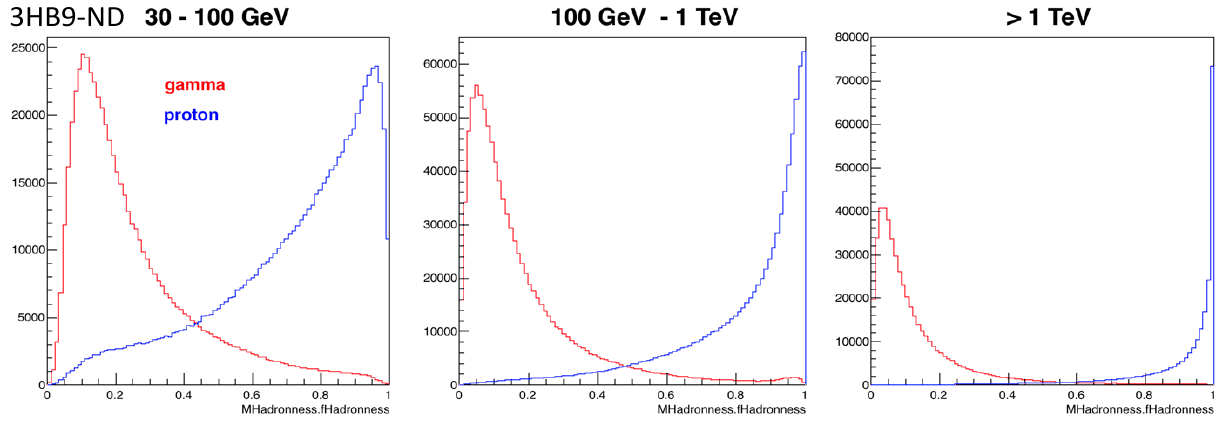
\includegraphics[width=.9\textwidth]{pics/hadroness_abelardo}
    \end{frame}



    \begin{frame}{Full List of Features for RandomForest}
        \begin{itemize}
         \item impact\_dist - distance between telescope and reconstructed impact position
         \item sum\_signal\_evt - total signal on all selected telescopes in the event
         \item sum\_signal\_cam - total signal on the current camera
         \item max\_signal\_cam - signal of the highest intensity pixel in the camera
         \item N\_LST - number of selected LSTs in the event
         \item N\_MST - number of selected MSTs in the event
         \item N\_SST - number of selected SSTs in the event
         \item Hillas width
         \item Hillas length
         \item Hillas skewness
         \item Hillas kurtosis
         \item h\_max - reconstructed height of shower maximum
         \item err\_est\_pos - error estimator of the reconstructed impact position
         \item err\_est\_dir - error estimator of the reconstructed shower direction
        \end{itemize}


    \end{frame}


    \begin{frame}{Event Weights}
        \begin{itemize}
            \item next step: reweighting of MC events to correspond to expected physical
                flux (e.g. Crab nebula for gammas, CR for protons)
            \only<-2>{
                \item simple binned approach:
                    \begin{itemize}
                        \item construct energy-binned selection efficiencies from MC
                        \item apply these on the energy-binned histogram of expected
                            \emph{arriving} events from the source
                        \item \textrightarrow\ get the number of expected selected events
                    \end{itemize}
                \only<2>{
                    \item \textbf{but:} it's binned... not optimal (but implemented anyway)
                }
            }
            \only<3>{
                \item instead: event-by-event weight that considers the generator
                    spectrum:
                \item $w(E) = A_\mathrm{gen} \times I_\Theta \times E^\gamma \times I_E
                    \times T_\mathrm{obs}/ N_\mathrm{gen}$\\ with:
                    \begin{itemize}
                        \item $A_\mathrm{gen}$: MC generator Area
                        \item $I_\Theta = 2 \pi (1-\cos\vartheta)$: angular phase space
                            factor for diffuse flux
                        \item $E^\gamma$: considers that MC events have been drawn with an
                            $E^{-2}$ spectrum
                        \item $\gamma$: spectral index of the MC generator (here equal 2)
                        \item $I_E =
                            (E_\mathrm{max}^{(1-\gamma)} - E_\mathrm{min}^{(1-\gamma)})
                            / (1-\gamma)$: energy phase space factor
                        \item $T_\mathrm{obs}$: assumed observation time
                        \item $N_\mathrm{gen}$: number of generated MC events
                    \end{itemize}
                \item $w(E) \times \varPhi(E)$ gives weight for every MC event so that
                    their energy distribution looks like the selected events from the
                    assumed flux $\varPhi$
            }
        \end{itemize}
    \end{frame}



    \begin{frame}{Effective Areas}{after reconstruction}
        \centering
        \setlength{\figureheight}{7cm}
        \setlength{\figurewidth}{.75\textwidth}
        % This file was created by matplotlib2tikz v0.6.13.
\begin{tikzpicture}

\definecolor{color0}{rgb}{1,0.647058823529412,0}

\begin{axis}[
xlabel={$E_\mathrm{MC} / \mathrm{TeV}$},
ylabel={$A_\mathrm{eff} / \mathrm{m}^2$},
xmin=0.00211134817886532, xmax=899.274928164032,
ymin=1.00562006408878, ymax=21315876.6110353,
xmode=log,
ymode=log,
width=\figurewidth,
height=\figureheight,
tick align=outside,
tick pos=left,
x grid style={lightgray!92.026143790849673!black},
y grid style={lightgray!92.026143790849673!black},
legend cell align={left},
legend entries={{gamma -- wavelets},{gamma -- tailcuts}},
legend style={at={(0.97,0.03)}, anchor=south east, draw=white!80.0!black}
]
\addlegendimage{mark=square*, mark size=1,thick, darkorange}
\addlegendimage{mark=square*, mark size=1,thick, darkred}

\addplot [thick, darkorange, mark=square*, mark size=1, mark options={solid}]
table {%
0.00380573560867088 104.292050900348
0.00585001340673278 968.967668287292
0.00899238948207052 7533.63446475569
0.013822715090565 34801.9278898888
0.0212476842618853 92235.0817647462
0.032661028136283 181879.261476612
0.0502051303930861 343712.448130601
0.0771731712568687 545266.876795822
0.118627286000679 716156.292113538
0.182348771661166 947681.239601108
0.280298704011029 1474390.96605585
0.430863135268352 2250212.75430304
0.662304315634544 3049679.78686871
1.01806576288997 3762784.43176057
1.56492698764273 4351856.953396
2.40553858691859 4785330.1640352
3.69769065192668 5134925.18085367
5.68393133733117 5645265.93032058
8.73709525448317 6068102.09381617
13.4302877630741 6449984.10416134
20.6444618200111 6891702.22033018
31.7337804934973 7313054.86553936
48.779805121068 7479859.13887663
74.9822224344482 8172117.46066107
115.259453522925 8110189.35283733
177.171884149169 8287237.96831868
272.3410147587 7817630.70205645
};

\addplot [semithick, darkred, mark=square*, mark size=1, mark options={solid}]
table {%
0.0102662682325922 3877.94577358886
0.0162709386338152 17386.0268360001
0.0257876998756863 43793.0872423286
0.0408707499822055 90939.0359219867
0.0647757734175777 169384.548024118
0.102662682325922 244004.783338918
0.162709386338152 324399.91194212
0.257876998756863 498794.096970875
0.408707499822055 797494.775322087
0.647757734175777 1124694.32525397
1.02662682325922 1415193.35227575
1.62709386338152 1656458.92888728
2.57876998756863 1824244.83133428
4.08707499822055 1981166.87228011
6.47757734175776 2176801.39484593
10.2662682325922 2345979.03855049
16.2709386338152 2498400.37734693
25.7876998756863 2724560.18764535
40.8707499822055 2728825.60094387
64.7757734175776 2977703.22987971
102.662682325922 3211631.88154772
162.709386338152 3010656.17896682
257.876998756863 3081750.81357757
};

\end{axis}

\node[anchor=west] at ({$(current bounding box.south west)!0.5!(current bounding box.south east)$}|-{$(current bounding box.south west)!0.5!(current bounding box.north west)$})
{factor 2 improvement throughout};

\end{tikzpicture}


    \end{frame}


    \begin{frame}{Quality cuts}
        \begin{itemize}
            \item energy-binned finding cuts to minimise sensitivity
            \item numerical fit simultaneous in gammaness and direction error
            \item $N_\gamma > 10$ and $N_\gamma > 0.05 * (N_\mathrm{p} + N_\mathrm{e})$
                taken into account
        \end{itemize}

        \centering
        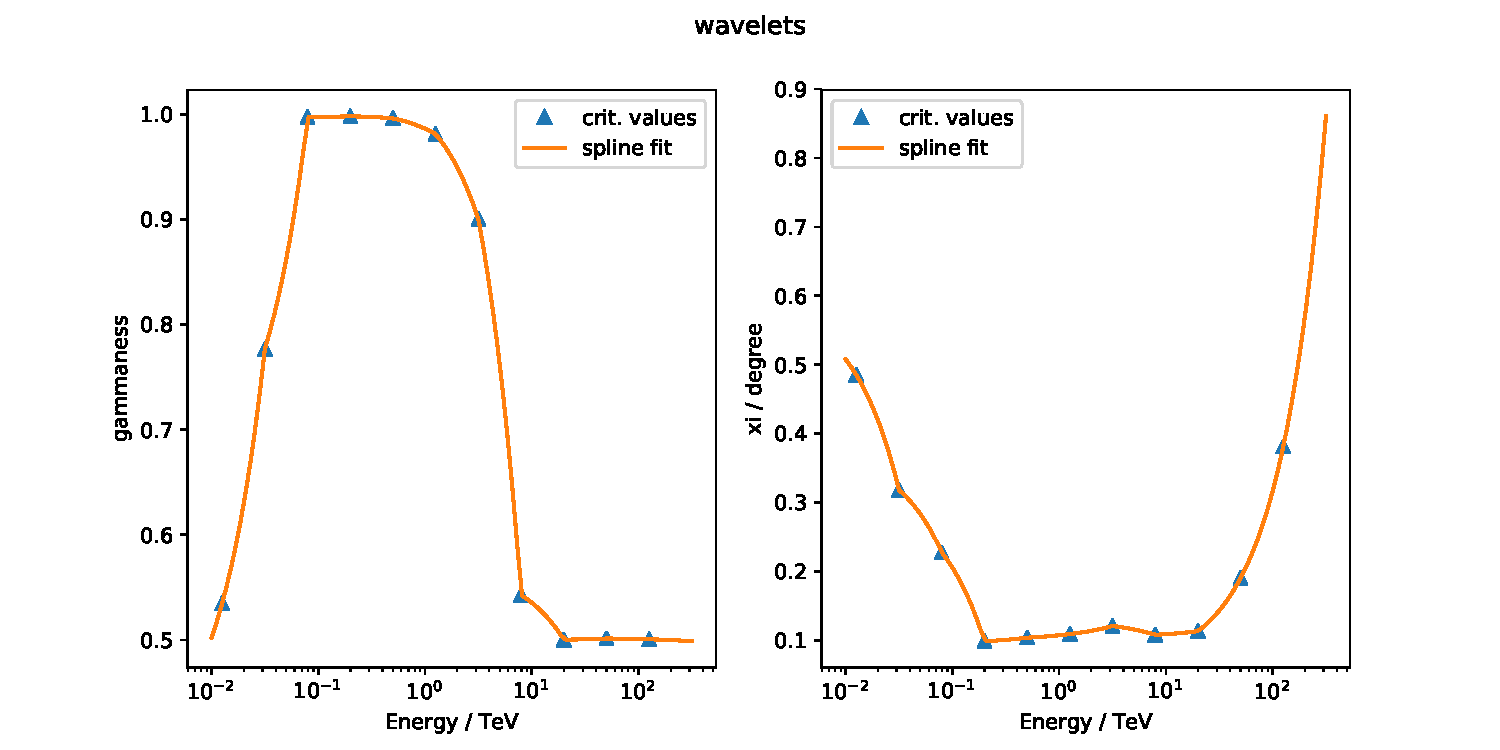
\includegraphics[width=.9\textwidth]{pics/cuts_vs_E_wave}

    \end{frame}


    \begin{frame}{Event Rates}
        {after gammaness only cut / after gammaness + theta cut}
        \begin{columns}
            \setlength{\figureheight}{7.cm}
            \setlength{\figurewidth}{.5\textwidth}
            \column{.5\textwidth}
                % This file was created by matplotlib2tikz v0.6.13.
\begin{tikzpicture}

\definecolor{color0}{rgb}{1,0.647058823529412,0}

\begin{axis}[
title={gammaness cut only},
xlabel={$E_\mathrm{MC} / \mathrm{TeV}$},
ylabel={event rate: $\frac{dN}{dt} / s^{-1}$},
xmin=0.00618603833675911, xmax=427.969290866181,
ymin=3.00082536021692e-06, ymax=1425.22673376302,
xmode=log,
ymode=log,
width=\figurewidth,
height=\figureheight,
tick align=outside,
tick pos=left,
x grid style={lightgray!92.026143790849673!black},
y grid style={lightgray!92.026143790849673!black},
legend entries={{proton},{electron},{gamma}},
legend style={draw=white!80.0!black},
legend cell align={left}
]
\addlegendimage{no markers, blue}
\addlegendimage{no markers, red}
\addlegendimage{no markers, color0}
\addplot [semithick, blue]
table {%
0.0102662682325922 14.4410286378731
0.0162709386338152 68.1282575451236
0.0257876998756863 196.831109029396
0.0408707499822055 381.107811985999
0.0647757734175777 558.349344639764
0.102662682325922 574.766020946227
0.162709386338152 451.272270027204
0.257876998756863 239.719833423547
0.408707499822055 91.1728989332365
0.647757734175777 32.478019110472
1.02662682325922 13.9404180310938
1.62709386338152 7.98637299957408
2.57876998756863 6.37082013995349
4.08707499822055 5.48476653234429
6.47757734175776 4.58428086227377
10.2662682325922 3.78894322952562
16.2709386338152 2.82245298483107
25.7876998756863 1.68021029985779
40.8707499822055 0.818784775201811
64.7757734175776 0.374289692376388
102.662682325922 0.177110514104366
162.709386338152 0.0711807057831022
257.876998756863 0.0275230802277724
};
\addplot [semithick, red]
table {%
0.0102662682325922 8.27614931004342
0.0162709386338152 26.6942079383687
0.0257876998756863 37.3601834692879
0.0408707499822055 29.0649089315294
0.0647757734175777 16.2463924124159
0.102662682325922 4.70927687423436
0.162709386338152 2.07643109266826
0.257876998756863 0.908731433767453
0.408707499822055 0.41542459727414
0.647757734175777 0.253953771371995
1.02662682325922 0.186103016063136
1.62709386338152 0.118976001229179
2.57876998756863 0.0699504728476827
4.08707499822055 0.0410830316033835
6.47757734175776 0.0218189543160713
10.2662682325922 0.0095795106548816
16.2709386338152 0.00373962538333403
25.7876998756863 0.0014154196076509
40.8707499822055 0.000449764357734886
64.7757734175776 0.000150302488377525
102.662682325922 4.68447176118692e-05
162.709386338152 1.65797955046097e-05
257.876998756863 7.44103925923506e-06
};
\addplot [semithick, color0]
table {%
0.0102662682325922 1.47065529732174
0.0162709386338152 3.17244809085737
0.0257876998756863 3.73511676736365
0.0408707499822055 3.19331481914353
0.0647757734175777 2.03403314863314
0.102662682325922 0.965907457845373
0.162709386338152 0.623365960660649
0.257876998756863 0.419562163216652
0.408707499822055 0.304287650769209
0.647757734175777 0.257492949079507
1.02662682325922 0.228921140089898
1.62709386338152 0.173760178806027
2.57876998756863 0.114703030316718
4.08707499822055 0.0719500485113641
6.47757734175776 0.0445750924504388
10.2662682325922 0.0254793141552946
16.2709386338152 0.0136660339342172
25.7876998756863 0.00737575156003909
40.8707499822055 0.00361992566379874
64.7757734175776 0.00187474439877034
102.662682325922 0.000965560508863483
162.709386338152 0.000424944090235254
257.876998756863 0.000197397564768067
};
\end{axis}

\end{tikzpicture}

            \column{.5\textwidth}
                % This file was created by matplotlib2tikz v0.6.13.
\begin{tikzpicture}

\definecolor{color0}{rgb}{1,0.647058823529412,0}

\begin{axis}[
title={gammaness + theta cuts},
xlabel={$E_\mathrm{MC} / \mathrm{TeV}$},
ylabel={event rate: $\frac{dN}{dt} / s^{-1}$},
xmin=0.00618603833675911, xmax=427.969290866181,
ymin=9.19555792162028e-08, ymax=51.2963274164015,
xmode=log,
ymode=log,
width=\figurewidth,
height=\figureheight,
tick align=outside,
tick pos=left,
x grid style={lightgray!92.026143790849673!black},
y grid style={lightgray!92.026143790849673!black},
legend entries={{proton},{electron},{gamma}},
legend style={draw=white!80.0!black},
legend cell align={left}
]
\addlegendimage{no markers, blue}
\addlegendimage{no markers, red}
\addlegendimage{no markers, color0}
\addplot [semithick, blue]
table {%
0.0102662682325922 0.534196036123186
0.0162709386338152 2.86857064396828
0.0257876998756863 9.09682062507665
0.0408707499822055 16.9207729764603
0.0647757734175777 20.5360880954089
0.102662682325922 18.4855559914912
0.162709386338152 12.4380026158078
0.257876998756863 6.05169043493176
0.408707499822055 2.57978661398846
0.647757734175777 1.03096007874168
1.02662682325922 0.402803002778079
1.62709386338152 0.148273706572368
2.57876998756863 0.0622181278618777
4.08707499822055 0.0285463493433057
6.47757734175776 0.0198566042476851
10.2662682325922 0.0158968961631879
16.2709386338152 0.00869974809889164
25.7876998756863 0.00458993298897727
40.8707499822055 0.00318512359268756
64.7757734175776 0.00202863329412002
102.662682325922 0.00209809411562358
162.709386338152 0.000666480611140529
257.876998756863 0.000637415649452143
};
\addplot [semithick, red]
table {%
0.0102662682325922 0.359717171454994
0.0162709386338152 1.01623618037542
0.0257876998756863 1.16892897307897
0.0408707499822055 0.655326174489666
0.0647757734175777 0.219066308093995
0.102662682325922 0.0528060507032044
0.162709386338152 0.0156659397952957
0.257876998756863 0.00417989868186608
0.408707499822055 0.0031105691543541
0.647757734175777 0.00140042110176421
1.02662682325922 0.00088797036839662
1.62709386338152 0.00027032587360332
2.57876998756863 6.40735164142421e-05
4.08707499822055 0.000127375128990712
6.47757734175776 1.95857261786134e-05
10.2662682325922 2.34824583393573e-05
16.2709386338152 1.38187905217314e-06
25.7876998756863 5.11588466664155e-07
40.8707499822055 5.65664026524044e-07
64.7757734175776 0
102.662682325922 7.6183674003308e-07
162.709386338152 0
257.876998756863 2.2969240671955e-07
};
\addplot [semithick, color0]
table {%
0.0102662682325922 0.700812063344183
0.0162709386338152 1.70048104680533
0.0257876998756863 2.08951356921284
0.0408707499822055 1.89646291028436
0.0647757734175777 1.38732213796251
0.102662682325922 0.759141678832288
0.162709386338152 0.471927073516024
0.257876998756863 0.293936004795124
0.408707499822055 0.237171253485485
0.647757734175777 0.199078224472734
1.02662682325922 0.169325823608296
1.62709386338152 0.134283206790291
2.57876998756863 0.096700005269656
4.08707499822055 0.0643161386708638
6.47757734175776 0.0403926994003394
10.2662682325922 0.0232275402411547
16.2709386338152 0.012443012239568
25.7876998756863 0.00677563369856345
40.8707499822055 0.00340674625794119
64.7757734175776 0.00179057338914653
102.662682325922 0.00093696184858628
162.709386338152 0.00041340838124096
257.876998756863 0.000192458367281749
};
\end{axis}

\end{tikzpicture}

        \end{columns}

    \end{frame}


    \begin{frame}{on-axis point-source Sensitivity}
        \setlength{\figureheight}{6.5cm}
        \setlength{\figurewidth}{.85\textwidth}
        \centering
        % This file was created by matplotlib2tikz v0.6.13.
\begin{tikzpicture}

\definecolor{color0}{rgb}{1,0.549019607843137,0}

\begin{axis}[
xlabel={$E_\mathrm{reco}$ / $\mathrm{TeV}$},
ylabel={$E^2 \Phi /$ $\mathrm{\frac{erg}{s\,cm^{2}}}$},
xmin=0.01, xmax=200,
ymin=5e-15, ymax=5e-10,
xmode=log,
ymode=log,
width=\figurewidth,
height=\figureheight,
xtick={0.001,0.01,0.1,1,10,100,1000,10000},
xticklabels={,${10^{-2}}$,${10^{-1}}$,${10^{0}}$,${10^{1}}$,${10^{2}}$,,},
ytick={1e-16,1e-15,1e-14,1e-13,1e-12,1e-11,1e-10,1e-09,1e-08},
yticklabels={,,${10^{-14}}$,${10^{-13}}$,${10^{-12}}$,${10^{-11}}$,${10^{-10}}$,,},
tick align=outside,
tick pos=left,
xmajorgrids,
x grid style={lightgray!92.026143790849673!black},
ymajorgrids,
y grid style={lightgray!92.026143790849673!black},
legend entries={{Crab Nebula},{Crab Nebula / 10},{Crab Nebula / 100},{reference},{wavelets},{tailcuts}},
legend style={opacity=.75,draw=white!80.0!black},
legend cell align={left}
]
\addlegendimage{no markers, red}
\addlegendimage{no markers, red}
\addlegendimage{no markers, red}
\addlegendimage{mark=square*, mark size=1, black}
\addlegendimage{thick,mark=square*, mark size=1.5, red!54.509803921568626!black}
\addlegendimage{thick,mark=square*, dashed, mark size=1.5, color0}
\addplot [semithick, red, dashed]
table {%
0.01 4.8065298624e-10
0.0191095297497044 3.47701564547967e-10
0.0365174127254838 2.51525282168409e-10
0.0697830584859866 1.81951920901322e-10
0.133352143216332 1.31622957478741e-10
0.254829674797935 9.52152791222591e-11
0.486967525165863 6.88781771203854e-11
0.930572040929699 4.98260712688296e-11
1.77827941003892 3.60438891079729e-11
3.39820832894256 2.60739389830356e-11
6.49381631576211 1.88617352598802e-11
12.4093776075172 1.36444691860818e-11
23.7137370566166 9.87032936285202e-12
45.3158363760082 7.14013864537556e-12
86.5964323360065 5.16513461719523e-12
165.481709994318 3.73642823182815e-12
316.227766016838 2.702910372389e-12
};
\addplot [semithick, red, opacity=0.66, dashed]
table {%
0.01 4.8065298624e-11
0.0191095297497044 3.47701564547967e-11
0.0365174127254838 2.51525282168409e-11
0.0697830584859866 1.81951920901322e-11
0.133352143216332 1.31622957478741e-11
0.254829674797935 9.52152791222591e-12
0.486967525165863 6.88781771203854e-12
0.930572040929699 4.98260712688296e-12
1.77827941003892 3.60438891079729e-12
3.39820832894256 2.60739389830356e-12
6.49381631576211 1.88617352598802e-12
12.4093776075172 1.36444691860818e-12
23.7137370566166 9.87032936285202e-13
45.3158363760082 7.14013864537556e-13
86.5964323360065 5.16513461719523e-13
165.481709994318 3.73642823182815e-13
316.227766016838 2.702910372389e-13
};
\addplot [semithick, red, opacity=0.33, dashed]
table {%
0.01 4.8065298624e-12
0.0191095297497044 3.47701564547967e-12
0.0365174127254838 2.51525282168409e-12
0.0697830584859866 1.81951920901322e-12
0.133352143216332 1.31622957478741e-12
0.254829674797935 9.52152791222591e-13
0.486967525165863 6.88781771203854e-13
0.930572040929699 4.98260712688296e-13
1.77827941003892 3.60438891079729e-13
3.39820832894256 2.60739389830356e-13
6.49381631576211 1.88617352598802e-13
12.4093776075172 1.36444691860818e-13
23.7137370566166 9.87032936285202e-14
45.3158363760082 7.14013864537556e-14
86.5964323360065 5.16513461719523e-14
165.481709994318 3.73642823182815e-14
316.227766016838 2.702910372389e-14
};
\addplot [black, mark=square*, mark size=1, mark options={solid}]
table {%
0.0158489319246111 6.87978e-11
0.0251188643150958 1.87765e-11
0.0398107170553497 7.00645e-12
0.0630957344480193 1.77677e-12
0.1 8.19263e-13
0.158489319246111 4.84879e-13
0.251188643150958 3.00256e-13
0.398107170553497 2.07787e-13
0.630957344480193 1.4176e-13
1 1.06069e-13
1.58489319246111 8.58209e-14
2.51188643150958 6.94294e-14
3.98107170553497 6.69301e-14
6.30957344480193 7.61169e-14
10 7.13895e-14
15.8489319246111 9.49376e-14
25.1188643150958 1.25208e-13
39.8107170553497 1.91209e-13
63.0957344480193 3.11611e-13
100 4.80354e-13
};
\addplot [thick, red!54.509803921568626!black, mark=square*, mark size=1.5, mark options={solid}]
table {%
0.01 8.97732586049047e-12
0.0158489319246111 1.31346379449665e-12
0.0251188643150958 3.5054272503888e-13
0.0398107170553497 2.20023527007935e-13
0.0630957344480193 1.19125140546455e-13
0.1 5.02638770771275e-14
0.158489319246111 3.68130354957728e-14
0.251188643150958 1.85789074858261e-14
0.398107170553497 1.78405006049022e-14
0.630957344480193 1.75830920476962e-14
0.999999999999999 1.50644459321183e-14
1.58489319246111 1.67622759929585e-14
2.51188643150958 1.63271747349374e-14
3.98107170553497 2.05783453205216e-14
6.30957344480193 2.80892276680632e-14
9.99999999999999 4.29435956270557e-14
15.8489319246111 4.83396995601958e-14
25.1188643150958 7.372821303281e-14
39.8107170553497 1.12993266358001e-13
63.0957344480193 1.34167205548644e-13
99.9999999999998 4.64349558715434e-13
158.489319246111 4.89513853606016e-13
251.188643150958 3.04006128074338e-12
};
\addplot [thick, color0, dashed, mark=square*, mark size=1.5, mark options={solid}]
table {%
0.01 1.0647312887569e-11
0.0158489319246111 5.48328573254468e-13
0.0251188643150958 2.03240768651982e-13
0.0398107170553497 1.85101950259334e-13
0.0630957344480193 1.45644685634984e-13
0.1 9.3584040552676e-14
0.158489319246111 6.39896948769896e-14
0.251188643150958 7.04173738077233e-14
0.398107170553497 4.35544586859766e-14
0.630957344480193 4.77959201023667e-14
0.999999999999999 4.44003948867611e-14
1.58489319246111 4.29734441683112e-14
2.51188643150958 4.96463296384831e-14
3.98107170553497 5.84962814364508e-14
6.30957344480193 7.60528735010101e-14
9.99999999999999 7.35841968805884e-14
15.8489319246111 9.12710099525779e-14
25.1188643150958 1.35556556243919e-13
39.8107170553497 1.86570122576284e-13
63.0957344480193 1.94358919798559e-13
99.9999999999998 6.49662441457101e-13
158.489319246111 4.67302879193594e-13
251.188643150958 4.61054256328862e-12
};
\path [draw=black, fill opacity=0] (axis cs:0,5e-15)
--(axis cs:0,5e-10);

\path [draw=black, fill opacity=0] (axis cs:1,5e-15)
--(axis cs:1,5e-10);

\path [draw=black, fill opacity=0] (axis cs:0.01,0)
--(axis cs:200,0);

\path [draw=black, fill opacity=0] (axis cs:0.01,1)
--(axis cs:200,1);

\node[rotate=30, scale=5,red, opacity=.5] at (axis cs: 1,1e-12) {PRELIMINARY};

\end{axis}


\end{tikzpicture}

        \setlength{\figureheight}{3.5cm}
        % This file was created by matplotlib2tikz v0.6.13.
\begin{tikzpicture}

\definecolor{color0}{rgb}{0.12156862745098,0.466666666666667,0.705882352941177}

\begin{axis}[
xlabel={E / $\mathrm{TeV}$},
ylabel={ratio},
xmin=0.0102329299228075, xmax=154.881661891248,
ymin=0.248832056335424, ymax=3.95881393788217,
xmode=log,
width=\figurewidth,
height=\figureheight,
tick align=outside,
tick pos=left,
x grid style={lightgray!92.026143790849673!black},
y grid style={lightgray!92.026143790849673!black},
legend cell align={left},
legend entries={{Sens$_\text{tail}$ / Sens$_\text{wave}$}},
legend style={at={(0.97,0.03)}, anchor=south east, draw=white!80.0!black}
]
\addlegendimage{no markers, color0}
\addplot [semithick, color0]
table {%
0.0158489319246111 0.417467596405731
0.0251188643150958 0.579788864907809
0.0398107170553497 0.841282533629501
0.0630957344480193 1.22261921343285
0.1 1.86185479502657
0.158489319246111 1.73823467734242
0.251188643150958 3.79017839781186
0.398107170553497 2.44132491854006
0.630957344480193 2.71828868169004
0.999999999999999 2.94736328749383
1.58489319246111 2.56369983326629
2.51188643150958 3.04071772639564
3.98107170553497 2.84261346212884
6.30957344480193 2.70754591047302
9.99999999999999 1.71350805180897
15.8489319246111 1.88811702974945
25.1188643150958 1.83859815215642
39.8107170553497 1.65116142394863
63.0957344480193 1.4486320930944
99.9999999999998 1.39908056175247
};
\end{axis}

\end{tikzpicture}


    \end{frame}



    \begin{frame}{Summary}
        \begin{itemize}
            \item ctapipe can produce sensitivity curves
            \item wavelets outperforms tailcuts
            \begin{itemize}
                \item angular resolution: 30 \% -- 80 \%
                \item effective area: 100 \%
                \item sensitivity: 100 \% -- 200 \%
            \end{itemize}
            \item gain over reference at low energies very large
            \item maybe still normalisation problem?
            \item will investigate further

        \end{itemize}

    \end{frame}

\end{document}





    \backup[hide]{
        \frame{
            not shown
        }
    }

\end{document}
